\chapter{A função \texorpdfstring{$\zeta$}{zeta} de Riemann}
\chaptermark{}

\hfill%
\begin{minipage}{10cm}
    \begin{flushright}
    \rightskip=0.5cm
        \textit{%
            ``If I were to awaken after having slept for a thousand years, my first question would be: Has the Riemann hypothesis been proven?''
        }
        \\[0.1cm]
    \rightskip=0.5cm
    --- David Hilbert
    \end{flushright}
\end{minipage}

\section{Funções Inteiras}
    \subsection{Fórmula de Jensen e número de zeros}
    
    Nesta seção, mostraremos o Teorema da Fórmula de Jensen, que relaciona os zeros 
    de uma função em um disco com a média logarítmica do módulo desta função ao 
    longo do bordo do disco. Não é claro, a princípio, o significado desta fórmula,
    mas ela permitirá que cheguemos a várias conclusões muito interessantes. 
    Vamos poder, por exemplo, estabelecer estimativas a respeito da quantidade 
    de zeros de uma função no interior de um disco de raio dado.
    
    Inicialmente, começamos mostrando dois resultados que nos serão bastante úteis.
    Primeiro, observe que, se $f$ é holomorfa num disco de raio $R$ e centro $z_0$,
    pela fórmula integral de Cauchy, com $\gamma = z_0 + re^{i\theta}$ e $0 < r < R$,
    temos
    %
    \begin{align*}
        f(z_0) &= \frac{1}{2\pi i}\int_\gamma \frac{f(w)}{w - z_0} \, dw \\
        &= \frac{1}{2\pi i} \int_{0}^{2\pi} \frac{f(z_0 + re^{i\theta})}{z_0 + re^{i\theta} - z_0} rie^{i\theta} \, d\theta \\
        &= \frac{1}{2\pi}\int_{0}^{2\pi}f(z_0 + re^{i\theta}) \, d\theta.
    \end{align*}
    %
    Portanto,
    %
    \begin{equation}
    \label{eq-representacao-int-re-f(z)}
        \Re(f(z_0)) 
        = \frac{1}{2\pi}\int_{0}^{2\pi}\Re(f(z_0 + re^{i\theta})) \, d\theta.
    \end{equation}
    %
    Anteriormente, tentamos definir um ramo para o logaritmo de uma função $f(z)$, 
    mas o princípio do argumento nos foi um obstáculo porque $f$ tinha um zero 
    no interior da região delimitada por $\y$. Tanto zeros quanto singularidades 
    podem trazer problemas  se quisermos fazer uma construção daquele tipo, justamente
    por conta do princípio do argumento. 
    
    Se $G$ é uma conjunto aberto simplesmente conexo contendo 1 e que não contém 0,
    podemos definir um ramo do logaritmo $F(z) = \log_G(z)$ tal que $F$ é holomorfa 
    em $G$ e coincide com o logaritmos de base $e$ num intervalo real contendo 1. 
    Além disso, $\exp(F(z)) = z$ para todo $z \in G$. Lembre-se que podemos definir
    %
    \begin{equation*}
        \ln{x} = \int_{0}^{x}\frac{1}{t} \, dt.
    \end{equation*}    
    %
    Tomando esta situação como inspiração, definimos
    %
    \begin{equation*}
        F(z) = \int_\y \frac{1}{z} \, dz,
    \end{equation*}
    %
    onde $\y$ é uma curva contida em $G$ conectando 1 a $z$. Observe que $F$ está 
    bem definida, pois $G$ é um conjunto simplesmente conexo, ou seja qualquer 
    curva fechada é homotópica a zero, como no Teorema de Monodromia 
    (Teorema \ref{teo-monodromia}). Mais precisamente, se $\beta$ e $\y$ são 
    duas curvas contidas em $G$ conectando 1 a $z$, temos
    %
    \begin{equation*}
        \int_{\y * \beta^-} \frac{1}{z} \, dz = 0,
    \end{equation*}    
    %
    pois $1/z$ é holomorfa na região interior à concatenação dessas curvas. 
    A hipótese de $G$ ser simplesmente conexo é importante, pois, 
    num certo sentido, estamos fazendo continuações analíticas 
    no sentido do Teorema de Monodromia.
    
    Observe que 
    %
    \begin{equation*}
        \frac{d}{dz}F(z) = \frac{1}{z},
    \end{equation*}    
    %
    então 
    \begin{align*}
        \frac{d}{dz}(z\exp{-F(z)}) &= \exp{(-F(z))} + z\exp{(-F(z))}\frac{-1}{z} \\
        & = 0.
    \end{align*}
    %
    Como $G$ é conexo, concluímos que $z\exp{-F(z)}$ é constante. Calculando o 
    valor da expressão em $z = 1$, obtemos o resultado. Mostramos agora a última
    parte. Como $1 \in G$ e $G$ é aberto, existe um intervalo aberto 
    $I \subseteq \R$ contendo $1$ tal que, para $x \in I$,
    %
    \begin{equation*}
        F(x) = \int_{1}^{x} \frac{1}{t} \, dt = \ln{x}.
    \end{equation*}    
    %
    O próximo lema é, essencialmente, uma repetição dos argumentos acima, mas 
    num contexto mais geral.
    %
    \begin{lema}%Teorema 6.2 cap 3 Stein
    \label{lema-ramo-log}
        Se $f : G \to \C$ é holomorfa e não se anula na região simplesmente conexa 
        $G \subseteq C$, então existe uma função $g$ definida e holomorfa em $G$ 
        tal que 
        %
        \begin{equation*}
            f(z) = \exp{g(z)}
        \end{equation*}
        %
        para todo $z \in G$.
    \end{lema}
    %
    \begin{proof}
        Em termos práticos, $g(z) = \log f(z)$ se pudermos dar sentido a essa
        expressão. Seja $z_0 \in G$. Seguindo as ideias que mostramos anteriormente,
        definimos
        %
        \begin{equation*}
            g(z) = \int_{\y} \frac{f'(z)}{f(z)} \, dz, + C_0
        \end{equation*}
        %
        onde $\y$ é uma curva conectando $z_0$ a $z$ contida em $G$. Como $G$ é
        simplesmente conexo, $g$ está bem definida (i.e., independe da escolha de
        $\y$). A constante $C_0$ é escolhida de modo que $\exp(C_0) = f(z_0)$. 
        Além disso, observe que 
        %
        \begin{equation*}
            g'(z) = \frac{f'(z)}{f(z)}.
        \end{equation*}
        %
        Derivando a expressão $f(z)\exp{-g(z)}$ e usando a conexidade de $G$, vemos
        que ela é constante. O seu valor em $z = z_0$ é 1, então concluímos que 
        $f(z) = \exp{g(z)}$.
    \end{proof}
    %
    
    \medskip 
    
    
    A seguir, enunciamos e provamos o teorema que é o foco desta seção. O lema
    anterior e a observação no início da seção são usados fortemente para resolver
    integrais que seriam complicadas se tentássemos resolver explicitamente. 
    Denotamos por $D_R$ um disco centrado na origem com raio $R$.
    %
    \begin{teorema}[Fórmula de Jensen]
    \label{teo:form-jensen}
    \index{Fórmula!de Jensen}
    \index{Teorema!de Jensen}
        Sejam $G$ um aberto que contém o fecho do disco $D_R$ e $f$ uma função
        holomorfa em $G$ tal que $f(0) \neq 0$ e $f(z) \neq 0$ para 
        $z \in \partial D_R$. Denote por $z_1, \dots, z_N$ os zeros de $f$ no 
        interior de $D_R$ (listados com multiplicidade). 
        Então
        %
        \begin{equation}
        \label{eq-formula-jensen}
            \ln{|f(0)|} = \sum_{k = 1}^{N}\ln{\frac{|z_k|}{R}} 
            + \frac{1}{2\pi}\int_{0}^{2\pi}\ln{|f(Re^{i\theta})|} \, d\theta.
        \end{equation}
        %
    \end{teorema}
    %
    \begin{proof}
        Pelas propriedades do logaritmo e pela linearidade da integral, vemos que, 
        se duas funções satisfazem as hipóteses desse teorema, então o produto delas
        também satisfaz. Como os $z_j$ são os únicos zeros de $f$ no interior de
        $D_R$, a função $g:G -\{z_1, \dots, z_N\}\to \mathbb{C}$ dada por
        %
        \begin{equation*}
            g(z) = \frac{f(z)}{(z-z_1) \cdots (z-z_N)}
        \end{equation*}
        %
        tem apenas singularidades removíveis em $\overline{D}_R$. 
        Portanto podemos aplicar o Teorema de Riemann para
        garantir que $g$ admite uma extensão holomorfa, a todo $G$.  
        Além do mais, $g$ não se nula em $\overline{D}_R$. 
        Portanto temos
        %
        \begin{equation*}
            f(z) = (z-z_1)\cdots(z-z_N)g(z).
        \end{equation*}
        %
        Observe que se mostramos a validade da identidade
        \eqref{eq-formula-jensen} para funções do tipo $g(z)$ 
        (holomorfas e não se anulam em $\overline{D}_R$) e para as funções $z-z_j$ 
        o teorema fica demonstrado para $f$, pois ela é um produto destas funções.
        
        Como $G$ é aberto e contém $\overline{D}_R$, podemos encontrar $\Tilde{R}>R$
        tal que $D_{\Tilde{R}}$ está contido em $G$. Podemos, então, aplicar o 
        Lema \ref{lema-ramo-log} para a função $g$ e deduzir que existe uma função
        $h$ holomorfa em $D_{\Tilde{R}}$ tal que $g(z) = \exp(h(z))$. Segue que
        %
        \begin{equation*}
            |g(z)| = |\exp(h(z))| = e^{\Re{(h(z))}} 
            \implies \ln{|g(z)|} = \Re{(h(z))}.
        \end{equation*}
        %
        Usando última identidade acima e \eqref{eq-representacao-int-re-f(z)}
        a $\Re{(h(0))}$, obtemos 
        %
        \begin{align*}
            \ln{|g(0)|} = \Re(h(0)) &= \frac{1}{2\pi} 
            \int_{0}^{2\pi}\Re{(h(Re^{i\theta}))} \, d\theta \\
            &= \frac{1}{2\pi}\int_{0}^{2\pi}\ln{|g(Re^{i\theta})|} \, d\theta.
        \end{align*}
        %
        Mostrando a validade da Fórmula de Jensen para
        funções que não se anulam em $\overline{D}_R$.
        
        
        Resta mostrar que o resultado vale para uma função da forma $f(z) = z - w$,
        onde $w \in D_R$. Nosso objetivo é mostrar que vale
        %
        \begin{equation*}
            \ln{|w|} = \ln{\frac{|w|}{R}} 
            + \frac{1}{2\pi}\int_{0}^{2\pi}\ln{|Re^{i\theta} - w|} \, d\theta.
        \end{equation*}
        %
        Desenvolvendo os termos dessa soma onde é possível e notando que
        $|Re^{i\theta} - w| = R|e^{i\theta} - w/R|$, temos que o problema se 
        reduz a mostrar que vale
        %
        \begin{equation*}
            \int_{0}^{2\pi}\ln{|e^{i\theta} - a|} \, d\theta = 0,
        \end{equation*}
        %
        onde $|w/R| = |a| < 1$. Observe ainda que 
        $|e^{i\theta} - a| = |e^{i\theta}||1-ae^{i\theta}| = |1-ae^{i\theta}|$, 
        então reescrevemos a integral de interesse como
        %
        \begin{equation*}
            \int_{0}^{2\pi}\ln{|1 - ae^{i\theta}|} \, d\theta = 0.
        \end{equation*}
        %
        Explicitamente, esta integral se escreve como
        %
        \begin{equation*}
            \int_{0}^{2\pi}\ln{\sqrt{1 + |a|^2 - 2|a|\cos{\theta}}} \, d\theta,
        \end{equation*}
        %
        que não é tão simples de ser resolvida. A aplicação do 
        Lema \ref{lema-ramo-log} simplificará consideravelmente este cálculo. 
        
        Considere a função $F(z) = 1 - az$. $F$ não se anula e é holomorfa no 
        disco de raio $1$ centrado na origem, pois $|a| < 1$. Portanto, ela é
        holomorfa e não se anula num disco $D$ de raio $1 + \e$ centrado na origem,
        para algum $\e > 0$ suficientemente pequeno. 
        Este disco é uma região simplesmente
        conexa, então, pelo Lema \ref{lema-ramo-log}, existe uma função $G$ holomorfa
        em $D$ tal que 
        %
        \begin{equation*}
            F(z) = \exp(G(z)) \ \ \forall z \in D.
        \end{equation*}
        %
        
        Observe que $F(0) = 1$. Usando novamente a identidade
        \eqref{eq-representacao-int-re-f(z)} , temos
        %
        \begin{align*}
             0 = \ln{|F(0)|} &= \Re{(G(0))}\\
                &= \frac{1}{2\pi} \int_{0}^{2\pi}\Re{(G(e^{i\theta}))} \, d\theta \\
                &= \frac{1}{2\pi} \int_{0}^{2\pi}\ln{|F(e^{i\theta})|} \, d\theta \\
                &= \frac{1}{2\pi} \int_{0}^{2\pi}\ln{|1 - ae^{i\theta}|} \, d\theta .
        \end{align*}
        %
        O que encerra a prova do Teorema.
    \end{proof}
    
    
    
    
    \bigskip 
    
    
    
    Podemos ainda dar uma demonstração alternativa deste teorema que deixa mais explicita as ideias de extensão analítica contidas nesta demonstração. Observe que a fórmula de Jensen pode ser escrita na forma alternativa
    %
    \begin{equation*}
        \ln{\Big |f(0) \frac{R}{z_1}\cdots\frac{R}{z_N}\Big |} 
        = \frac{1}{2\pi}\int_{0}^{2\pi}\ln{|f(Re^{i\theta})|} \, d\theta, 
    \end{equation*}
    %
    onde usamos apenas as propriedades do logaritmo para reescrevê-la.
    
    Para uma função do tipo $g(z)$ acima, o teorema vale. Seja $f$ uma função
    satisfazendo as hipóteses do Teorema e considere a função
    %
    \begin{equation}\label{eq-aux-F-formula-jensen}
        F(z) = f(z)\frac{R^2 - z\overline{z}_1}{R(z-z_1)}\cdots
        \frac{R^2 - z\overline{z}_N}{R(z-z_N)}
    \end{equation}
    %
    definida em todo o $G$ exceto nos zeros de $f$. 
    Usando o Teorema de Riemann podemos garantir que $F$ admite uma extensão
    holomorfa a todo domínio $G$, 
    já que suas singularidades são todas removíveis. 
    Portanto, a menos de extensão, podemos assumir 
    que $F$ é uma função holomorfa em $G$. 
    Além disso, se $|z| = R$, então 
    %
    \begin{align*}
        \Big | \frac{R^2 - z\overline{z}_1}{R(z-z_j)} \Big | &= \Big | 
        \frac{R^2 - z\overline{z}_j}{R(z-z_j) \frac{R}{\overline{z}}} \Big | \\
        &= \Big | \frac{R^2 - z\overline{z}_j}{R^2-z_j\overline{z}}  \Big | \\
        &= 1.
    \end{align*}
    %
    Isto mostra que $|F(z)| = |f(z)|$ para todo $z \in \partial D_R$.
    Por hipótese, $f$ não anula $\partial D_R$. Consequentemente $F$ 
    não se anula no bordo de $D_R$. 
    Logo vale a fórmula de Jensen para $F$ e portanto
    %
    \begin{equation*}
        \ln{|F(0)|} = \frac{1}{2\pi}\int_{0}^{2\pi}\ln{|F(Re^{i\theta})|}\, d\theta.
    \end{equation*}
    %
    Usando a expressão de $F$ dada em 
    \eqref{eq-aux-F-formula-jensen}, 
    obtemos o resultado desejado.
    
    
    
    \bigskip 
    
    
    Agora, vamos usar a fórmula de Jensen para encontrar uma relação entre a
    taxa de crescimento de uma função inteira no infinito e o comportamento
    assintótico do número de zeros (contados com multiplicidade) desta
    função dentro dos discos $D(0,R)$ quando $R\to +\infty$.
    
    % Primeiro, note que podemos reescrever a fórmula de Jensen da seguinte forma:
    % %
    % \begin{align*}
    %     \ln|f(0)| = \sum_{j=1}^n \ln\left|\frac{z_j}{R}\right| 
    %     + \frac{1}{2\pi}\int_0^{2\pi} \ln|f(Re^{i\theta})| \, d\theta,
    % \end{align*}
    % %
    % usando as propriedades do logaritmo e do valor absoluto.
    
    Seja $f:U\subset\C\to\C$ é uma função holomorfa em $\overline{D(0,R)}$.
    Para cada $r\in (0,R)$ denotamos por $n_f(r) \equiv n(r)$ o número de zeros 
    de $f$, contados com multiplicidade, dentro do disco aberto $D(0,r)$.
    Note que segue diretamente da definição que se $0 < r_1 \leq r_2 < R$, então
    $n_f(r_1) \leq n_f(r_2)$, ou seja, $n_f$ é uma função não-decrescente. Usaremos
    esse fato no seguinte lema que, por sua vez, será o primeiro de dois resultados
    que nos permitirão extrair a relação entre: zeros e a ordem de uma função.
    
    % Vamos denotar por $n_f(r)$ o número zeros da função $f$ 
    % (contados com multiplicidade) no interior de um disco de raio $r$ e 
    % centro na origem. 
    % É fácil ver que $n_f$ é uma função não decrescente de $r$.
    %
    \begin{corolario}
    \label{corol:num-zeros}
        Se $z_1, \dots, z_N$ são os zeros de $f$ no interior de $D_R$, então
        %
        \begin{equation*}
            \int_{0}^{R}n_f(r) \, \frac{dr}{r} 
            = \sum_{k=1}^{N} \ln{\left |\frac{R}{z_k}\right|}.
        \end{equation*}
        %
    \end{corolario}
    %
    \begin{proof}
    Observe inicialmente que 
    %
    \begin{equation*}
        \ln{\left |\frac{R}{z_k}\right|} = \ln{R} - \ln{|z_k|} 
        = \int_{|z_K|}^{R} \, \frac{dr}{r}.
    \end{equation*}
    %
    Portanto, 
    %
    \begin{equation*}
        \sum_{k=1}^{N}\ln{\left |\frac{R}{z_k}\right|} 
        = \sum_{k=1}^{N}\int_{|z_k|}^{R} \, \frac{dr}{r}.
    \end{equation*}
    %
    Defina, para $k \in \{1, \dots, N\}$, as funções
    
    \begin{tabular}{%
    		@{}
    		m{.5\textwidth}
    		@{}
    		m{.5\textwidth}
    		@{}
    	}
    	\centering
    	$\dis
    	\eta_k(r) = 
        \begin{cases}
            1, &\text{se } r > |z_k| \\
            0, &\text{se } r \leq |z_k|
        \end{cases}
    	$
    	&
    	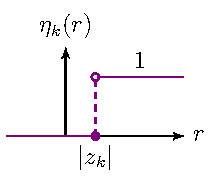
\includegraphics{Figuras/função salto.pdf} 
    \end{tabular}
    
    Então $n_f(r) = \dis{\sum_{k=1}^{N} \eta_k(r)}$. Segue que
    %
    \begin{align*}
        \sum_{k=1}^{N}\int_{|z_K|}^{R} \, \frac{dr}{r} 
        &= \sum_{k=1}^{N}\int_{|z_K|}^{R}\eta_k(r) \, \frac{dr}{r} \\
        &= \int_{|z_K|}^{R}\left(\sum_{k=1}^{N}\eta_k(r)\right) \, \frac{dr}{r} \\
        &= \int_{0}^{R}n_f(r) \, \frac{dr}{r}.
    \end{align*}
    %
    \end{proof}
    %
%\subsection{Ordem de crescimento e o número de zeros de uma função}
    % Agora, vamos usar a fórmula de Jensen para encontrar uma relação entre a
    % taxa de crescimento de uma função inteira no infinito e o comportamento
    % assintótico do número de zeros (contados com multiplicidade) desta
    % função dentro dos discos $D(0,R)$ quando $R\to +\infty$.
    
    % Primeiro, note que podemos reescrever a fórmula de Jensen da seguinte forma:
    % %
    % \begin{align*}
    %     \ln|f(0)| = \sum_{j=1}^n \ln\left|\frac{z_j}{R}\right| 
    %     + \frac{1}{2\pi}\int_0^{2\pi} \ln|f(Re^{i\theta})| \, d\theta,
    % \end{align*}
    % %
    % usando as propriedades do logaritmo e do valor absoluto.
    
    % Seja $f:U\subset\C\to\C$ é uma função holomorfa em $\overline{D(0,R)}$.
    % Para cada $r\in (0,R)$ denotamos por $n_f(r) \equiv n(r)$ o número de zeros 
    % de $f$, contados com multiplicidade, dentro do disco aberto $D(0,r)$.
    % Note que segue diretamente da definição que se $0 < r_1 \leq r_2 < R$, então
    % $n_f(r_1) \leq n_f(r_2)$, ou seja, $n_f$ é uma função não-decrescente. Usaremos
    % esse fato no seguinte lema que, por sua vez, será o primeiro de dois resultados
    % que nos permitirão extrair a relação entre zeros e a ordem de uma função.
    %
    % \begin{lema}
    % \label{lema:int-num-zeros}
    %     Sejam $R > 0$, $U\subseteq\C$ tal que $\overline{D(0,R)} \subseteq U$
    %     e $f:U\to\C$ uma função holomorfa. Se $z_1, z_2, \dots, z_n$ são zeros
    %     de $f$ em $D(0,R)$, então
    %     %
    %     \begin{equation*}
    %         \int_0^R n_f(r) \, \frac{dr}{r} 
    %         = \sum_{j=1}^n \ln\left|\frac{R}{z_j}\right|.
    %     \end{equation*}
    %     %
    % \end{lema}
    % %
    % \begin{proof}
    %     Note, primeiramente, que
    %     %
    %     \begin{equation*}
    %         \sum_{j=1}^n \ln\left|\frac{R}{z_j}\right| 
    %         = \sum_{j=1}^n \int_{|z_j|}^R \frac{1}{r} \, dr.
    %     \end{equation*}
    %     %
    %     Ademais, para cada $j=1, 2, \dots, n$, considere a função $\eta_j:\R\to\R$
    %     definida anteriormente:
    %     %
    %     \begin{equation*}
    %         \eta_j(r) 
    %         = \begin{cases}
    %         1, & |z_j| < r \\
    %         0, & |z_j| \geq r
    %         \end{cases}.
    %     \end{equation*}
    %     Daí, para cada $r$ fixado, temos
    %     %
    %     \begin{equation*}
    %         \sum_{j=1}^n \eta_j(r) = n_f(r),
    %     \end{equation*}
    %     %
    %     donde segue que
    %     %
    %     \begin{align*}
    %         \sum_{j=1}^n \int_{|z_j|}^R 1 \, \frac{dr}{r}
    %         = \sum_{j=1}^n \int_{0}^R \eta_j(r) \, \frac{dr}{r}
    %         = \int_{0}^R \left( \sum_{j=1}^n \eta_j(r) \right) \, \frac{dr}{r}
    %         = \int_{0}^R n_f(r) \, \frac{dr}{r},
    %     \end{align*}
    %     %
    %     como desejado.
    % \end{proof}
    %
    \noindent
    O segundo resultado que precisaremos é consequência imediata do 
    Corolário \ref{corol:num-zeros}.
    %
    \begin{corolario}
    \label{corol:jensen-com-zeros}
        Sejam $f:\C\to\C$ uma função inteira e $R>0$. Suponha que $f(0)\neq 0$
        e que $f(z)\neq 0$ para todo $z\in\partial D(0,R)$. Então
        %
        \begin{equation*}
            \int_0^R n_f(r) \, \frac{dr}{r}
            = \frac{1}{2\pi} \int_0^{2\pi} \ln|f(Re^{i\theta})| \, d\theta
            - \ln|f(0)|.
        \end{equation*}
        %
    \end{corolario}
    %
    \begin{proof}
       Pelo Corolário \ref{corol:num-zeros}, temos
       %
       \begin{equation*}
           \int_0^R n_f(r) \, \frac{dr}{r} 
           = \sum_{j=1}^n \ln\left|\frac{R}{z_j}\right|.
       \end{equation*}
       %
       Daí, basta usar esta identidade na fórmula de Jensen para obter o resultado.
    \end{proof}
    %
    \subsection{Funções de Ordem Finita de Crescimento}
    %
    \begin{definicao}[Ordem de Crescimento]
    \label{def:ordem-func}
    \index{Ordem de Crescimento}
        Seja $f:\C\to\C$ uma função inteira. Se existem um número positivo $\rho$
        e constantes $A,B>0$ tais que
        %
        \begin{equation*}
            |f(z)| \leq A\exp(B|z|^{\rho}),\quad  \forall z\in\C,
        \end{equation*}
        %
        dizemos que $f$ tem ordem de crescimento no máximo $\rho$. Definimos a
        ordem de crescimento de $f$ como sendo o número
        %
        \begin{equation*}
            \rho_f 
            \equiv 
            \inf 
            \left\{ 
                \rho > 0 :
                \begin{array}{c}
                    \exists m\ \textrm{constantes}\  
                    A\equiv A(\rho)>0\ \text{e}\ B\equiv B(\rho)>0\ \text{tais que}
                    \\[0.2cm]
                    |f(z)| \leq A\exp(B|z|^{\rho}), \quad \forall z\in\C
                \end{array}
            \right\}.
        \end{equation*}
        %
    \end{definicao}
    %
    Alguns exemplos são:
    %
    \begin{itemize}
        \item a função $f:\C\to\C$ dada por $f(z) = e^z$ tem ordem de crescimento 1;
        \item a função $g:\C\to\C$ dada por $g(z) = e^{\alpha z^2 + z}, \alpha\in\C^*$
        tem ordem de crescimento 2;
        \item a função $f:\C\to\C$ dada por $f(z) = e^{e^z}$ não tem ordem de
        crescimento finita.
    \end{itemize}
    %
    \begin{teorema}
    \label{teo:est-num-zeros}
        Se $f:\C\to\C$ tem ordem de crescimento no máximo $\rho$, então:
        %
        \begin{enumerate}[(i)]
            \item $n_f(r) \leq Cr^{\rho}$ para algum $C>0$ e $r\gg 1$;
            \item se $z_1, z_2, \dots$ denotam os zeros de $f$, com $z_k\neq 0$,
            então para todo $s>\rho$ temos
            %
            \begin{equation*}
                \sum_{k=1}^{\infty} \frac{1}{|z_k|^s} < + \infty.
            \end{equation*}
            %
        \end{enumerate}
        %
    \end{teorema}
    %
    \begin{proof}
       Primeiro vamos mostrar que a conclusão do item {\it (i)} é válida. 
       Observe que basta mostrar que vale a estimativa
       %
       \begin{equation*}
           n_f(r) \leq Cr^{\rho}
       \end{equation*}
       %
       no caso em que $f$ não se anula na origem. 
       De fato, se $f(0) = 0$ e $k$
       é a multiplicidade de $0$, então a função $F:\C^*\to\C$ dada por 
       $F(z) = f(z)/z^k$ admite uma extensão inteira que não se anula na origem
       e além do mais $n_F(r) = n_f(r) - k$. Logo, para todo $r\geqslant 1$ temos
       %
       \begin{align*}
           n_f(r) = n_F(r) + k &\leq Cr^{\rho} + k \\
                               &\leq Cr^{\rho} + kr^{\rho} \\
                               &= (C+k) r^{\rho}.
       \end{align*}
       %

       
       Já que estamos assumindo que $f(0) \neq 0$, podemos aplicar o 
       Corolário \ref{corol:jensen-com-zeros}, que diz que
       %
       \begin{equation*}
           \int_0^R n_f(x) \, \frac{dx}{x} 
           = \frac{1}{2\pi} \int_0^{2\pi} \ln|f(Re^{i\theta})| \, d\theta - \ln|f(0)|.
       \end{equation*}
       %
       Escolhendo $R = 2r$ temos, pelas propriedades da integral, que
       %
       \begin{align*}
           \int_r^{2r} n_f(x) \, \frac{dx}{x}
           \leq \int_0^{2r} n_f(x) \, \frac{dx}{x}
           = \frac{1}{2\pi} \int_0^{2\pi} \ln|f(2re^{i\theta})| \, d\theta - \ln|f(0)|.
       \end{align*}
       %
       Lembrando que $n_f$ é monótona não-decrescente, temos a seguinte estimativa:
       %
       \begin{align*}
           \int_r^{2r} n_f(x) \, \frac{dx}{x}
           \geq n_f(r) \int_r^{2r} \frac{dx}{x} 
           = n_f(r)[\ln(2r) - \ln(r)]
           = n_f(r)\ln(2).
       \end{align*}
       %
       Por outro lado, segue da hipótese de $f$ 
       ter ordem de crescimento no máximo $\rho$ que
       %
       \begin{align*}
           \left| \frac{1}{2\pi} \int_0^{2\pi} \ln|f(2re^{i\theta})| \, d\theta \right|
           &\leq \frac{1}{2\pi} \int_0^{2\pi} \big|\ln|f(2re^{i\theta})| \big| \, d\theta 
           \\[0.2cm]
           &\leq \frac{1}{2\pi} \int_0^{2\pi} \ln\left(Ae^{B(2r)^{\rho}}\right) 
           \, d\theta 
           \\[0.2cm]
           &= \ln A + B2^{\rho}r^{\rho} 
           \\[0.2cm]
           &\leq r^{\rho}\ln A + B2^{\rho}r^{\rho} 
           \\[0.2cm]
           &= (\ln A + 2^{\rho}B)r^{\rho}.
       \end{align*}
       %
       Usando essas duas estimativas e tomando $r\gg 1$ (suficientemente grande),
       temos
       %
       \begin{align*}
           n_f(r)\ln(2) \leq \int_r^{2r} n_f(x) \, \frac{dx}{x} 
                        &\leq \int_0^{2r} n_f(x) \, \frac{dx}{x} 
                        \\[0.2cm]
                        &= \frac{1}{2\pi}\int_0^{2\pi} \ln|f(2re^{i\theta})| \, d\theta
                        - \ln|f(0)| 
                        \\[0.2cm]
                        &\leq (\ln A + 2^{\rho}B)r^{\rho} + \big|\ln|f(0)|\big| 
                        \\[0.2cm]
                        &\leq (\ln A + 2^{\rho}B)r^{\rho} + \big|\ln|f(0)|\big|r^{\rho} 
                        \\[0.2cm]
                        &= [\ln A + 2^{\rho}B + \big|\ln|f(0)|\big|]r^{\rho},
       \end{align*}
       %
       donde segue que
       %
       \begin{equation*}
           n_f(r) \leq \frac{\ln A + 2^{\rho}B + \big|\ln|f(0)|\big|}{\ln(2)}r^{\rho} 
           \equiv Cr^{\rho}.
       \end{equation*}
       %
       
       \medskip 
       Para provar a validade da conclusão do item {\it (ii)}, basta notar que
       %
       \begin{align*}
           \sum_{\substack{k\in\N \\ |z_k|\geq 1}} \frac{1}{|z_k|^s}
           &= \sum_{j=0}^{\infty} 
           \sum_{\substack{k\in\N \\ 2^j \leq |z_k| < 2^{j+1}}} \frac{1}{|z_k|^s} 
           \\[0.3cm]
           &\leq \sum_{j=0}^{\infty} \frac{1}{2^{sj}}n_f(2^{j+1})
           \\[0.2cm]
           &\leq \sum_{j=0}^{\infty} \frac{C}{2^{sj}}(2^{j+1})^{\rho} 
           \\[0.2cm]
           &\leq C2^{\rho} \sum_{j=0}^{\infty} 2^{(\rho - s)j}< +\infty,\quad 
           \text{se}\ \rho < s.
       \end{align*}
       %
    \end{proof}
    %
    
    Esse teorema merece alguns comentários. Primeiro, é importante observar que
    a demonstração do item {\it (ii)} se aproveita de uma certa 
    invariância na escala logarítmica da estimativa da integral
    de $n_{f}(x)/x$. Além disso, uma pergunta natural em relação ao item
    {\it (i)} seria: podemos fazer melhor, isto é, existe uma 
    estimativa mais forte para
    $n_f(r)$? A reposta é não, e o motivo fica claro nos seguintes exemplos.
    %
    \begin{exemplo}
        Considere a função $f:\C\to\C$ dada por $f(z) = \sen(\pi z)$, que tem
        zeros de ordem 1 nos inteiros. Ora, já que
        %
        \begin{align*}
            f(z) = \frac{e^{i\pi z} - e^{-i\pi z}}{2i},
        \end{align*}
        %
        temos que
        %
        \begin{align*}
            |f(z)| &\leq \frac{1}{2}\left( |e^{i\pi z}| + |e^{-i\pi z}| \right) \\
                   &\leq \frac{1}{2}\left( e^{\pi y} + e^{-\pi y} \right) \\
                   &\leq \frac{1}{2}\left( e^{\pi |z|} + e^{\pi |z|} \right) \\
                   &= e^{\pi |z|},
        \end{align*}
        %
        o que mostra que a ordem de crescimento de $f$ é no máximo 1. Por outro lado,
        tomando $z = ix$, podemos observar que
        %
        \begin{align*}
            |f(z)|=|f(ix)|&=\frac{1}{2}\left| e^{i\pi (ix)} - e^{-i\pi (ix)} \right| \\
                          &= \frac{1}{2}\left| e^{-\pi x} - e^{\pi x} \right| \\
                          &= \frac{1}{2} \left( e^{\pi x} - e^{-\pi x} \right) \\
                          &= \frac{1}{2}\left( 1 - e^{-2\pi x} \right)e^{\pi x} \\
                          &\geq \frac{1}{2}\left( 1 - e^{-2\pi} \right)e^{\pi x} \\
                          &= ce^{\pi |z|}.
        \end{align*}
        %
        Logo, $f$ tem ordem de crescimento $\rho = 1$. Daí, sendo
        %
        \begin{equation*}
            \mathcal{Z}(f) \equiv \{ z\in\C : f(z) = 0 \} = \mathbb{Z},
        \end{equation*}
        %
        temos, pelo teorema anterior,
        %
        \begin{align*}
            \sum_{k\in\mathbb{Z}^*} \frac{1}{|k|^s} 
            = \sum_{k=1}^{\infty} \frac{1}{|z_k|^s} < +\infty \text{ se } 1 = \rho < s.
        \end{align*}
        %
    \end{exemplo}
    %
    \begin{exemplo}
        Considere a função inteira $f:\C\to\C$ dada por
        %
        \begin{equation*}
            f(z) = \cos(z^{1/2}) \equiv \sum_{n=0}^{\infty} (-1)^n \frac{z^n}{(2n)!}.
        \end{equation*}
        %
        Note que não estamos falando da composta da função cosseno com o ramo
        principal da raiz quadrada, apesar da notação. Podemos pensar $f$ como
        continuação analítica dessa composta.
        
        Lembrando que
        %
        \begin{equation*}
            \cos z = \frac{e^{iz} + e^{-iz}}{2}
        \end{equation*}
        %
        e que $|e^z| \leq e^{|z|}$, temos
        %
        \begin{align*}
            |f(z)| &= \frac{1}{2}\left| 
            e^{i\exp\left(\frac{1}{2}(\ln|z| + i\arg z)\right)} 
            + e^{-i\exp\left(\frac{1}{2}(\ln|z| + i\arg z)\right)} \right| \\
            &= \frac{1}{2}\left| e^{i|z|^{1/2}\exp(i\arg z/2)} 
            + e^{-i|z|^{1/2}\exp(i\arg z/2)} \right| \\
            &\leq e^{ \left| i|z|^{1/2}\exp(i\arg z/2) \right| } \\
            &= e^{|z|^{1/2}}.
        \end{align*}
        %
        Portanto, a função $f$ tem crescimento no máximo $1/2$. 
        Observe que $f$ se anula 
        em $z_n = \dis \left( (n+1/2)\pi \right)^2$, para cada $n\in\mathbb{Z}$ e, ademais, a série
        %
        \begin{equation*}
            \sum_{n\in\mathbb{Z}} \frac{1}{|z_n|^s} < +\infty,
            \qquad \text{ sempre que } s > 1/2.
        \end{equation*}
        %
    \end{exemplo}
    %



    \bigskip 
    



    Uma outra pergunta interessante é: existe alguma função inteira cujos zeros são
    dados exatamente pela lista $z_1, z_2, \dots$, contados com multiplicidade? Dito
    de outro modo: dada uma lista de números complexos, conseguimos encontrar uma 
    função inteira cujos zeros são exatamente aqueles números?
    
    O ``candidato natural'', pensando em polinômios, seria
    %
    \begin{equation*}
        f(z) = \lim_{n\to\infty} (z-z_1)(z-z_2)\cdots(z - z_n).
    \end{equation*}
    %
    Mas refletindo um pouco sobre este limite, 
    rapidamente nos convenceríamos que esse produto 
    é complicado de se controlar, pois a cada novo valor de $n$ não
    só temos o dobro do número de parcelas que tínhamos anteriormente, como também todas estas parcelas se modificam a cada etapa.
    
    Weierstrass teve uma grande ideia para modificar 
    adequadamente a expressão acima de modo a
    obter um produto semelhante, mas que é sempre
    convergente (independentemente da escolha da lista $z_1,z_2,\ldots$) 
    e que se anula apenas em $z=z_j$, para cada $j\in\N$. 
    Trataremos disto na seção a seguir.
    
\section{Produtos Infinitos}
    \index{Produtos!infinitos}
    Dada uma sequência $\{ a_n \}_{n\in\N}$ de números complexos, dizemos que o
    produto $\dis{ \prod_{n=1}^{\infty} (1+a_n) }$ converge se existe o seguinte limite
    %
    \begin{equation}
    \index{Convergência!de produtos infinitos}
    \label{def-prod-infinito}
        \lim_{n\to\infty} \prod_{j=1}^n (1+a_j).
    \end{equation}
    %
    
    
    Embora fosse natural definir produtos infinitos de uma 
    dada sequência $\{ a_n \}_{n\in\N}$ de números complexos,
    diretamente pelo limite de seus produtos parciais, isto é, 
    $
    \lim_{n\to\infty} \prod_{j=1}^n a_j 
    \equiv 
    \lim_{n\to\infty}(a_1\cdot\ldots\cdot a_n)
    $, 
    seria muito mais difícil trabalhar com eles.
    Uma das dificuldades que resulta de tal definição é que o limite 
    de uma sequência da forma 
    $\prod_{j=1}^n a_j$
    pode convergir para zero sem que 
    nenhum dos fatores $a_j$'s seja nulo. 
    Por exemplo, considere a sequência $a_n\equiv 2^{-n}$, para todo 
    $n\in\mathbb{N}$. Neste caso, é fácil ver que 
    $
    \lim_{n\to\infty}\prod_{j=1}^n a_j
    =
    \lim_{n\to\infty}\prod_{j=1}^n 2^{-j} 
    = 
    \lim_{n\to\infty}2^{-(n^2+n)/2}
    =
    0
    $
    e evidentemente nenhum dos $a_n$'s é nulo.
    
    Definimos a noção de produto infinito 
    como feito em \eqref{def-prod-infinito} para podermos garantir
    que um produto infinito é nulo se, e somente se,
    um de seus fatores é nulo. 
    Provamos este fato na proposição abaixo.
    Esta propriedade é fundamental nas provas dos 
    resultados mais importante desta
    seção que são os Teoremas de fatoração de Weierstrass e Hadamard. 
    Além do mais, adotando esta definição 
    conseguimos um critério simples para a convergência destes
    produtos infinitos, em termos de séries infinitas, objetos que 
    sabemos manipular muito bem.
    
    
    %
    \begin{proposicao}
    \label{prop:prod-inf}
        Se $\dis{\sum_{n\in\N} |a_n| < +\infty }$, então o produto
        $\dis{ \prod_{n=1}^{\infty} (1+a_n) }$ converge. Ademais, o produto converge
        para zero se, e somente se, um de seus fatores é nulo, ou seja, existe
        $k\in\N$ tal que $1+a_k = 0$.
    \end{proposicao}
    %
    \begin{proof}
       Se $\dis{\sum_{n\in\N} |a_n| < +\infty }$, então existe $n_0\in\N$
       tal que se $n\geq n_0$ então $|a_n| < 1/2$. Para simplificar o 
       argumento, vamos supor que esta desigualdade é válida para todo $n\in\N$.
       
       Considere o ramo principal do logaritmo e a sequência $\log(1+a_n)$.
       É claro que se $|z| < 1/2$, então
       %
       \begin{equation*}
           1 + z = e^{\log(1+z)}.
       \end{equation*}
       %
       Portanto, os produtos parciais podem ser escritos como
       %
       \begin{equation*}
           \prod_{j=1}^n (1 + a_j) = \prod_{j=1}^n e^{\log(1 + a_j)} = e^{B_n},
       \end{equation*}
       %
       sendo
       %
       \begin{equation*}
           B_n = \sum_{j=1}^n \underbrace{\log(1 + a_j)}_{b_j}.
       \end{equation*}
       %
       Usando expansão em série de potências, temos que
       %
       \begin{align*}
           |\log(1+w)|&=\left| \sum_{n=0}^{\infty} (-1)^n \frac{w^{n+1}}{n+1} \right| \\
                      &\leq |w|\cdot\left| 1 - \frac{w}{2} + \frac{w^2}{3} 
                      - \cdots \right| \\
                      &\leq |w|\cdot\frac{1}{1 - |w|} \\
                      &\leq 2|w|,
       \end{align*}
       %
       considerando $|w| \leq 1/2$. Portanto,
       %
       \begin{equation*}
           |B_n| = \left| \sum_{j=1}^n \log(1 + a_j) \right| 
           \leq \sum_{j=1}^n |\log(1+a_j)|
           \leq \sum_{j=1}^n 2|a_j|,
       \end{equation*}
       %
       ou seja, $B_{\infty}$ é absolutamente convergente, isto é, existe
       $B\in\C$ tal que $B_n \xrightarrow{n\to\infty} B$. Ora, já que
       %
       \begin{equation*}
           \prod_{j=1}^n (1+a_n) = e^{B_n},
       \end{equation*}
       %
       segue que existe
       %
       \begin{equation*}
           \lim_{n\to\infty} \prod_{j=1}^n (1+a_n) = \lim_{n\to\infty} e^{B_n} = e^B.
       \end{equation*}
       %
       Por fim, observe que se $1+a_n \neq 0 \, \forall n\in \N$, então
       %
       \begin{equation*}
           \left| \prod_{j=1}^{\infty} (1+a_j) \right| = |e^B| \neq 0.
       \end{equation*}
       %
    \end{proof}
    %
    
    O próximo passo é falar de produtos infinitos de funções holomorfas.
    %
    \begin{proposicao}
    \label{prop:prod-inf-func-holom}
        Seja $\{ F_n \}_{n\in\N}$ uma sequência de funções holomorfas
        definidas em um domínio $\Omega\subseteq\C$. Se existem constantes
        $c_n>0$ tais que 
        \[ 
        \sum_{n\in\N} c_n < +\infty 
        \quad\text{e}\quad 
        \sup_{z\in\Omega} |F_n(z) - 1| \leq c_n, \, \forall n\in\N,
        \]
        então:
        %
        \begin{enumerate}[(i)]
            \item o produto infinito $\dis{ \prod_{n=1}^{\infty} F_n(z) }$ converge
            uniformemente em $\Omega$ para uma função holomorfa $F(z)$;
            \item se para cada $n\in\mathbb{N}$ temos que $F_n(z) \neq 0$, para todo  
            $z\in\Omega$, então 
            \[
            \frac{F'(z)}{F(z)} = \sum_{n=1}^{\infty} \frac{F_n'(z)}{F_n(z)}.
            \]
        \end{enumerate}
        %
    \end{proposicao}
    %
    \begin{proof}
       Vamos começar com (i). Note que para cada $z\in\Omega$ fixado podemos
       escrever $F_n(z) = 1 + a_n(z)$. Ademais, segue da hipótese que
       $|a_n(z)| = |F_n(z) - 1| \leq c_n$ e que
       %
       \begin{equation*}
           \sum_{n\in\N} |a_n(z)| \leq \sum_{n\in\N} c_n < +\infty.
       \end{equation*}
       %
       Logo, existe
       %
       \begin{equation*}
           \lim_{n\to\infty} \prod_{j=1}^n F_j(z) 
           = \lim_{n\to\infty} \prod_{j=1}^n [1 + a_j(z)].
       \end{equation*}
       %
       Além disso, os produtos parciais de $F_j$ convergem uniformemente, uma vez
       que sendo $D' = \dis{ D\left( 0, 2\sum_{n\in\N} c_n \right) }$, temos
       %
       \begin{align*}
           \left| \prod_{j=1}^{m+n} F_j(z) - \prod_{j=1}^{n} F_j(z) \right|
           &=\left|\prod_{j=1}^{m+n} [1+a_j(z)] - \prod_{j=1}^{n} [1+a_j(z)] \right| \\
           &= \left| e^{B_{m+n}(z)} - e^{B_n(z)} \right| \\
           &= \left| \int_{B_n(z)}^{B_{m+n}(z)} e^w \, dw \right| \\
           &\leq \sup_{w\in D'} 
           |e^w|\cdot |B_{m+n}(z) - B_n(z)| \\
           &= k|B_{m+n} - B_n(z)| \xrightarrow{m,n\to\infty} 0.
       \end{align*}
       %
       Logo, a função
       %
       \begin{equation*}
           z \mapsto \lim_{n\to\infty} \prod_{j=1}^n F_j(z) 
                                       \equiv \prod_{j=1}^{\infty} F_j(z)
                                       \equiv F(z)
       \end{equation*}
       %
       é holomorfa em $\Omega$.
       
       Agora, para o item (ii), seja $K\subseteq\Omega$ um subconjunto compacto
       e defina
       %
       \begin{equation*}
           G_n(z) = \prod_{j=1}^n F_j(z), \forall z\in\Omega.
       \end{equation*}
       %
       Já que $G_n \xrightarrow[\text{unif}]{n\to\infty} F$, temos que
       $G_n' \xrightarrow[\text{unif em compactos}]{n\to\infty} F'$.
       Para ver isto basta observar que
       %
       \begin{equation*}
           G_n'(z) - F'(z) = 
           \frac{1}{2\pi i} \int_{\y} (G_n(w) - F(w))\frac{1}{(w-z)^2} \, dw
       \end{equation*}
       %
       sendo $\y$ como ilustrado abaixo.
       %
       \begin{figure}[H]\centering
           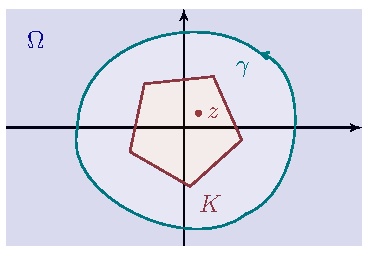
\includegraphics{Figuras/y para Gn'-Fn'.pdf}
       \end{figure}
       %
       Por hipótese, $F_n(z) \neq 0$ para todos $n\in\N$ e $z\in\Omega$, de modo
       que $F(z)\neq 0$ para todo $z\in\Omega$. Já que $F$ é holomorfa e, 
       consequentemente, contínua, podemos dizer que
       %
       \begin{equation*}
           \inf_{z\in K} |F(z)| = F(z_*) > 0.
       \end{equation*}
       %
       Portanto, podemos garantir que $G_n(z)$ é uniformemente limitada inferiormente
       em $n$ e $z\in K$. De fato,
       %
       \begin{align*}
           \inf_{z\in K} |G_n(z)| = \inf_{z\in K} |G_n(z) - F(z) + F(z)|
           \geq \inf_{z\in K} | |G_n(z) - F(z)| - |F(z)| |.
       \end{align*}
       %
       Como $G_n$ converge uniformemente para $F$, existe $n_0\in\N$ tal que
       se $n\geq n_0$, então 
       $|G_n(z) - F(z)| < \dis{\frac{1}{2} F(z_*) }$ para todo 
       $z\in K$. Logo, para todo $n\geq n_0$ temos
       %
       \begin{equation*}
           \inf_{z\in K} |G_n(z)| > \frac{1}{2}\inf_{z\in K} |F(z)| 
                                  = \frac{1}{2} F(z_*) > 0.
       \end{equation*}
       %
       Por outro lado, se $n\leq n_0$, então como $F_j(z)\neq 0$ para todo 
       $z\in\Omega$, temos que
       %
       \begin{align*}
           \inf_{z\in K} |G_n(z)| &= \inf_{z\in K} |F_1(z)|\cdots|F_n(z)| \\
                                  &\geq \prod_{j=1}^n \inf_{z\in K} |F_j(z)| \\
                                  &= |F_1(z^1_*)| \cdots |F_n(z^n_*)| \equiv I_K.
       \end{align*}
       %
       Portanto, 
       %
       \begin{equation*}
           \inf_{n\in\N} \inf_{z\in K} |G_n(z)| 
           \geq \min\left\{ I_K, \frac{1}{2}|F(z_*)| \right\} > 0,
       \end{equation*}
       %
       donde segue que 
       %
       \begin{equation*}
           \frac{G_n'}{G_n} \xrightarrow[\text{unif. em } K]{n\to\infty} \frac{F'}{F}
       \end{equation*}
       %
       para cada $z\in K$ e, como $K$ é compacto arbitrário, segue que
       %
       \begin{equation*}
           \frac{G_n'(z)}{G_n(z)} \xrightarrow{n\to\infty} \frac{F'(z)}{F(z)}
       \end{equation*}
       %
       para cada $z\in\Omega$. Observe que não podemos garantir que essa última
       convergência é uniforme em $\Omega$.
       
       Ademais, para cada $n\in\N$ temos
       %
       \begin{align*}
           \frac{G_n'(z)}{G_n(z)} 
           &= \frac{ \frac{d}{dz}[F_1(z)\cdots F_n(z)] }{F_1(z)\cdots F_n(z)} \\
           &= \sum_{j=1}^n F'_j(z)
           \frac{F_1(z)\cdots F_{j-1}(z)F_{j+1}(z)\cdots F_n(z)}{F_1(z)\cdots F_n(z)} 
           \\
           &= \sum_{j=1}^n \frac{F'_j(z)}{F_j(z)},
       \end{align*}
       %
       o que mostra que
       %
       \begin{equation*}
           \frac{F'(z)}{F(z)} = \lim_{n\to\infty} \frac{G'_n(z)}{G_n(z)}
                              = \lim_{n\to\infty} \sum_{j=1}^n \frac{F'_j(z)}{F_j(z)}
                              \equiv \sum_{j=1}^{\infty} \frac{F'_j(z)}{F_j(z)}.
       \end{equation*}
       %
    \end{proof}
    %
    
    Vamos usar este teorema para trabalhar com um exemplo interessante.
    \begin{exemplo}[A fórmula do produto da função seno]
    \index{Fórmula! do produto da função seno}
        Vamos estabelecer a validade da seguinte fórmula:
        %
        \begin{equation*}
            \frac{\sen(\pi z)}{\pi} = z\prod_{n=1}^{\infty} 
            \left( 1 - \frac{z^2}{n} \right).
        \end{equation*}
        %
        Para tanto, vamos estabelecer uma fórmula para $\cot(\pi z)$.
        Apesar de parecer estranha, a escolha da função cotangente é tudo menos
        coincidência. De fato, devido à Proposição \ref{prop:prod-inf-func-holom},
        para encontrar uma fórmula do produto da função $\sen(\pi z)/\pi$ precisaremos 
        considerar a sua derivada logarítmica, que nada mais é que $\pi\cot(\pi z)$.
        
        Vamos então mostrar que, para todo $z\in\C\setminus\mathbb{Z}$, temos
        %
        \begin{equation*}
            \pi\cot(\pi z) = \sum_{n=-\infty}^{\infty} \frac{1}{z+n}
                           \equiv \lim_{n\to\infty} \sum_{|j|\leq n} \frac{1}{z+j}
                           = \frac{1}{z} + \sum_{n=1}^{\infty} \frac{2z}{z^2 - n^2},
        \end{equation*}
        %
        onde usamos que
        %
        \begin{equation*}
            \frac{1}{z+n} + \frac{1}{z-n} = \frac{2z}{z^2 - n^2}.
        \end{equation*}
        %
        A estratégia para mostrar essa identidade será mostrar que tanto
        $F(z) = \pi\cot(\pi z)$ e $S(z) = \dis{\frac{1}{z} + 
        \sum_{n=1}^{\infty} \frac{2z}{z^2- n^2}}$ satisfazem as seguintes propriedades:
        %
        \begin{enumerate}[(i)]
            \item $H(z+1) = H(z)$;
            \item $H(z) = \dis{ \frac{1}{z} + H_0(z) }$, sendo $H_0$ analítica próxima
            do zero;
            \item $H(z)$ tem polos simples em $\Z$ e nenhuma outra singularidade.
        \end{enumerate}
        %
        De fato, para $F$,
        %
        \begin{enumerate}[(i)]
            \item 
            %
            \begin{align*}
                F(z+1)=\pi\cot(\pi(z+1)) &= \pi\frac{\cos(\pi(z+1))}{\sen(\pi(z+1))} \\
                                         &= \pi\frac{-\cos(\pi z)}{-\sen(\pi z)} \\
                                         &= \pi\cot(\pi z) \\
                                         &= F(z).
            \end{align*}
            %
            \item 
            %
            \begin{align*}
                \lim_{z\to 0} zF(z) &= \lim_{z\to 0} \pi z 
                \frac{\cos(\pi z)}{\sen(\pi z)} \\
                &= \lim_{z\to 0} \cos(\pi z)\cdot\frac{\pi z}{\sen(\pi z)} \\
                &= \lim_{z\to 0} \frac{\pi z}{\sen(\pi z)} \\
                &= 1 = \res(F,0).
            \end{align*}
            %
            Como $F$ tem apenas singularidades isoladas em $\Z$, segue do
            teorema de Laurent que para todo $z\in A(0,0,1)$ temos
            %
            \begin{equation*}
                F(z) = \frac{\res(F,0)}{z} + H_0(z) = \frac{1}{z} + H_0(z),
            \end{equation*}
            %
            com $H_0$ holomorfa em $D(0,1).$
            
            \item $F$ é claramente holomorfa em $\C\setminus\Z$.
        \end{enumerate}
        %
        Agora, para $S$, temos
        %
        \begin{enumerate}[(i)]
            \item $\forall z\in\C\setminus\Z$:
            %
            \begin{align*}
                S(z+1) &= \lim_{n\to\infty} \sum_{|j|\leq n} \frac{1}{z+1+j} \\
                       &= \lim_{n\to\infty}\left( \sum_{|j|\leq n+1} \frac{1}{z+j}
                       - \frac{1}{z-n-1} - \frac{1}{z-n} \right) \\
                       &= \lim_{n\to\infty} \sum_{|j|\leq n} \frac{1}{z_j} \\
                       &= S(z)
            \end{align*}
            %
            \item $\forall z\in D(0,1/2)$, temos
            %
            \begin{equation*}
                S(z) = \frac{1}{z} + \sum_{n=1}^{\infty} \frac{2z}{z^2 - n^2}.
            \end{equation*}
            %
            Considere a sequência de funções $h_n:D(0,1/2)\to\C$ dada por
            $h_n(z) = \dis{ \frac{2z}{z^2 - n^2} }$. Para cada $n\in\N$, temos
            que $h_n$ é uma função holomorfa e, além disso,
            %
            \begin{align*}
                \sup_{z\in D(0,1/2)} |h_n(z)| 
                = \sup_{z\in D(0,1/2)} \left| \frac{2z}{n^2
                \left( \frac{z^2}{n^2} - 1 \right)} \right|
                = \frac{2}{n^2}\sup_{z\in D(0,1/2)} 
                \frac{|z|}{\left| \frac{z^2}{n^2} - 1 \right|}
                = \frac{2}{n^2}.
            \end{align*}
            %
            Logo,
            %
            \begin{equation*}
                \sum_{n=1}^{\infty} \sup_{z\in D(0,1/2)} |h_n(z)|
                \leq 2\sum_{n=1}^{\infty} \frac{1}{n^2} < +\infty.
            \end{equation*}
            %
            Pelo teste M de Weierstrass, segue que 
            $\dis{ \sum_{n=1}^{\infty} h_n(z) \equiv S_0(z) }$ define uma função
            $S_0: D(0,1/2) \to\C$ holomorfa. Assim, 
            %
            \begin{equation*}
                S(z) = \frac{1}{z} + S_0(z),
            \end{equation*}
            %
            com $S_0$ holomorfa em $D(0,1/2)$.
            
            \item Fixado $n\in\Z$, temos que
            %
            \begin{align*}
                S(z) &= \frac{1}{z} + \sum_{j\in\N\setminus\{n\}} \frac{2z}{z^2 - j^2}
                + \frac{2z}{z^2 - n^2} \\
                &= S_1(z) + \frac{1}{z+n} + \frac{1}{z-n}.
            \end{align*}
            %
            Pelo teste M de Weierstrass, segue que $S_1(z) + \dis{\frac{1}{z+n}}$
            é holomorfa em $D(n, 1/2)$, de modo que $S$ tem apenas polos simples
            em cada ponto de $\Z$.
        \end{enumerate}
        %
        Sabendo que $F$ e $S$ satisfazem (i), (ii) e (iii), podemos afirmar que
        $H:\C\setminus\Z\to\C$ dada por
        %
        \begin{equation*}
            H(z) \equiv F(z) - S(z)
        \end{equation*}
        %
        satisfaz $H(z+1) = H(z)$. Ademais, segue da propriedade (ii) que
        $\res(H,0) = 0$, de modo que $z=0$ é uma singularidade removível de $H$.
        Esta informação, junto com a periodicidade de $H$ dada pelo item (i)
        implica que, para todo $n\in\Z$,
        %
        \begin{equation*}
            \lim_{z\to n} H(z) = \lim_{z\to n} H(z-n) = \lim_{z\to 0} H(z) = 0.
        \end{equation*}
        %
        Logo, segue do teorema de Riemann que $H$ admite extensão inteira.
        
        Para estabelecer a fórmula da cotangente, é suficiente mostrar que
        $H$ é limitada e usar o teorema de Liouville.
        
        Ademais, para mostrar que $H$ é limitada, basta trabalhar na faixa
        %
        \begin{equation*}
            S_{\frac{1}{2}} = \left\{ z\in\C : |\Re(z)| \leq \frac{1}{2} \right\},
        \end{equation*}
        %
        uma vez que $H$ satisfaz a periodicidade (i).
        %
        \begin{figure}[H]\centering
            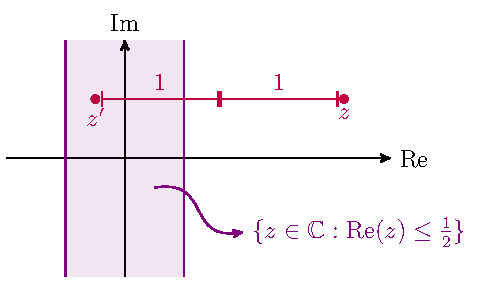
\includegraphics{Figuras/S_meio.pdf}
        \end{figure}
        %
        Já que $H:\C\to\C$ é inteira, então $H$ é limitada em
        %
        \begin{equation*}
            \Omega_1 = S_1 \cap S_{\frac{1}{2}},
        \end{equation*}
        %
        com
        %
        \begin{equation*}
            S_1 = \{ z\in\C : |\Im(z)| \leq 1 \},
        \end{equation*}
        %
        ou seja, 
        %
        \begin{equation}
            \sup_{z\in \Omega_1} |H(z)| = k_1 < +\infty
        \end{equation}
        %
        pois $\Omega_1$ é um compacto, como ilustrado abaixo.
        %
        \begin{figure}[H]\centering
            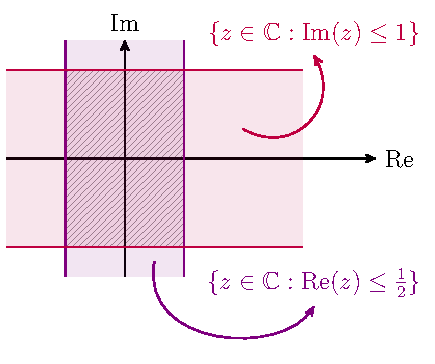
\includegraphics{Figuras/S_meio cap S_1.pdf}
            \caption{%
                A região hachurada, $\Omega_1$, é um compacto.
            }
        \end{figure}
        %
        Para terminar a demonstração que $H$ é limitada em $S_{\frac{1}{2}}$,
        resta analisar o que acontece com a função em
        %
        \begin{equation*}
            \Omega_2 = S_{\frac{1}{2}} \cap \left\{ z\in\C : |\Im(z)| > 1 \right\}.
        \end{equation*}
        %
        Ora, se $z = x + iy$, então
        %
        \begin{align*}
            \cot(\pi z) &= 
            i\frac{ e^{i\pi z} + e^{-i\pi z} }{ e^{i\pi z} - e^{-i\pi z} } \\
            &= i\frac{ e^{i\pi x}e^{-\pi y} + e^{-i\pi x}e^{\pi y} }
            { e^{i\pi x}e^{-\pi y} - e^{-i\pi x}e^{\pi y} } \\
            &= i\frac{ e^{-2\pi y} + e^{-2\pi ix} }{ e^{-2\pi y} - e^{-2\pi ix} }.
        \end{align*}
        %
        Como estamos supondo $|y|>1$, segue que
        %
        \begin{align*}
            |\cot(\pi z)| = 
            \left| 
            \frac{ e^{-2\pi y} + e^{-2\pi ix} }{ e^{-2\pi y} - e^{-2\pi ix} } 
            \right|
            \leq \frac{ 1 + e^{-2\pi y} }{ 1 - e^{-2\pi y} }
            \leq \widetilde{k_1}.
        \end{align*}
        %
        Ainda para $|y|>1$ e $|x|\leq 1/2$, temos
        %
        \begin{align*}
            \left| 
            \frac{1}{z} + \sum_{n=1}^{\infty} \frac{2z}{z^2 - n^2} 
            \right|
            &= \left| 
            \frac{1}{x+iy} + \sum_{n=1}^{\infty} \frac{2(x+iy)}{x^2 - y^2 - n^2 +2ixy} 
            \right| \\
            &\leq \frac{1}{\sqrt{x^2 + y^2}} 
            + \sum_{n=1}^{\infty} \frac{|2x|}{\sqrt{(x^2 - y^2 - n^2)^2 + 4x^2y^2}} \\
            &+ \sum_{n=1}^{\infty} \frac{|2y|}{\sqrt{(x^2 - y^2 - n^2)^2 + 4x^2y^2}} \\
            &\leq 1 
            + \sum_{n=1}^{\infty} \frac{1}{|y|^2 + n^2 - 1/4}
            + \sum_{n=1}^{\infty} \frac{|2y|}{|y|^2 + n^2 - 1/4} \\
            &\leq 1 + \sum_{n=1}^{\infty} \frac{1}{n^2} 
            + 2\sum_{n=1}^{\infty} \frac{|y|}{|y|^2/4 + n^2 - n^2/4} \\
            &\leq 1 + \frac{\pi^2}{6} + 
            8\sum_{n=1}^{\infty} \frac{|y|}{\frac{1}{4}(|y|^2 + 3n^2)} \\
            &\leq 1 + \frac{\pi^2}{6} +
            8\sum_{n=1}^{\infty} \frac{|y|}{|y|^2 + n^2}.
        \end{align*}
        %
        Agora, como $b:(0, +\infty)\to\R$ dada por $\dis{ b(x) = \frac{|y|}{|y|^2 + x^2} }$
        é decrescente já que
        %
        \begin{equation*}
            b'(x) = |y|\frac{-2x}{(|y|^2 + x^2)^2} < 0 \, \forall x+iy \in\Omega_2,
        \end{equation*}
        %
        podemos assegurar que
        %
        \begin{equation*}
            \sum_{n=1}^{\infty} \frac{|y|}{|y|^2 + n^2} 
            \leq
            \int_0^{\infty} \frac{|y|}{|y|^2 + x^2} \, dx.
        \end{equation*}
        %
        \begin{figure}[H]\centering
            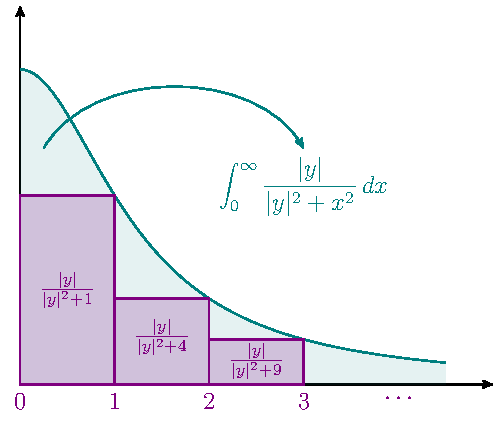
\includegraphics{%
                Figuras/majoração por integral.pdf
            }
        \end{figure}
        %
        Agora, considerando a mudança de variáveis $u = x/|y|$, temos
        %
        \begin{align*}
            \int_0^{\infty} \frac{|y|}{|y|^2 + x^2} \, dx = 
            \int_0^{\infty} \frac{1}{1 + u^2} \, du =
            \frac{\pi}{2}.
        \end{align*}
        %
        Até o momento, mostramos que
        %
        \begin{enumerate}
            \item $|\cot(\pi z)| = \dis{ 
            \left|\frac{ e^{-2\pi y} + e^{-2i\pi x} }{ e^{-2\pi y} - e^{-2i\pi x} } \right|
            \leq \frac{ 1 + e^{-2\pi y} }{ 1 - e^{-2\pi y} }
            \leq \widetilde{k_1}}$;
            
            \item $|S(z)| = \dis{ 
            \left| \frac{1}{z} + \sum_{n=1}^{\infty} \frac{2z}{z^2 - n^2} \right| 
            \leq 1 + \frac{\pi^2}{6} + 8\int_0^{\infty} \frac{|y|}{|y|^2 + x^2} \, dx
            = 1 + \frac{\pi^2}{6} + 4\pi =
            \widetilde{k_2}}$,
        \end{enumerate}
        %
        donde segue que
        %
        \begin{align*}
            \sup_{z\in\Omega_2} |H(z)| \leq 
            \sup_{z\in\Omega_2} |F(z) - S(z)| \leq
            \pi\widetilde{k_1} + \widetilde{k_2} \equiv
            k.
        \end{align*}
        %
        Portanto, lembrando que $H$ é periódica, temos
        %
        \begin{equation*}
            \sup_{z\in\C} |H(z)| =
            \sup_{z\in\Omega_1\cup\Omega_2} |H(z)| \leq
            k,
        \end{equation*}
        %
        ou seja, $H$ é limitada em $\C$.
        Pelo teorema de Liouville, como $H$ é inteira, temos
        $H(z)$ constante. 
        Agora, note que $H$ pode ser vista como extensão holomorfa de $F(z) - S(z)$,
        que é uma função ímpar. Portanto, $H$ 
        também é ímpar e $H(0) = 0$, donde segue 
        que $H\equiv 0$, ou seja, $F(z) \equiv S(z)$ e temos
        %
        \begin{equation*}
            \pi\cot(\pi z) = \frac{1}{z} + \sum_{n=1}^{\infty} \frac{2z}{z^2 - n^2},
            \, \forall z\in\C\setminus\Z.
        \end{equation*}
        %
        Finalmente, para mostrar a fórmula de produto para o seno, sejam
        %
        \begin{align*}
            G(z) &= \frac{\sen(\pi z)}{\pi} , \\
            P(z) &= z\prod_{n=1}^{\infty} \left( 1 - \frac{z^2}{n^2} \right).
        \end{align*}
        %
        Para mostrar a convergência de $P(z)$, vamos usar a 
        Proposição \ref{prop:prod-inf-func-holom} com $P(z) = zF(z)$, 
        $\Omega = D(0,R)\setminus\Z$,
        $F_n(z) = 1 - \dis{ \frac{z^2}{n^2} }$. Daí, temos
        %
        \begin{equation*}
            |F_n(z) - 1| \leq \sup_{z\in\Omega} \frac{|z|^2}{n^2} = \frac{R^2}{n^2}
            \equiv c_n.
        \end{equation*}
        %
        Portanto, para todo $z\in\Omega$,
        %
        \begin{align*}
            \frac{P'(z)}{P(z)} =
            \frac{1}{z} + \sum_{n=1}^{\infty} \frac{ -\frac{2z}{n^2} }{ 1 - \frac{z^2}{n^2} }
            = \frac{1}{z} + \sum_{n=1}^{\infty} \frac{2z}{z^2 - n^2}.
        \end{align*}
        %
        Agora, como $G'(z)/G(z) = \pi\cot(\pi z)$, 
        o resultado que acabamos de mostrar
        nos dá, para todo $z\in\Omega$,
        %
        \begin{equation*}
            \left( \frac{P(z)}{G(z)} \right)'
            = \frac{ P'(z)G(z) - P(z)G'(z) }{ G^2(z) }
            = \frac{P(z)}{G(z)}\left[ \frac{P'(z)}{P(z)} - \frac{G'(z)}{G(z)} \right]
            \equiv 0,
        \end{equation*}
        %
        de modo que $P(z) = cG(z)$ para alguma constante $c, \, \forall z\in\Omega$,
        pois $\Omega$ é conexo. 
        Ora, então
        %
        \begin{equation*}
            1 
            = \lim_{z\to 0} \prod_{n=1}^{\infty} \left( 1 - \frac{z^2}{n^2} \right)
            = \lim_{z\to 0} \frac{P(z)}{z} 
            = c\lim_{z\to 0} \frac{G(z)}{z}
            = c\lim_{z\to 0} \frac{\sen(\pi z)}{\pi z}
            = c,
        \end{equation*}
        %
        onde usamos que o produtório é holomorfo.
        Portanto, $P(z) = G(z)$ para todo $z\in\Omega$. 
        Pelo Princípio da Identidade,
        como $\Omega$ é aberto e conexo, segue que essa identidade vale para todo
        $z\in\C$.
    \end{exemplo}
    %
    \begin{exercicio}
        Use a série de Taylor de $\sin z$ e a identidade 
        % 
        \[
          \sin \pi z = \pi z\prod_{n=1}^\infty \left(1 - \frac{z^2}{n^2}\right),
        \]
        %
        deduzida acima, para demonstrar que 
        %
        \[
          \sum_{n=1}^\infty \frac{1}{n^2} = \frac{\pi^2}{6}.
        \]
    \end{exercicio}
    %
    
\section{O Teorema de Weierstrass}
    
    Anteriormente, vimos que, para construir uma função com zeros prescritos 
    na forma de uma lista ou sequência $\{a_n\}$, 
    uma tentativa ingênua era escrever
    %
    $$ f(z) = \lim_{n \to \infty} (z-a_1) \cdots (z-a_n).$$
    %
    Produtos como esse (em geral) não convergem para qualquer sequência 
    escolhida $\{a_n\}$, então essa não é a melhor escolha para construir $f$. 
    
    Mostramos, também, que vale a igualdade 
    %
    $$\frac{\sin{\pi z}}{\pi} = z \prod_{n = 1}^{\infty} \left(1 - \frac{z^2}{n^2}\right)$$
    %
    e a função $\sin{\pi z}$ se anula exatamente em $\mathbb{Z}$. 
    Analisando o produto com mais cuidado, vemos que cada fator é da forma 
    $(n^2 - z^2)/n^2 = (n - z)(n + z)/n^2$ 
    que se anula exatamente em $\pm n \in \Z$. 
    Além disso, o fato de termos escolhido fatores 
    %
    $$\left(1 - \frac{z^2}{n^2}\right)$$
    %
    em vez de $(n^2 - z^2)$ 
    nos permitiu usar a Proposição \ref{prop:prod-inf-func-holom}. 
    
    Se queremos definir uma função que se anula precisamente em uma sequência 
    qualquer $\{a_n\}$ de uma forma análoga à vista acima, ter $z^2$ nos 
    fatores pode não ser vantajoso, pois $-a_n$ pode não estar na sequência e mesmo 
    assim anular a função se $a_n$ anulá-la. Ademais, o fator $z^2$ não teve nenhuma 
    importância particular em termos de estimativas a nosso favor. Portanto, um bom 
    caminho é considerar fatores da forma
    %
    $$ \left(1 - \frac{z}{a_n}\right)g_n(z), $$
    %
    onde $g_n(z)$ são funções que facilitariam a convergência. O grande problema 
    está em como escolher tais funções e é neste ponto que reside a maior 
    contribuição de Weierstrass: ele encontrou funções que garantem a 
    convergência dada qualquer sequência $\{a_n\}$.
    
    Vamos enunciar o grande resultado desta seção agora 
    e demonstrá-lo no decorrer do texto.
    
    \begin{teorema}[Teorema do Produto de Weierstrass]
    \label{teo-Weierstrass-fatoracao}
    \index{Teorema!do Produto de Weierstrass}
        Dada uma sequência $\{a_n\}$ de números complexos tal que 
        $|a_n| \to \infty$, quando $n \to \infty$, 
        existe uma função inteira $f: \C \to \C$ que 
        se anula em $z=a_n$, para cada $n\in\mathbb{N}$, 
        e não se anula em quaisquer outros pontos do plano complexo.
        
        Além do mais, se $a_m\neq a_n$ 
        para todo $m\neq n$, então, para 
        cada $n\in\N$ temos que $z=a_n$ 
        é um zero simples de $f$ (multiplicidade um). 
    \end{teorema}
 
 \bigskip 
    
    Note que não é possível existir uma função como no enunciado do Teorema
    de Weierstrass, quando a sequência $\{a_n\}$ 
    assume infinitos valores distintos e
    a condição $|a_n| \xrightarrow{n\to\infty} \infty$ não é satisfeita.
    De fato, suponha por absurdo que exista tal função. 
    Já que $\{a_n\}$ toma infinitos valores distintos e 
    a sequência $|a_n|$ não tende a infinto, quando $n\to \infty$,
    podemos encontrar algum $R>0$ e infinitos elementos distintos 
    da sequência $\{a_n\}$ dentro do disco fechado $\overline{D(0,R)}$. 
    Desta forma, segue da compacidade de $\overline{D(0,R)}$, 
    que existe alguma 
    subsequência $\{a_{n_{k}}\}$ de $\{a_n\}$, formada também
    por elementos distintos, que converge
    para algum ponto $w\in \overline{D(0,R)}$.
    Isto é, $a_{n_{k}}\to w$, quando $k\to\infty$.
    Como $f(a_{n_{k}})=0$, para  todo $k\in\mathbb{N}$ 
    e $f$ é contínua, então segue que 
    $f(w)=f(\lim_{k\to\infty} a_{n_k})=\lim_{k\to\infty} f(a_{n_k}) =0$.  
    Logo $w$ é um zero de $f$ que é um ponto aderente à uma 
    sequência de zeros de $f$. Portanto segue do Princípio da Identidade 
    que $f\equiv 0$. Mas isto é um absurdo, pois estamos assumindo 
    que $a_1, a_2, \dots$ são os únicos zeros de $f$.
 
 
 \bigskip 
 
    
    Vamos introduzir agora um dos ingredientes mais importantes da prova
    do Teorema de Weierstrass, que são os chamados fatores canônicos. 
    Para cada $k \in \N$, definimos 
    o fator canônico de grau $k$ por
    \index{Fatores Canônicos}
    %
    \[
    E_k(z) = (1-z)\exp{\left(z + \frac{z^2}{2} + \cdots + \frac{z^k}{k}\right)}.
    \]
    %
    Para $k=0$, definimos $E_0(z) = 1-z$ Observe que a 
    função $E_k(z/w)$ se anula apenas em $z = w$ (se $w \neq 0$). 
    %
    \begin{lema}
    \label{lema-wstr-est-factor}
    Se $|z| \leq 1/2$, então, para algum $c>0$, 
    temos $|1-E_k(z)| \leq c|z|^{k+1}$ qualquer 
    que seja $k$ inteiro não negativo.
    \end{lema}
    %
    \begin{proof}
    Podemos escolher um ramo do logaritmo adequado 
    de modo que vale a equação $1-z = \exp{\log(1-z)}$. 
    Além disso, da série geométrica, sabemos que 
    %
    \[
    \frac{1}{1-z} = \sum_{n=0}^{\infty}z^n 
    \]
    %
    já que $|z| \leq 1/2 < 1$. Integrando esta equação, obtemos que
    %
    \[ 
    \log(1-z) = - \sum_{n=0}^{\infty}\frac{z^n}{n}.
    \]
    %
    Observe que 
    %
    \begin{align*}
        E_k(z) &= \exp{\left(\log(1-z) + z + \cdots + \frac{z^k}{k}\right)} \\
        &= \exp\left(-\sum_{n=k+1}^{\infty}\frac{z^n}{n}\right) \\
        &= \exp{w}.
    \end{align*}
    %
    Agora, estimamos $|w|$:
    %
    \begin{align*}
        |w| &= \left | -\sum_{n=k+1}^{\infty}\frac{z^n}{n} \right | \\
        &\leq |z|^{k+1}\sum_{n=k+1}^{\infty}\frac{|z|^{n - (k+1)}}{n} \\
        &\leq |z|^{k+1}\sum_{n=0}^{\infty}|z|^n \\
        &\leq |z|^{k+1}\sum_{n=0}^{\infty} 2^{-n} \\
        &= 2|z|^{k+1} \leq 2 \frac{1}{2^{k+1}} \leq 1.
    \end{align*}
    %
    Portanto,
    %
    \begin{align*}
        |1 - E_k(z)| = |1 - \exp{w}| 
        &= \left | \sum_{n=1}^{\infty}\frac{w^n}{n!} \right | \\
        &\leq |w|\sum_{n=1}^{\infty}\frac{|w|^{n-1}}{n\cdot (n-1)!} \\
        &\leq |w|\sum_{n=0}^{\infty}\frac{|w|^n}{n!} \\
        &\leq |w|\sum_{n=0}^{\infty}\frac{1}{n!} \\
        &=|w|e \leq 2e|z|^{k+1}.
    \end{align*}
    %
    Tomando $c = 2e$, temos o resultado.
    \end{proof}
    %
    
    Observe que, neste lema, a escolha $|z| \leq 1/2$ é 
    feita por motivos de simplicidade. Em termos práticos 
    poderíamos escolher $|z| \leq \alpha$ para $\alpha \in (0,1)$.
    
    Dada uma função inteira $f$, se $a$ é um zero de ordem 
    $m$ de $f$, então existe uma função inteira $g$ tal que
    %
    \[ 
    f(z) = (z-a)^mg(z) 
    \]
    %
    e $g(a) \neq 0$. Portanto, para os nossos propósitos, 
    podemos supor que a sequência de zeros no Teorema de 
    Weierstrass não contém o zero. Vamos mostrar que função 
    %
    \[ 
    f(z) = z^m \prod_{n=1}^{\infty}E_n(z/a_n)
    \]
    %
    tem um zero de ordem $m$ na  origem e se anula em $a_n$ 
    para todo $n$ e em nenhum outro ponto.
    
    Seja $R>1$ e denote $D_R = D(0,R)$. Existe $n_0 \in \N$ tal que 
    %
    \begin{align*}
        \begin{cases}
            |a_n| < 2R, \text{ se } n \leq n_0 \\
            |a_n| \geq 2R, \text{ se } n > n_0
        \end{cases},
    \end{align*}
    %
    pois supomos que $|a_n| \to \infty$. Note que a função 
    %
    \[
    z^m\prod_{n=1}^{n_0}E_n(z/a_n)
    \]
    %
    é inteira e se anula precisamente em $z = 0$ e $z = a_n$ com 
    $n \leq n_0$. Para $n > n_0$, temos $|a_n| \geq 2R$ e segue que
    %
    \[
    \left | \frac{z}{a_n} \right | \leq \frac{|z|}{2R} < \frac{R}{2R} = \frac{1}{2}
    \]
    %
    sempre que $|z| < R$. Do Lema \ref{lema-wstr-est-factor} 
    concluímos que 
    $|1 - E_n(z/a_n)| \leq c|z/a_n|^{n+1} \leq c2^{-(n+1)}$ 
    para $z \in D_R$ e $n > n_0$. 
    Pela Proposição \ref{prop:prod-inf-func-holom}, concluímos que 
    %
    \[
    \prod_{n=n_0 + 1}^{\infty}E_n(z/a_n)
    \]
    %
    converge uniformemente em $D_R$ para uma função holomorfa 
    e que não se anula em $D_R$.
    
    Para cada $R$, concluímos que a função 
    %
    \[
    f_R (z) = z^m\left(\prod_{n=1}^{n_0}E_n(z/a_n)\right)\left(\prod_{n=n_0 + 1}^{\infty}E_n(z/a_n)\right)
    \]
    %
    é holomorfa em $D_R$ e se anula precisamente em $z = 0$ 
    e nos pontos da sequência $\{a_n\}$ no interior de $D_R$. 
    Podemos reescrever a expressão acima numa forma mais conveniente:
    %
    \begin{align*}
        f_R (z) &= z^m \cdot \prod_{n=1}^{n_0}E_n(z/a_n) \cdot \lim_{N \to \infty}\prod_{n=n_0 + 1}^{N}E_n(z/a_n) \\
        &= \lim_{N \to \infty} \left( z^m \cdot \prod_{n=1}^{n_0}E_n(z/a_n) \right) \cdot \prod_{n=n_0 + 1}^{N}E_n(z/a_n) \\
        &= \lim_{N \to \infty}  z^m \cdot \prod_{n=1}^{N}E_n(z/a_n) \\
        &= z^m \prod_{n=1}^{\infty}E_n(z/a_n).
    \end{align*}
    %
    Por construção, é simples ver que, se $R'>R$, então 
    $f_{R'}|_{D_R} = f_R$, ou seja, $f_{R'}$ 
    é uma extensão analítica de $f_R$. Isto mostra que a aplicação
    %
    \[
    z \mapsto z^m \prod_{n=1}^{\infty}E_n(z/a_n)
    \]
    %
    está bem definida para todo $z \in \C$, pois $R$ é arbitrário 
    e define uma função que satisfaz as conclusões do Teorema de Weierstrass.
    
    A força deste teorema pode ser vista por uma consideração simples. 
    Como saber se um produtório da forma
    %
    $$\prod_{n=1}^{\infty} \left( 1 - \frac{z}{a_n} \right)$$
    %
    converge? Pela Proposição \ref{prop:prod-inf-func-holom}, 
    um caminho seria analisar se a soma 
    %
    \[
    \sum_{n=1}^{\infty} \left | \frac{z}{a_n} \right |
    \]
    %
    converge ou não. Isto naturalmente impõe condições sobre a sequência em questão. 
    Utilizando o que foi construído no Teorema de Weierstrass, 
    podemos considerar sequências arbitrárias. Uma consequência disso é que, 
    além dos zeros, podemos escolher suas multiplicidades, 
    já que um mesmo valor pode se repetir na sequência.
    %
    \begin{corolario}
    Se duas funções $f_1$ e $f_2$ satisfazem as 
    condições do Teorema de Weierstrass, então $f_1(z) = f_2(z)\exp{g(z)}$ 
    para alguma função inteira $g(z)$. 
    \end{corolario}
    %
    \begin{observacao}
        O corolário acima é essencialmente a solução ao seguinte problema:
        dada $f_2$ inteira, como obter $f_1$ 
        inteira e com os mesmos zeros de $f_2$?
        Um raciocínio heurístico que nos ajuda a 
        esclarecer a resposta é o seguinte:
        atendendo à preservação dos zeros, 
        é claro que não se pode fazer sobre $f_2$ 
        operações como translação e inversão, e intuitivamente 
        ficamos mesmo só com operações de rotação e 
        expansão (ou contração), que podem ser executadas 
        simultaneamente pela exponencial complexa.
        Finalmente, $f_1$ ser inteira pede que o 
        argumento da exponencial também seja inteiro, 
        e portanto $f_1=f_2\cdot\exp\circ g$ para alguma $g$ inteira.
    \end{observacao}
    %
    \begin{proof}
    Seja $h(z) = f_1(z)/f_2(z)$. Se $f_1$ e $f_2$ 
    ambas se anulam em um ponto $a$, 
    então este é um zero de mesma multiplicidade para ambas, 
    ou seja, $f_i(z) = (z-a)^mg_i(z)$ com $g_i$ holomorfa e 
    $g_i(a) \neq 0$ para  $i = 1,2$ e $m$ natural. 
    
    Tomando o limite de $h(z)$ quando $z \to a$, 
    vemos que o limite existe e é não nulo, logo, 
    $a$ é uma singularidade removível de $h$, então podemos estender $h$ 
    para todo o plano complexo fazendo 
    $h(a) = \lim_{z \to a} h(z)$ para cada singularidade $a$.
    
    Usando a mesma notação para $h$ e sua extensão, temos que ela é inteira. 
    Como $\C$ é simplesmente conexo, 
    segue do Lema \ref{lema-ramo-log} que $h(z) = \exp{g(z)}$ 
    para alguma função $g$ inteira.
    \end{proof}
    %
    
    \subsection{Interpolações e o Teorema de Weierstrass}
    
    
    Nesta seção vamos apresentar uma aplicação muito 
    interessante do Teorema de Weierstrass. 
    Ela é baseada também em outro importante teorema, 
    conhecido como Teorema de Mittag-Leffler 
    (veja abaixo, Teorema \ref{teo-mittag-leffler}). 
    
    
    Um dos problemas mais clássicos de 
    interpolação polinomial consiste em: 
    fornecido um conjunto finito de pares 
    de números complexos (ou reais) da forma
    %
    \[
    (z_1,w_1), (z_2,w_2), \ldots, (z_n,w_n);
    \]
    %
    encontrar um polinômio $P$ de menor grau possível 
    cujo gráfico contém todos estes pares de pontos, 
    ou seja, $P(z_j)=w_j$ para cada $j=1,\ldots,n$. 
    Às vezes, nos referimos a um polinômio 
    satisfazendo esta propriedade como um 
    polinômio interpolador\index{Polinômio! interpolador} e os pares de
    números complexos $(z_i,w_i)$, com $i=1,\ldots,n$ como dados.
    
    Caso o conjunto de dados acima não possua nenhuma propriedade especial, em geral, um 
    polinômio interpolador para estes dados 
    terá grau no mínimo $n-1$. 
    Na verdade, Lagrange mostrou
    que este problema sempre 
    admite uma solução com um polinômio de grau exatamente $n-1$. 
    Tais polinômios são chamados, hoje em dia, 
    de polinômios interpoladores de Lagrange\index{Polinômio! interpolador de Lagrange}. 
    Para o conjunto de dados fornecidos acima, 
    o polinômio interpolador de Lagrange tem a forma 
    %
    \[
      P(z)
      =
      \sum_{k=1}^n 
      w_k
      \prod_{\substack{j=1 \\ j\neq k}}^n
      \frac{z-z_j}{z_k-z_j}
    %   \frac
    %   {(z-z_1)(z-z_2)\cdots (z-z_{j-1})(z-z_{j+1})\cdots (z-z_n)}
    %   {(z_j-z_1)(z_j-z_2)\cdots (z_j-z_{j-1})(z_j-z_{j+1})\cdots (z_j-z_n)}
    \]
    %
    
    No que segue, usamos os Teoremas 
    de Weierstrass e Mittag-Leffler para mostrar que dada
    uma sequência infinita de números complexos 
    distintos $(z_n)_{n\in\N}$ e uma sequência arbitrária
    $(w_n)_{n\in\N}$, se $|z_n|\xrightarrow{n\to\infty}\infty$, 
    então podemos construir uma
    função inteira $f:\C\to\C$ tal que 
    $f(z_n)=w_n$, para todo $n\in\mathbb{N}$.
    Note que esta aplicação pode ser vista 
    como um resultado de interpolação e que, na verdade, 
    generaliza o esquema de interpolação baseado nos 
    polinômios de Lagrange, mas
    para o caso de uma interpolação 
    em que a função deve se ajustar a um 
    conjunto infinito enumerável de valores. 
    
    Como mencionado acima, para resolver o problema 
    de interpolação, por uma função inteira, 
    de um conjunto infinito de dados, vamos
    precisar do Teorema de Mittag-Leffler. Este é um resultado
    de natureza análoga à do Teorema de Weierstrass, 
    mas que ao invés de considerar o problema de zeros prescritos,
    considera o problema de existência de uma 
    função meromorfa
    em $\C$ cujas singularidades são 
    polos de ordem e localização prescritos por 
    alguma sequência de números complexos 
    $(z_n)$ satisfazendo $|z_n|\xrightarrow{n\to\infty}\infty$.
    
    
    \begin{teorema}[Teorema de Mittag-Leffler]
    \label{teo-mittag-leffler}
    \index{Teorema!de Mittag-Leffler}
    Seja $(z_n)_{n\in\mathbb{N}}$ uma 
    sequência de número complexos distintos com 
    $|z_n|\xrightarrow{n\to\infty}\infty$. 
    Seja $(P_n)_{n\in\N}$ uma sequência qualquer de polinômios 
    não-nulos tais que $P_n(0)=0$, 
    para todo $n\in\N$. 
    Então existe uma função $f$ meromorfa em 
    $\C$ cujas singularidades são apenas os pontos da sequência $(z_n)_{n\in\N}$ e a parte
    principal da série de Laurent de $f$ em torno de
    $z_n$ é dada exatamente por $P_n\big(1/(z-z_n)\big)$,
    isto é, para cada $n\in\N$, 
    existe um raio positivo $r_n$ dado por
    $r_n \equiv \inf\{|z_n-z_j|: j\in \N\setminus\{n\} \}$ 
    tal que para todo ponto $z$ 
    do anel aberto $A(z_n,0,r_n)$ temos
    %
    \[
    f(z) = P_n\left(\frac{1}{z-z_n}\right)+h_n(z),
    \]
    %
    onde $h_n:D(z_n,r_n)\to\C$ é uma função holomorfa.
    \end{teorema}
    
    
    A maneira mais natural de pensar em como este teorema 
    poderia ser provado  seria
    considerando a seguinte série de funções: 
    \[
     f(z) = \sum_{n=1}^{\infty} P_n\left( \frac{1}{z-z_n}  \right).
    \]
    Entretanto, como o leitor já deve estar imaginando, 
    esta tentativa esbarraria no problema
    da convergência desta série, 
    já que no enunciado do teorema é permitido escolher 
    a sequência  $(z_n)_{n\in\N}$ de forma muito geral. 
    Não obstante, veremos que a prova é baseada nesta ideia:
    ao invés de considerarmos exatamente esta série, 
    vamos construir uma outra série de funções que 
    é basicamente uma modificação da série acima, onde 
    cada parcela desta nova série é obtida
    subtraindo-se uma função holomorfa apropriada 
    de cada uma das parcelas da série acima. 
    
    
    
    
    \begin{proof}[Prova do Teorema de Mittag-Leffler]
    Primeiro vamos assumir que $z_n\neq 0$, para todo $n\in\N$.
    Desta forma 
    $U\equiv \C\setminus\{z_1,z_2,\ldots\}$ 
    é um domínio contendo a origem do plano complexo.
    
    
    Para cada $n\in\N$, temos que a função $g_n:U\to\mathbb{C}$
    dada por
    %
    \[
    g_n(z) = P_n\left(\frac{1}{z-z_n}\right),
    \]
    %
    define uma função analítica em $U$. 
    Observe que a única singularidade de 
    $g_n$ é o ponto $z=z_n$. 
    Portanto, podemos garantir para todo $z\in D(0,|z_n|)$ que
    %
    \[
    g_n(z) = \sum_{k=0}^{\infty} \frac{g_{n}^{(k)}(0)}{k!}z^k. 
    \]
    %
    Além do mais, para cada $n\in\N$, existe $k_n\in\mathbb{N}$ tal que
    %
    \begin{equation}
    \label{eq-aux1-teo-mittag-leffer}
    \left| 
    g_n(z) - \sum_{k=0}^{k_n} \frac{g_{n}^{(k)}(0)}{k!}z^k
    \right|
    =
    \left| 
    \sum_{k=k_n+1}^{\infty} \frac{g_{n}^{(k)}(0)}{k!}z^k
    \right|
    \leq 
    \frac{1}{2^n},\quad \forall z\in \overline{D(0,|z_n|/2)}.
    \end{equation}    
    %
    Para cada $n\in\N$, considere a função $f_n:U\to\C$ dada por
    %
    \[
    f_n(z) = P_n\left(\frac{1}{z-z_n}\right)- \sum_{k=0}^{k_n} \frac{g_{n}^{(k)}(0)}{k!}z^k.
    \]
    %
    Claramente $f_n$ é uma função holomorfa em $U$. 
    
    O próximo passo é mostrar que a função $f$ dada
    pela seguinte série de funções 
    %
    \[
    f\equiv \sum_{n=1}^{\infty} f_n
    \]
    %
    está bem definida em $U$ e, além disso, define uma
    função holomorfa neste domínio. 
    Para provar estas afirmações a ideia é 
    usar o Teste M de Weierstrass. 
    
    Seja $K\subset U$ um subconjunto compacto arbitrário. 
    Como $|z_n|\xrightarrow{n\to\infty}\infty$, podemos 
    garantir que existe algum 
    $n_0\in\N$ tal que $K\subset \overline{D(0,|z_n|/2)}$ 
    para todo $n\geqslant n_0$. 
    
    Usando a desigualdade \eqref{eq-aux1-teo-mittag-leffer}
    e as observações acima, podemos garantir que
    %
    \[
    \sum_{n=n_0}^{\infty} \sup_{z\in K}|f_n(z)|
    \leqslant 
    \sum_{n=n_0}^{\infty} \sup_{z\in \overline{D(0,|z_n|/2)}} |f_n(z)|
    \leqslant 
    \sum_{n=n_0}^{\infty} \frac{1}{2^n}
    \leqslant
    2.
    \]
    %
    Logo, segue da continuidade das $f_j$'s em $K$ 
    e da desigualdade acima que
    %
    \[
    \sum_{n=1}^{\infty} \sup_{z\in K} |f_n(z)|
    \leqslant
    \sum_{n=1}^{n_0} \sup_{z\in K} |f_n(z)|
    +2
    <+\infty.
    \]
    %
    Como $K$ é um subconjunto arbitrário de $U$, segue do teste
    M de Weierstrass que a série de funções 
    $\sum_{n=1}^{\infty}f_n$ define uma função holomorfa em $U$,
    que denotaremos por $f$. 
    
    Para finalizar a prova do Teorema,
    precisamos obter a série de Laurent de $f$ 
    em torno de cada uma de suas singularidades.
    
    Para cada $n\in\mathbb{N}$, seja 
    $r_n \equiv \inf\{ |z_n-z_j|: j\in\N\setminus\{n\}\}$. 
    Considere a função $q_n:A(z_n,0,r_n)\to\C$ dada por
    %
    \[
    q_n(z) = f(z)-f_n(z) \equiv 
    f(z)- P_n\left(\frac{1}{z-z_n}\right) +
    \sum_{k=0}^{k_n} \frac{g_{n}^{(k)}(0)}{k!}z^k.
    \]
    %
    Para finalizar a prova, basta mostrar 
    que $z_n$ é a única singularidade
    da função $q_n$ em $D(z_n,r_n)$ 
    e que esta singularidade 
    é removível, pois já
    que $P_j(0)=0$, para todo $j\in\N$,
    podemos obter, imediatamente, da identidade abaixo
    %
    \[
    f(z) = P_n\left(\frac{1}{z-z_n}\right) + q_n(z)+
    \sum_{k=0}^{k_n} \frac{g_{n}^{(k)}(0)}{k!}z^k
    \]
    %
    que $P_n(1/(z-z_n))$ é a parte principal da 
    série de Laurent de $f$ no anel $A(z_n,0,r_n)$.
    
    
    Para mostrar a validade da afirmação feita acima, 
    note que pela definição de $f$ e $f_n$, temos para todo
    $z\in A(z_n,0,r_n)$ que
    %
    \begin{align*}
    q_n(z) 
    &= 
    f(z)- P_n\left(\frac{1}{z-z_n}\right) +
    \sum_{k=0}^{k_n} \frac{g_{n}^{(k)}(0)}{k!}z^k  
    \\[0.4cm]
    &=
    \sum_{k=1}^{\infty} f_k(z)
    - P_n\left(\frac{1}{z-z_n}\right) +
    \sum_{k=0}^{k_n} \frac{g_{n}^{(k)}(0)}{k!}z^k
    \\[0.4cm]
    &=
    \sum_{k=1}^{\infty} f_k(z) - f_n(z)
    \\[0.4cm]
    &=
    \sum_{k\in \N\setminus\{n\}} f_k(z).
    \end{align*}
    %
    Para finalizar a prova só precisamos mostrar que o 
    limite abaixo existe
    %
    \begin{equation}
    \label{eq-aux2-teo-mittag-leffer}
    \lim_{z\to z_n} q_n(z) 
    = 
    \lim_{z\to z_n} \sum_{k\in \N\setminus\{n\}} f_k(z)
    = 
    \sum_{k\in \N\setminus\{n\}} \lim_{z\to z_n} f_k(z)
    =
    \sum_{k\in \N\setminus\{n\}} f_k(z_n).
    \end{equation}    
    %
    Para mostrar que a afirmação acima é verdadeira,
    vamos apelar mais uma vez para o Teste M de Weierstrass.
    Primeiro, observe que, para todo $k\in\N$ com $k\neq n$, temos
    da definição de $r_n$ que a função 
    $f_k$ é holomorfa em $D(z_n,r_n)$, 
    para cada $k\in\N\setminus\{n\}$. 
    Usando novamente que $|z_n|\xrightarrow{n\to\infty}\infty$,
    podemos afirmar que existe algum $n_1\in\N$
    tal que $n_1\geqslant n$  e além do mais, 
    para todo $k\geqslant n_1$, 
    temos que $D(z_n,r_n)\subset \overline{D(0,|z_k|/2)}$.
    Seja $K$ um subconjunto compacto arbitrário do disco aberto $D(z_n,r_n)$. 
    Então segue da estimativa 
    \eqref{eq-aux1-teo-mittag-leffer} e da continuidade de $f_k$ em
    $D(z_n,r_n)$ que 
    %
    \begin{align*}
    \sum_{k\in \N\setminus\{n\}} \sup_{z\in K}|f_k(z)|
    &=
    \sum_{k=1}^{n-1}\sup_{z\in K}|f_k(z)|
    +
    \sum_{k=n+1}^{n_1}\sup_{z\in K}|f_k(z)|
    +
    \sum_{k=n_1+1}^{\infty}\sup_{z\in K}|f_k(z)|
    \\[0.4cm]
    &\leqslant
    \sum_{k=1}^{n-1}\sup_{z\in K}|f_k(z)|
    +
    \sum_{k=n+1}^{n_1}\sup_{z\in K}|f_k(z)|
    +
    \sum_{k=n_1+1}^{\infty}\sup_{z\in \overline{D(0,|z_k|/2)}}|f_k(z)|
    \\[0.4cm]
    &\leqslant
   \sum_{k=1}^{n-1}\sup_{z\in K}|f_k(z)|
    +
    \sum_{k=n+1}^{n_1}\sup_{z\in K}|f_k(z)|
    +    
    \sum_{k=n_1+1}^{\infty}\frac{1}{2^k}
    <+\infty.
    \end{align*}
    %
    Já que $K\subset D(z_n,r_n)$ é um compacto abritário, segue da 
    estimativa acima e do teste M de Weierstrass
    que a série de funções
    %
    \[
    \sum_{k\in \N\setminus\{n\}} f_k
    \]
    %
    define uma função holomorfa em $D(z_n,r_n)$.
    Em particular, esta série de funções é uma função contínua 
    em $D(z_n,r_n)$ e, portanto, existe o 
    limite em \eqref{eq-aux2-teo-mittag-leffer}
    e isto encerra a prova do teorema para o caso em que
    todos os termos da sequência $(z_n)_{n\in\N}$
    são não-nulos. 
    
    
    \medskip 
    
    Para o caso em que um elemento da sequência $(z_n)_{n\in\N}$ 
    se anula, digamos $z_1=0$,
    consideramos a sequência $z_2,z_3,\ldots$ e 
    construímos as funções $f_2,f_3,\ldots$ como
    no caso anterior. Em seguida, definimos para 
    cada $z\in\C\setminus \{0,z_2,\ldots\}$
    \[
    f(z) = P_1\left(\frac{1}{z}\right) +\sum_{n=2}^{\infty}f_n(z).
    \]
    Então podemos argumentar como no caso anterior 
    e mostrar que todas as singularidades de $f$ ocorrem
    nos pontos $\{z_1=0,z_2,z_3,\ldots\}$ e que a série de Laurent de $f$ é determinada como no enunciado do teorema. 
    Esta última observação finalmente encerra a prova do Teorema de Mittag-Leffler.
    \end{proof}
    
    
    
    
    
    \begin{teorema}[Teorema de Interpolação]
    \label{teo-interpolacao}
    \index{Teorema!de Interpolação}
    Dada uma sequência de números complexos distintos
    $(z_n)_{n\in\N}$ e uma sequência arbitrária $(w_n)_{n\in\N}$, 
    se $|z_n|\xrightarrow{n\to\infty}\infty$
    então é possível 
    encontrar uma função inteira $f:\C\to\C$ tal 
    que $f(z_n)=w_n$, para todo $n\in\N$.
    \end{teorema}
    
    
    \begin{proof}
    Já que $(z_n)_{n\in\N}$ é uma sequência de números
    complexos distintos, segue do Teorema do Produto de 
    Weiertrass que existe uma função inteira $g:\C\to\C$
    tal que $z=z_n$ é um zero simples de $g$, para cada $n\in\N$. 
    Além do mais, a função $g$ não se anula em nenhum
    outro ponto do plano complexo. 
    Da analiticidade de $g$ segue que, para cada $n\in\N$, existe uma função 
    inteira $g_n$ que não se anula no 
    disco aberto $D(z_n,r_n)$, para algum $r_n>0$,
    e satisfaz 
    %
    \[
    g(z) = (z-z_n)g_n(z), \quad\forall z\in\C.
    \]
    %
    Já que $g_n(z_n)\neq 0$, podemos observar que está bem definido, 
    para cada $n\in\N$, o seguinte polinômio de grau um  
    %
    \[
    P_n(z) = \frac{w_n}{g_n(z_n)}\cdot z.
    \]
    %
    Como para todo $n\in\N$ temos $P_n(0)=0$, 
    podemos aplicar o 
    Teorema de Mittag-Leffler para garantir a existência 
    de uma função $h$, meromorfa em $\C$,
    cujas singularidades são dadas pelos pontos da
    sequência $(z_n)_{n\in\N}$ e tal que a série de Laurent 
    de $h$ em torno $z=z_n$ é dada por 
    %
    \[
    h(z) 
    = 
    P_n\left( \frac{1}{z-z_n}\right)+h_n(z)
    =
    \frac{w_n}{g_n(z_n)}\cdot \frac{1}{z-z_n} +h_n(z),
    \]
    %
    para todo $z\in A(z_n,0,\rho_n)$, para algum $\rho_n>0$
    e para alguma função holomorfa $h_n:D(z_n,\rho_n)\to\C$.
    
    Como, para cada $n\in\N$, temos que $z=z_n$ é um zero 
    simples de $g$ e também um polo simples de $h$, segue que
    $z=z_n$ é uma singularidade removível da função 
    $f:\C\setminus\{z_1,z_2,\ldots\}\to\C$ dada por
    $f(z)=g(z)h(z)$. 
    
    Para finalizar a prova do teorema basta observar
    que temos, para cada $n\in\N$,
    %
    \begin{align*}
    f(z_n)
    =
    \lim_{z\to z_n}f(z)
    &=
    \lim_{z\to z_n}
    g(z)h(z)
    \\
    &=
    \lim_{z\to z_n}
    (z-z_n)g_n(z)
    \left( \frac{w_n}{g_n(z_n)} \cdot\frac{1}{z-z_n}+h_n(z) \right)
    \\
    &=
    \lim_{z\to z_n}
    \left( 
    w_n\frac{g_n(z)}{g_n(z_n)}
    +
    (z-z_n)g_n(z)h_n(z) 
    \right)
    =
    w_n.
    \end{align*}
    %
    \end{proof}
    %
    
    \section{O Teorema da Fatoração de Hadamard}
    Nesta seção vamos discutir um refinamento do teorema da fatoração de Weierstrass,
    enunciado como teorema de Hadamard. Esse teorema combina os resultados que discutimos
    sobre o crescimento de uma função e sua quantidade de zeros com o teorema de
    Weierstrass. Recorde que o teorema de Weierstrass afirma que uma função inteira
    que se anula em $0, a_1, a_2, \dots$ e em nenhum outro ponto tem a forma
    %
    \[
        e^{g(z)}z^m\prod_{n=1}^{\infty} E_n(z/a_n),
    \]
    %
    para alguma função $g$ inteira.
    Hadamard refinou este resultando mostrando que, no caso de funções de ordem finita,
    o grau dos fatores canônicos pode ser tomado constante e $g$ é um polinômio.
    
    A título de lembrete, dizemos que uma função inteira tem ordem de crescimento no máximo
    $\rho > 0$ se $|f(z)| \leq A\exp(B|z|^{\rho}), \, \forall z\in\C$. A ordem de 
    crescimento de $f$ é, então, o ínfimo de todos os $\rho$ que satisfazem essa
    condição. Recorde também que mostramos que se $f$ tem ordem de crescimento no
    máximo $\rho$ então
    %
    \[
        n_f(r) \leq Cr^{\rho}, \quad r \gg 1,
    \]
    %
    onde $n_f(r)$ denota os zeros de $f$ em $D(0, r)$. Antes de seguir para o teorema, 
    recorde por último que se $a_1, a_2, \dots \in\C^*$ são zeros de $f$ e $\rho < s$
    então
    %
    \[
        \sum_{n=1}^{\infty} \frac{1}{|a_n|^s} < +\infty.
    \]
    %
    Vamos ao enunciado do teorema.
    %
    \begin{teorema}[Teorema da Fatoração de Hadamard]
    \index{Teorema!da Fatoração de Hadamard}
    \label{teo:fatoracao-hadamard}
        Suponha que $f:\C\to\C$ é uma função inteira com ordem de crescimento $\rho_0$.
        Seja $k\equiv \lfloor \rho_0 \rfloor \in \Z$. 
        Se $a_1, a_2, \ldots \in\C^*$ são os 
        zeros não-nulos de $f$, então
        %
        \[
            f(z) = \exp(P(z))z^m\prod_{n=1}^{\infty} E_k(z/a_n),
        \]
        %
        onde $P$ é um polinômio de grau menor ou igual a $k$ e $m$ é a multiplicidade
        de $z=0$ como zero de $f$.
    \end{teorema}
    %
    Vamos precisar de alguns lemas auxiliares para demonstrar esse resultado.
    %
    \begin{lema}
    \label{lema:majoracao}
        $x+1 > x^\alpha, \, \forall x>0$, 
        $0 < \alpha < 1$.
    \end{lema}
    %
    Este lema nos será muito útil em algumas majorações, e o usaremos sem cerimônia.
    %
    \begin{proof}
        Para $x_0>0$ fixo e $0<\alpha<1$,
        $\alpha \mapsto (x_0+1)^{1/\alpha}$ 
        é estritamente decrescente. 
        Como $x_0 + 1 > 1$ e $1/\alpha > 1$ ,
        $(x_0+1)^{1/\alpha} > (x_0+1) > x_0$,
        e, portanto, 
        $(x_0+1)^{1/\alpha} > x_0$, 
        o que implica em
        $x_0+1 > x_0^\alpha$. 
        Sendo $x_0$ arbitrário, o lema está demonstrado. 
    \end{proof}
    %
    \begin{lema}
    \label{lema:5.2-Stein}
        Os produtos canônicos satisfazem as seguintes desigualdades:
        %
        \begin{enumerate}[i)]
            \item $\exp( -2|z|^{k+1} ) \leq |E_k(z)|, \, |z| \leq 1/2$;
            \item $|1 - z|\exp( -c(k)|z|^k ) \leq |E_k(z)|, \, |z| \geq 1/2$,
        \end{enumerate}
        %
        sendo $c(k)$ uma constante positiva e finita que depende de $k$.
    \end{lema}
    %
    \begin{proof}
        \begin{enumerate}
            \item[{\it i)}] Para $z\in\C$ tal que $|z| \leq 1/2$, temos que 
            $1-z\in\C\setminus L_{\pi}$ e podemos escrever
            %
            \[
                \log(1-z) = -\sum_{n=0}^{\infty} \frac{z^n}{n},
            \]
            %
            onde $\log$ denota o ramo principal do logaritmo. Logo,
            %
            \begin{align*}
                E_k(z) = \exp\left( \log(1-z) + \sum_{n=1}^k \frac{z^n}{n} \right)
                       = \exp\left( -\sum_{n=k+1}^{\infty} \frac{z^n}{n} \right)
                       \equiv \exp(w).
            \end{align*}
            %
            Já que $\exp(-w) \leq |\exp(w)|$ e $|w| \leq 2|z|^{k+1}$ (demonstração
            do Lema \ref{lema-wstr-est-factor}), temos que
            %
            \[
                \exp(-2|z|^{k+1}) \leq \exp(-|w|) \leq |\exp(w)| = |E_k(z)|,
            \]
            %
            e está verificada a validade de {\it i)}.
            
            \item[{\it ii)}] Por definição, para todo $k\geq 1$ temos que
            %
            \begin{align*}
                |E_k(z)| &= |1-z| \cdot \left| 
                \exp \left( z + z^2/2 + \cdots + z^k/k \right) 
                \right| \\[0.3cm]
                &\geq |1 - z| \cdot \exp 
                \left( -\left| z + z^2/2 + \cdots + z^k/k \right| \right),
            \end{align*}
            %
            onde usamos que $|e^z| \geq e^{-|z|}$. Agora, se $|z| \geq 1/2$ então
            segue da desigualdade triangular que
            %
            \begin{align*}
                -\left| z + z^2/2 + \cdots + z^k/k \right| 
                &\geq -|z| - |z^2|/2 - \cdots - |z^k|/k \\[0.3cm]
                &= -|z|^k\left( 
                \frac{1}{|z|^{k-1}} + \frac{1}{2|z|^{k-2}} + \cdots + \frac{1}{k} \right) \\[0.3cm]
                &\geq -|z|^k\left( 2^{k-1} + \frac{2^{k-2}}{2} + \cdots + \frac{1}{k} \right)\\[0.3cm]
                &\equiv -|z|^k c(k).
            \end{align*}
            %
            Logo, para $|z| \geq 1/2$ temos
            %
            \[
                |1 - z|\exp(-c(k)|z|^k) \leq |E_k(z)|,
            \]
            %
            encerrando a prova do item {\it ii)} e do lema.
        \end{enumerate}
    \end{proof}
    %
    
    A prova do teorema de Hadamard se baseia em cotas inferiores para o produto
    dos fatores canônicos quando $z$ está longe das raízes $a_1, a_2, \dots$.
    Nesse teorema, o ``grau'' dos produtos canônicos é constante e igual a $k$
    e não varia como no teorema de Weierstrass. Por isso, vamos trabalhar para obter
    essas estimativas para os casos em que $z$ está no complemento de pequenos discos
    centrados nas raízes citadas acima.
    %
    \begin{lema}
    \label{lema:5.3-Stein}
        Sejam $k = \lfloor \rho_0 \rfloor$ e $s>0$ tal que $\rho_0 < s < k+1$.
        Então existe uma constante $C \equiv C(k,s)$, que depende de $k$ e $s$,
        tal que
        %
        \[
            \exp\left( -C(k,s) |z|^s \right) \leq \left| 
                                             \prod_{n=1}^{\infty} E_k(z/a_n) 
                                             \right|,
        \]
        %
        para todo $z\in\C\setminus\dis\bigcup_{n=1}^{\infty} 
        D\left( a_n, \frac{1}{|a_n|^{k+1}} \right)$.
    \end{lema}
    %
    \begin{proof}
        A prova deste lema é delicada. Recorde que como os $a_n$ são
        zeros de $f$, temos que $|a_n| \xrightarrow{n\to\infty} +\infty$,
        de modo que podemos supor, sem perda de generalidade, que $|a_n| \geq 1$.
        Para começar, vamos mostrar que o produtório de $E_k(z/a_n)$ converge.
        
        Pelo Lema \ref{lema-wstr-est-factor}, existe $n_0\in\N$ tal que se $n\geq n_0$
        então
        %
        \begin{equation*}
            \left| E_k(z/a_n) - 1 \right| 
            \leq 2e\left| \frac{z}{a_n} \right|^{k+1}
            = 2e|z|^{k+1}\cdot\frac{1}{|a_n|^{k+1}}.
        \end{equation*}
        %
        Uma vez que $1 \leq |a_n|$ e $\rho_0 < s < k+1$, temos 
        $|a_n|^s \leq |a_n|^{k+1}$. Utilizando essa desigualdade na estimativa acima,
        segue que
        %
        \begin{equation*}
            \left| E_k(z/a_n) - 1 \right|
            \leq 2e|z|^{k+1}\cdot\frac{1}{|a_n|^{k+1}}
            \leq 2e|z|^{k+1}\cdot\frac{1}{|a_n|^s}.
        \end{equation*}
        %
        Portanto,
        %
        \begin{equation*}
            \sum_{n=n_0}^{\infty} \left| E_k(z/a_n) - 1 \right|
            \leq 2e|z|^{k+1} \sum_{n=n_0}^{\infty} \frac{1}{|a_n|^s} < +\infty
        \end{equation*}
        %
        e obtemos
        %
        \begin{equation*}
            \Big |\prod_{n=1}^{\infty} E_k(z/a_n) \Big | < \infty.
        \end{equation*}
        %
        Logo, podemos reescrever o produtório como
        %
        \begin{equation*}
            \prod_{n=1}^{\infty} E_k(z/a_n)
            = \prod_{\substack{n\in\N \\ |a_n| \leq 2|z|}}^{\infty} E_k(z/a_n) \cdot 
            \prod_{\substack{n\in\N \\ |a_n| > 2|z|}}^{\infty} E_k(z/a_n).
        \end{equation*}
        %
        Observe que o primeiro dos produtos no lado direito tem uma quantidade finita
        de fatores, enquanto que o segundo tem uma quantidade infinita. Vamos obter
        cotas inferiores semelhantes à do enunciado do lema para cada um deles,
        começando pelo segundo.
        
        Temos, usando o fato de que $|z/a_n| < 1/2$ e o Lema \ref{lema:5.2-Stein},
        que
        %
        \begin{align*}
            \left|
            \prod_{\substack{n\in\N \\ |a_n| > 2|z|}}^{\infty} E_k(z/a_n)
            \right|
            =
            \prod_{\substack{n\in\N \\ |a_n| > 2|z|}}^{\infty} \left|E_k(z/a_n)\right|
            \geq
            \prod_{\substack{n\in\N \\ |a_n| > 2|z|}}^{\infty} \exp\left( 
            -2\left| \frac{z}{a_n} \right|^{n+1}
            \right).
        \end{align*}
        %
        Agora, o último produtório pode ser reescrito como
        %
        \begin{equation*}
            \prod_{\substack{n\in\N \\ |a_n| > 2|z|}}^{\infty} \exp\left( 
            -2\left| \frac{z}{a_n} \right|^{n+1}
            \right)
            =
            \exp\left( 
            -2|z|^{k+1} \sum_{\substack{n\in\N \\ |a_n| > 2|z|}} \frac{1}{|a_n|^{k+1}}
            \right).
        \end{equation*}
        %
        Agora, vamos estimar o somatório. Note que, como $|a_n| > 2|z|$, temos
        %
        \begin{equation*}
            \frac{1}{|a_n|^{k+1}} 
            = \frac{1}{|a_n|^s|a_n|^{k+1-s}}
            \leq \frac{1}{|a_n|^s 2^{k+1-s}|z|^{k+1-s}}.
        \end{equation*}
        %
        Daí,
        %
        \begin{equation*}
            \sum_{\substack{n\in\N \\ |a_n| > 2z}} \frac{1}{|a_n|^{k+1}}
            \leq
            \frac{1}{2^{k+1-s}|z|^{k+1-s}}
            \sum_{\substack{n\in\N \\ |a_n| > 2|z|}} \frac{1}{|a_n|^s} 
            < +\infty,
        \end{equation*}
        %
        de maneira que
        %
        \begin{align*}
            \left|
            \prod_{\substack{n\in\N \\ |a_n| > 2|z|}}^{\infty} E_k(z/a_n)
            \right|
            &\geq 
            \exp\left(
            -2|z|^{k+1} \cdot \frac{1}{2^{k+1-s}|z|^{k+1-s}}
            \sum_{\substack{n\in\N \\ |a_n| > 2|z|}} \frac{1}{|a_n|^s}
            \right) \\
            &\equiv 
            \exp\left(
            -C_1(k,s) |z|^s
            \right),
        \end{align*}
        %
        sendo
        %
        \begin{equation*}
            C_1(k,s) = 2^{s-k}
            \sum_{\substack{n\in\N \\ |a_n| > 2|z|}} \frac{1}{|a_n|^s}.
        \end{equation*}
        %
        Agora, para obter cotas inferiores para o primeiro produto, a saber
        %
        \begin{equation*}
            \prod_{\substack{n\in\N \\ |a_n| \leq 2|z|}}^{\infty} E_k(z/a_n),
        \end{equation*}
        %
        usamos o item ii) do Lema \ref{lema:5.2-Stein} para escrever
        %
        \begin{equation*}
            \left|
            \prod_{\substack{n\in\N \\ |a_n| \leq 2|z|}} E_k(z/a_n)
            \right| \geq
            \prod_{\substack{n\in\N \\ |a_n| \leq 2|z|}} \left| 1 - \frac{z}{a_n} \right|
            \prod_{\substack{n\in\N \\ |a_n| \leq 2|z|}} \exp\left( -c(k)|z/a_n|^k \right),
        \end{equation*}
        %
        sendo $c(k)$ como na demonstração do item ii) do Lema \ref{lema:5.2-Stein}.
        Agora, note que
        %
        \begin{equation*}
            \prod_{\substack{n\in\N \\ |a_n| \leq 2|z|}} \exp\left( -c(k)|z/a_n|^k \right)
            =
            \exp\left( 
            -c(k)|z|^k \sum_{\substack{n\in\N \\ |a_n| \leq 2|z|}} \frac{1}{|a_n|^k}
            \right).
        \end{equation*}
        %
        Daí, como $s-k > 0$ por hipótese, temos
        %
        \begin{equation*}
            |a_n|^{-k} = |a_n|^{-s}|a_n|^{s-k} \leq |a_n|^{-s} 2^{s-k} |z|^{s-k}.
        \end{equation*}
        %
        Assim, obtemos a seguinte cota inferior
        %
        \begin{align*}
            \exp
            \left( 
            -c(k)|z|^k \sum_{\substack{n\in\N \\ |a_n| \leq 2|z|}} \frac{1}{|a_n|^k}
            \right)
            &\geq
            \exp
            \left( 
            -c(k)|z|^k|z|^{s-k}2^{s-k} \sum_{\substack{n\in\N \\ |a_n| \leq 2|z|}} \frac{1}{|a_n|^s}
            \right) \\
            &=
            \exp
            \left( 
            -C_2(k,s)|z|^s
            \right),
        \end{align*}
        %
        sendo
        %
        \begin{equation*}
            C_2(k, s) = -c(k) 2^{s-k} \sum_{\substack{n\in\N \\ |a_n| \leq 2|z|}} \frac{1}{|a_n|^s}.
        \end{equation*}
        %
        Agora, para estimar
        %
        \begin{equation*}
            \prod_{\substack{n\in\N \\ |a_n| \leq 2|z|}} \left| 1 - \frac{z}{a_n} \right|,
        \end{equation*}
        %
        vamos usar o fato de que $z$ está longe dos discos de centro $a_n$ e raio $1/|a_n|^{k+1}$,
        ou seja, que $|a_n - z| \geq 1/|a_n|^{k+1}$ para todo $n\in\N$. Daí, segue que
        %
        \begin{align*}
            \prod_{\substack{n\in\N \\ |a_n| \leq 2|z|}} \left| 1 - \frac{z}{a_n} \right|
            &=
            \prod_{\substack{n\in\N \\ |a_n| \leq 2|z|}} \left| \frac{a_n - z}{a_n} \right| \\
            &\geq
            \prod_{\substack{n\in\N \\ |a_n| \leq 2|z|}} \frac{1}{|a_n|^{k+1}}\cdot\frac{1}{|a_n|} \\
            &=
            \prod_{\substack{n\in\N \\ |a_n| \leq 2|z|}} \frac{1}{|a_n|^{k+2}}.
        \end{align*}
        %
        Precisamos agora estimar o último produtório acima. Lembrando que ele
        é finito, vamos tomar o logaritmo natural 
        e utilizar a estimativa de Jensen para o número de zeros de $f$ para obter
        %
        \begin{align*}
            \ln\left( \prod_{\substack{n\in\N \\ |a_n| \leq 2|z|}} \frac{1}{|a_n|^{k+2}} \right)
            &=
            \sum_{\substack{n\in\N \\ |a_n| \leq 2|z|}} -\ln\left( |a_n|^{k+2} \right) \\[0.4cm]
            &= 
            -(k+2)\sum_{\substack{n\in\N \\ |a_n| \leq 2|z|}} \ln|a_n| \\[0.4cm]
            &\geq 
            -(k+2)\sum_{\substack{n\in\N \\ |a_n| \leq 2|z|}} \ln(2|z|) \\[0.4cm]
            &\geq 
            -(k+2) n_f(2|z|) \ln(2|z|) \\[0.4cm]
            &\geq
            -(k+2) C_3(k, s) |z|^s \ln(2|z|) \\[0.4cm]
            &\geq
            -(k+2) C_4(k, s) |z|^{s + \e}, \\[0.4cm]
            &=
            -C_5(k,s) |z|^{s + \e} \, \ \ \ \ \forall \e > 0.
        \end{align*}
        %
        Na quinta desigualdade, usamos $n_f(2|z|) \leq C|z|^{\rho_0}$ pela estimativa do número de zeros. A constante $C_3(k,s)$ é escolhida de modo que $C|z|^{\rho_0} < C_3(k,s)|z|^s$ levando em conta os casos em que $|z|< 1$ ou $|z| \geq 1$. Na sexta desigualdade, escolhemos $C_4(k,s)$ de tal forma que $\ln(2|z|) \leq C_4(k,s)|z|^\e$. Portanto, obtemos
        %
        \begin{equation*}
            \prod_{\substack{n\in\N \\ |a_n| \leq 2|z|}} \frac{1}{|a_n|^{k+2}}
            \geq
            \exp
            \left(
            -C_5(k, s) |z|^{s + \e}
            \right), \, \forall \e > 0.
        \end{equation*}
        %
        Para juntar esta estimativa com a estimativa para o produtório de $\exp(-c(k)|z/a_n|^k)$,
        primeiro observamos que
        %
        \begin{align*}
            \prod_{\substack{n\in\N \\ |a_n| \leq 2|z|}} \exp\left( -c(k)|z/a_n|^k \right)
            \geq
            \exp
            \left( 
            -C_2(k,s)|z|^s
            \right)
            \geq
            \exp
            \left( 
            -C_6(k,s)|z|^{s + \e}
            \right), \, \forall \e > 0.
        \end{align*}
        %
        Daí, temos finalmente que
        %
        \begin{equation*}
            \left|
            \prod_{\substack{n\in\N \\ |a_n| \leq 2|z|}} E_k(z/a_n)
            \right| 
            \geq
            \exp
            \left(
            -C_7(k, s) |z|^{s + \e}
            \right),
        \end{equation*}
        %
        sendo $C_7 \equiv C_5 + C_6$. Para verificar que esta desigualdade encerra
        a prova do lema, observamos que
        %
        \begin{equation*}
            \left|
            \prod_{\substack{n\in\N \\ |a_n| > 2|z|}}^{\infty} E_k(z/a_n)
            \right|
            \geq
            \exp
            \left(
            -C_1(k, s) |z|^s
            \right)
            \geq
            \exp
            \left(
            -C_8(k, s) |z|^{s + \e}
            \right), \, \forall \e > 0.
        \end{equation*}
        %
        Por fim, basta notar que o argumento inteiro vale para qualquer 
        $s \in (\rho_0, k+1)$, basta escolher $\e > 0$ tal que
        $s + \e \in (\rho_0 , k+1)$ temos
        %
        \begin{align*}
            \left|
            \prod_{n=1}^{\infty} E_k(z/a_n)
            \right|
            = 
            \left|
            \prod_{\substack{n\in\N \\ |a_n| \leq 2|z|}}^{\infty} E_k(z/a_n) 
            \right|
            \cdot
            \left|
            \prod_{\substack{n\in\N \\ |a_n| > 2|z|}}^{\infty} E_k(z/a_n)
            \right|
            \geq
            \exp
            \left(
            -C_9(k, s) |z|^{s + \e},
            \right)
        \end{align*}
        %
        sendo $C_9 \equiv C_7 + C_8$. Já que qualquer número real em $(\rho_0, k+1)$
        pode ser escrito como $s + \e$ para algum $s \in (\rho_0, k+1)$ e $\e > 0$,
        finalizamos a prova do lema.
    \end{proof}
    %
    \begin{corolario}
    \label{cor-seq-raios-inf}
        Existe uma sequência $r_1, r_2, \dots, r_m, \dots,$ com $r_m \to \infty$ tal que
        %
        \begin{equation*}
            \left|
            \prod_{n=1}^{\infty} E_k(z/a_n)
            \right|
            \geq
            \exp(-C|z|^s),
        \end{equation*}
        %
        para
        %
        \begin{equation*}
            z \in \bigcup_{n=1}^{\infty} \partial D(0, r_n).
        \end{equation*}
        %
    \end{corolario}
    %
    \begin{proof}
        Já que $\rho_0 < s < k+1$, temos
        %
        \begin{equation*}
            \sum_{n=1}^{\infty} \frac{1}{|a_n|^{k+1}} < +\infty.
        \end{equation*}
        %
        Portanto, existe $n_0\in\N$ tal que
        %
        \begin{equation*}
            \sum_{n = n_0 + 1}^{\infty} \frac{1}{|a_n|^{k+1}} < \frac{1}{10}.
        \end{equation*}
        %
        Sendo assim, dados inteiros consecutivos $L$ e $L+1 \gg 1$, podemos
        encontrar $r\in [L, L+1]$ tal que
        %
        \begin{equation*}
            \partial D(0, r) 
            \cap 
            \bigcup_{n=1}^{\infty} D\left( a_n, \frac{1}{|a_n|^{k+1}} \right)
            =
            \varnothing.
        \end{equation*}
        %
        De fato, se não existisse tal $r$ então a união dos fechados
        %
        \begin{equation*}
            I_n = 
            \left[
            |a_n| - \frac{1}{|a_n|^{k+1}}, |a_n| + \frac{1}{|a_n|^{k+1}}
            \right],
        \end{equation*}
        %
        que têm comprimento $2/|a_n|^{k+1}$, formaria uma cobertura de $[L, L+1]$
        %
        \begin{figure}[H]\centering
            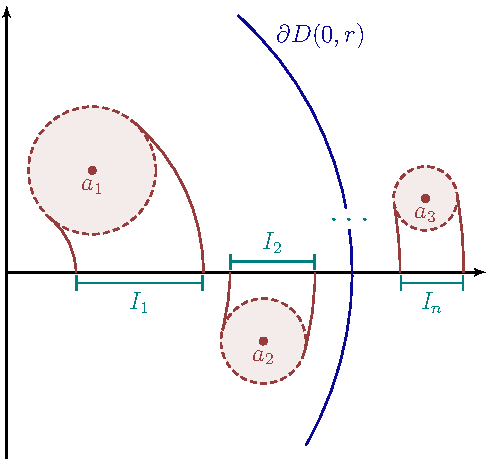
\includegraphics{%
                Figuras/In Hadamard.pdf
            }
        \end{figure}
        %
        Ora, mas a união dos $I_n$ não pode cobrir $[L, L+1]$ já que
        %
        \begin{align*}
            \Leb\left(
            \bigcup_{n=n_0}^{\infty} I_n
            \right) 
            \leq
            \sum_{n=n_0}^{\infty} \Leb(I_n)
            =
            \sum_{n=n_0}^{\infty} \frac{2}{|a_n|^{k+1}}
            <
            \frac{2}{10},
        \end{align*}
        %
        enquanto que $\Leb([L, L+1]) = 1$. Portanto, podemos encontrar 
        a sequência desejada $(r_n)_{n\in\N}$ com $r_n \xrightarrow{n\to\infty} \infty$
        aplicando o Lema \ref{lema:5.3-Stein}.
    \end{proof}
    %
    
    \medskip
    
    Antes de rumar para a demonstração do teorema de Hadamard, vamos precisar de um último
    lema.
    %
    \begin{lema}
    \label{lema:5.5-Stein}
        Seja $g:\C\to\C$ uma função inteira tal que, para algum $s>0$,
        %
        \begin{equation*}
            \Re(g(z)) \leq C r^s
        \end{equation*}
        %
        sempre que $|z| = r$ para uma sequência de números reais positivos $r$ que tende para o infinito.
        Então $g$ é um polinômio de grau menor ou igual a $s$.
    \end{lema}
    %
    \begin{proof}
        Expandindo $g$ em série de potências ao redor da origem, temos
        %
        \begin{equation*}
            g(z) = \sum_{n=0}^{\infty} a_n z^n.
        \end{equation*}
        %
        Observe que $a_k = g^{(k)}(0)/k!$. Usando a fórmula integral de Cauchy e lembrando como as derivadas de $g$ se expressam por meio desta fórmula, temos que, para $n \geq 0$,
        %
        \begin{align*}
            a_n = \frac{g^{(n)}(0)}{n!} &= \frac{1}{2\pi i} \int_{\partial D_r} \frac{g(w)}{(w - 0)^{n+1}} \, dw \\
            &= \frac{1}{2\pi r^n} \int_{0}^{2\pi} g(re^{i\theta})e^{-in\theta} \, d\theta.
        \end{align*}
        %
        A mesma identidade vale para $n < 0$, mas, nesse caso a integral se anula, pois $g(w)/w^{n+1} = g(w)w^{-n-1}$ é holomorfa. Concluímos, então, que
        \begin{equation*}
            \frac{1}{2\pi} \int_0^{2\pi} g(re^{i\theta}) e^{-in\theta} \, d\theta
            =
            \begin{cases}
                a_n r^n, n \geq 0 \\
                0, n < 0
            \end{cases}.
        \end{equation*}
        %
        Tomando conjugados complexos, obtemos
        %
        \begin{equation*}
            \frac{1}{2\pi} \int_0^{2\pi} \overline{ g(re^{i\theta}) } e^{-in\theta} \, d\theta = 0
        \end{equation*}
        %
        sempre que $n > 0$. Como $2\Re(g) = g + \overline{g}$, adicionamos as duas equações
        acima para obter
        %
        \begin{equation*}
            a_n r^n = \frac{1}{\pi} \int_0^{\pi} \Re(g(re^{i\theta}))e^{-in\theta} \, d\theta,
            \, n > 0.
        \end{equation*}
        %
        Para $n = 0$, tomamos a parte real em ambos os lados da primeira integral para encontrar
        %
        \begin{equation*}
            2\Re(a_0) = \frac{1}{\pi}\int_0^{2\pi} \Re(g(re^{i\theta})) \, d\theta.
        \end{equation*}
        %
        Agora, notamos o fato de que para todo $n\neq 0$ a integral de $e^{-in\theta}$
        em qualquer circunferência de centro na origem é nula. Portanto,
        %
        \begin{equation*}
            a_n 
            = 
            \frac{1}{\pi r^n} \int_0^{2\pi} \left[ \Re(g(re^{i\theta})) - Cr^s \right]e^{-in\theta}
            \, d\theta, \, n > 0,
        \end{equation*}
        %
        e segue que
        %
        \begin{equation*}
            |a_n| 
            \leq
            \frac{1}{\pi r^n} 
            \int_0^{2\pi} \left[ Cr^s - \Re(g(re^{i\theta})) \right] \, d\theta
            \leq
            2Cr^{s-n} - 2\Re(a_0)r^{-n}.
        \end{equation*}
        %
        Fazendo $r\to\infty$, obtemos que $a_n = 0$ para $n > s$, de modo que $g$
        é um polinômio de grau no máximo $s$, como desejado.
    \end{proof}
    %
    
    \medskip
    
    Agora, para provar o teorema de Hadamard, seja
    %
    \begin{equation*}
        E(z) = z^m \prod_{n=1}^{\infty} E_k(z/a_n).
    \end{equation*}
    %
    Para mostrar que $E$ é inteira, aplicamos a Proposição \ref{prop:prod-inf-func-holom} notando que
    %
    \begin{equation*}
        |1 - E_k(z/a_n)| \leq c\left| \frac{z}{a_n} \right|^{k+1}
    \end{equation*}
    %
    para todo $n$ suficientemente grande (como no Lema \ref{lema-wstr-est-factor}) e também que
    %
    \begin{equation*}
        \sum_{n=0}^{\infty} \frac{1}{|a_n|^{k+1}}
    \end{equation*}
    %
    converge, pois $\rho_0 < s < k+1$, . Além disso, $E$ tem os mesmos zeros 
    que $f$, de modo que $f/E$ é holomorfa e não se anula em lugar nenhum,
    ou seja,
    %
    \begin{equation*}
        \frac{f(z)}{E(z)} = e^{g(z)}
    \end{equation*}
    %
    para alguma função inteira $g$. Como $f$ tem ordem de crescimento
    $\rho_0$ e pela estimativa para $E$ obtida no Corolário \ref{cor-seq-raios-inf},
    temos
    %
    \begin{align*}
        \exp(\Re(g(z))) &= \left| \frac{f(z)}{E(z)} \right| \\
                        &\leq \frac{A_1 \exp( B_1|z|^{\rho_0} )}{A_2 \exp( -B_2|z|^{s} )} \\
                        &= A_1 \exp(B_1 |z|^{\rho_0} + B_2 |z|^s) \\
                        &\leq A_1 \exp(B_3 |z|^s).
    \end{align*}
    %
    para $|z| = r_m$. Isso mostra que
    %
    \begin{equation*}
        \Re(g(z)) \leq A_2|z|^s, \, |z| = r_m
    \end{equation*}
    %
    e segue do Lema \ref{lema:5.5-Stein} que $g$ é um polinômio de grau menor
    ou igual a $s$, terminando a demonstração.
    %
    % falar do teo de Mittag-Leffler e da aplicação para funções com imagens prescritas (?)
 
 
 
 
 
    \subsection{O Pequeno Teorema de Picard}
    
    Nesta seção vamos mostrar, como consequência do Teorema de Hadamard, um resultado fascinante devido a Picard. Ele afirma, entre outras coisas, 
    que a imagem de uma função inteira, de ordem de crescimento finita, pode omitir no máximo um ponto do plano complexo! 
    Isto é, se $f:\C\to\C$ é uma função inteira com ordem de 
    crescimento $0\leqslant \rho<+\infty$, então a o conjunto imagem $f(\C)$ 
    é todo o plano complexo, exceto por, possivelmente, um ponto.
    Este resultado é conhecido como o {\it Pequeno Teorema de Picard}. Seu enunciado mais preciso é apresentado logo abaixo.
 
    
        %
        \begin{teorema}[Pequeno Teorema de Picard]
        \label{teo:pequeno-picard}
        \index{Pequeno Teorema de Picard}
            Se $f:\C\to\C$ é uma função inteira não constante e com ordem de crescimento 
            $\rho \in [0,+\infty)$, então
            %
            \[
              \sharp (f(\C))^c \leq 1.
            \]
            %
            Além do mais,
            \begin{itemize}
                \item se $0\leqslant \rho<1$, então $f(\C)=\C$; 
                
                \item se $1\leqslant \rho<+\infty$, então 
                a imagem de $f$ omite no máximo um ponto do plano complexo 
                e todo ponto da imagem de $f$ possui infinitas pré-imagens.
            \end{itemize}
        \end{teorema}

        \medskip 
        %
        Antes de apresentar a prova do Teorema de Picard vamos enunciar um pequeno lema preliminar, um corolário do Teorema Fundamental da Álgebra.
        
        \medskip 
        %
        \begin{lema}
        \label{lema-pol-sobrejetor}
            Todo polinômio não constante $P:\C\to\C$ é sobrejetor.
        \end{lema}
        %
        \begin{proof}[Demonstração do lema]
            Dado $w\in\C$, o polinômio $P(z) - w$ é não constante e, pelo
            Teorema Fundamental da Álgebra, tem uma raiz $z_w$. Ora, então
            $P(z_w) = w$ e, portanto, $P$ é sobrejetor.
        \end{proof}
        
        \medskip
        %
        Vamos, então, à demonstração do Pequeno Teorema de Picard.
        %
        \begin{proof}[Demonstração do Pequeno Teorema de Picard]
            Suponha que existe algum $a\in\C$ tal que
            %
            \[
            f(z) - a \neq 0, \quad \forall z\in\C.
            \]
            %
            Em outras palavras, estamos supondo que a função inteira $g:\C\to\C$ 
            dada por $g(z)= f(z)-a$ não possui raízes. 
            Observe que $g$ é uma função inteira de ordem de crescimento 
            finito $\rho$. Portanto, podemos aplicar o Teorema da 
            Fatoração de Hadamard (Teorema \ref{teo:fatoracao-hadamard}) 
            para garantir que 
            %
            \begin{align}
            \label{eq-aux1-litle-picard}
                f(z) - a = e^{P(z)},
            \end{align}
            %
            onde $P(z)$ é um polinômio de grau no máximo $\rho$.
            
            \medskip 
            Vamos separar o restante do argumento em dois casos.
            \begin{itemize}
                \item Caso 1. $0\leqslant \rho<1$;
                \item Caso 2. $1\leq\rho<+\infty$.
            \end{itemize}
            \medskip 
            
            
            Caso 1. Neste caso, como $0\leqslant \rho<1$, então  
            segue do Teorema da Fatoração de Hadamard que
            o polinômio que aparece no lado direito de
            \eqref{eq-aux1-litle-picard} é tal que
            $\textrm{grau}(P)=\lfloor \rho \rfloor =0$, ou seja, 
            $P$ é constante. Mas então existe 
            alguma constante $K\in \C$ tal que 
            $f(z)-a=e^K$ para todo $z\in\C$, o que 
            é um absurdo, pois por hipótese 
            $f$ é não-constante. 
            
            O absurdo vem de termos assumido que existe um número complexo $a$ tal que a função $g=f-a$ não possui raízes. Desta forma, para todo $a\in\C$ fixado, existe algum $z\in \C$ 
            tal que $f(z)=a$ e, portanto, $f(\C)=\C$.
            
            
            \bigskip
            Caso 2.
            Neste segundo caso, sabemos que $P$ tem grau no máximo
            $\rho \geq 1$. Se, por ventura, $P$ for constante,
            então voltamos ao caso anterior.
            
            Assumamos então $P$ não constante.
            Já que todo ponto não-nulo do plano complexo
            pode ser representado em coordenadas polares, podemos afirmar que dado um ponto arbitrário 
            $b\in \C\setminus\{a\}$,
            existe algum $\varphi \in [0, 2\pi)$ tal que
            %
            \[
            b - a = |b - a| e^{i\varphi}.
            \]
            %
            Usando o Lema \ref{lema-pol-sobrejetor},
            podemos garantir que existe um número complexo $z_b\in\C$ tal que
            %
            \begin{align*}
                P(z_b) = \ln|b-a| + i\varphi.
            \end{align*}
            %
            Substituindo $z$ por $z_b$ em
            \eqref{eq-aux1-litle-picard} e usando a igualdade acima ficamos com
            %
            \[
            f(z_b) - a = b - a 
            \qquad \iff \qquad f(z_b) = b.
            \] 
            %
            Consequentemente, a  
            imagem do $f$ pode omitir 
            no máximo um ponto de $\C$.
            
            Para mostrar que a imagem inversa de qualquer ponto 
            $b\in \C\setminus\{a\}$ possui infinitos pontos, basta 
            observar que para cada $k\in\Z$, podemos usar 
            novamente o Lema \ref{lema-pol-sobrejetor}
            para garantir que existe um ponto 
            $z_{b,k}\in \C$
            tal que 
            \begin{align*}
                P(z_{b,k}) = \ln|b-a| + i(\varphi+2k\pi).
            \end{align*}
            Argumentando de maneira análoga, 
            concluímos que 
            $f(z_{b,k})=b$. 
            Já que para qualquer par de inteiros distintos $k$ e $k'$
            temos $z_{b,k}\neq z_{b,k'}$, pois 
            $\Im(P(z_{b,k}))\neq \Im(P(z_{b,k'}))$, 
            segue que $b$ tem infinitas pré-imagens. 
            Como $b\in \C\setminus\{a\}$
            é arbitrário, finalizamos a prova do teorema.
        \end{proof}
        %
        
        
        
\section{A função Gama}

    O fatorial é uma aplicação conhecida de todos que, para cada inteiro não negativo $n$ 
    associa $n! \equiv n \cdot (n-1) \cdots 3 \cdot 2 \cdot 1$ e convenciona-se $0! = 1$. 
    Podemos expressar os fatoriais como integrais reais por meio da identidade
    %
    \[ 
    (n-1)! = \int_0^{\infty}e^{-t} t^{n-1} \, dt.
    \]
    %
    Nesta seção, vamos estudar a função Gama, que será denotada por $\Gamma$. Ela é uma função de grande importância na Análise 
    Matemática e na Teoria Analítica dos Números. 
    Esta função pode ser vista como uma extensão 
    do conceito de fatorial de um número natural. 
    Para cada $s>0$, definimos
    %
    \begin{align}
        \label{def-func-gamma-real}
    \Gamma(s) \equiv \int_0^{\infty}e^{-t} t^{s-1} \, dt.
    \end{align}
    %
    Primeiro, vamos mostrar que $\Gamma$ está bem definida. Problemas de convergência 
    podem ocorrer quando $t = 0$ e $s - 1 < 0$ e também conforme $t$ toma valores muito grandes.
    
    Observe que $s - 1 < 0$ ocorre somente se $0 < s < 1$. Vamos mostrar que a integral 
    de 0 a 1 é limitada. Seja $\e > 0$ qualquer, então
    %
    \begin{align*}
        \left| \int_{\e}^{1}e^{-t}t^{s-1} \, dt \right| 
        &\leq \int_{\e}^{1}t^{s-1} \, dt \\[0.3cm]
        &= \frac{t^s}{s}\Big |_{\e}^{1} \\[0.3cm]
        &= \frac{1}{s} - \frac{\e^s}{s} \xrightarrow{\ \e\to 0\ } \frac{1}{s}.
    \end{align*}
    %
    Esta simples estimativa mostra a razão de escolhermos $s > 0$. 
    No entanto, isto não mostra completamente o por quê desta escolha.
    O segundo motivo é que, se $s = -\delta < 0$, então
    %
    \begin{align*}
        \int_{\e}^{1}e^{-t}t^{s-1} \, dt &= \int_{\e}^{1}e^{-t}t^{-1-\delta} \, dt \\[0.3cm]
        &\geq \int_{\e}^{1}t^{-1-\delta} \, dt \\[0.3cm]
        &= \frac{t^{-\delta}}{\delta}\Big |_{t = \e}^{1} \\[0.3cm]
        &= \frac{\e^{-\delta}}{\delta} - \frac{1}{\delta} \xrightarrow{\ \e\to 0\ } \infty.
    \end{align*}
    %
    
   
    
    Analisamos agora a outra porção da integral. Primeiro, observe que $e^{-t/2}t^{s-1}$ 
    vai a 0 conforme $t$ cresce. Isto mostra que esta expressão é limitada. Então
    %
    \begin{align*}
        \int_{1}^{1/\e}e^{-t}t^{s-1} \, dt &\leq M\int_{\e}^{1}e^{-t/2} \, dt \\[0.3cm]
        &= 2M(e^{-1/2} - e^{-1/2\e}) < \infty
    \end{align*}
    %
    para todo $\e > 0$. 
    Estas considerações mostram que a função $\Gamma$ está bem 
    definida para todo $s > 0$.
    
    O nosso objetivo é estender $\Gamma$ para todo o plano complexo. 
    Tentaremos realizar tal extensão admitindo que $s$ seja um número complexo. 
    Inicialmente, consideraremos o semiplano $\Re(s) > 0$.
    
    
    \begin{lema}
    \label{lema-conv-abs-cond-int-imp}
        Sejam $\Omega \subseteq \C$ um domínio e 
        $f: \Omega \times (0,\infty)\to \C$ uma função. 
        Assuma que para cada $z \in \Omega$ fixado, 
        que o conjunto de descontinuidades da função 
        $t \mapsto f(z,t)$ tenha medida de Lebesgue nula. 
        Além disso, assuma que para $z\in \Omega$ fixado e cada $\delta>0$ dado que 
        %
        \[
        \sup_{t \in [\delta,1/\delta]} |f(z,t)| < \infty.
        \]
        %
        Se $z\in \Omega$ fixado é tal que o seguinte limite existe
        %
        \[
        \lim_{\delta \to 0} 
        \int_{\delta}^{ \frac{1}{\delta} }
        |f(z,t)| \, dt
        \equiv 
        \int_{0}^{\infty} |f(z,t)|\, dt ,
        \]
        %
        então para cada $z\in\Omega$, existe o limite 
        %
        \[
        g(z) \equiv \lim_{\delta \to \infty} 
        \int_{\delta}^{ \frac{1}{\delta} }f(z,t) \, dt
        \equiv
        \int_{0}^{\infty }f(z,t) \, dt.
        \]
        %
    \end{lema}
    %
    \begin{proof}
        Fixado $z\in \Omega$ e dado $\delta>0$ temos diretamente
        das hipóteses do lema que a integral abaixo existe e é finita
        %
        \[
        \int_{\delta}^{ \frac{1}{\delta}  }|f(z,t)| \, dt.
        \]
        %
        Além disso, por hipótese temos garantia da existência do seguinte
        limite:
        %
        \[
        I \equiv \lim_{\delta \to \infty} 
        \int_{\delta}^{ \frac{1}{\delta} }|f(z,t)| \, dt.
        \]
        % 
        Isto significa que, dado $\e > 0$ qualquer, existe 
        $\delta_0\equiv \delta_0(\varepsilon,z) > 0$ tal que, para todo
        $0<\delta < \delta_0$  temos
        %
        \[
        \Big | I - \int_{\delta}^{ \frac{1}{\delta} }|f(z,t)| \, dt \Big | < \e.
        \]
        %
        Usando a desigualdade triangular 
        podemos verificar que para quaisquer par de
        números reais $\rho$ e $\delta$ satisfazendo
        $0<\rho,\, \delta <\delta_0$, temos
        %
        \begin{align}
        \label{eq-aux1-lema-conv-abs-cond-int-imp}
        \left| 
            \int_{\rho}^{ \frac{1}{\rho} }|f(z,t)| \, dt
            -
            \int_{\delta}^{ \frac{1}{\delta} }|f(z,t)| \, dt
        \right| 
        &= 
        \left| 
            \int_{\rho}^{ \frac{1}{\rho} }|f(z,t)| \, dt - I
            +
            I -\int_{\delta}^{ \frac{1}{\delta} }|f(z,t)| \, dt
        \right|
        \nonumber\\[0.3cm]
        &\leqslant
        \left| 
            I- \int_{\rho}^{ \frac{1}{\rho} }|f(z,t)| \, dt 
        \right|
        +
        \left| 
            I -\int_{\delta}^{ \frac{1}{\delta} }|f(z,t)| \, dt
        \right|
        \nonumber\\[0.3cm]
        &<
        2\e.
        \end{align}
        %
        Seja $(a_n)_{n\in\N}$ uma sequência arbitraria de números reais estritamente positivos tal que 
        $a_n\to 0$, quando $n\to\infty$ e defina para cada $n\in\N$
        %
        \[
        I_n  
        \equiv 
        I_n(z) 
        \equiv
        \int_{ a_n }^{ \frac{1}{a_n} }f(z,t) \, dt.
        \]
        %
        Como $(a_n)_{n\in \N}$ é uma sequência arbitrária
        tudo que precisamos para finalizar a prova do lema é mostrar que a sequência $(I_n)_{n\in\N}$ é uma sequência de Cauchy e, em seguida,
        mostrar que o limite desta sequência é independente da escolha
        particular de $(a_n)_{n\in \N}$. 
        
        Já que $a_n\to 0$, quando $n\to\infty$, sabemos que dado 
        $\e>0$, existe $n_0\in\N$ tal que para todo $n,m\geqslant n_0$
        temos $0< a_n,\, a_m <\delta_0$. Portanto segue diretamente da desigualdade \eqref{eq-aux1-lema-conv-abs-cond-int-imp}
        que 
        \begin{align*}
            |I_n - I_m| 
            = 
            \left| 
            \int_{a_n}^{ \frac{1}{a_n} }f(z,t) \, dt 
            - \int_{ a_{m} }^{ \frac{1}{a_m} }f(z,t) \, dt 
            \right|
            <2\e.
        \end{align*}
        %
        O que mostra que $(I_n)_{n\in\N}$ é uma sequência de Cauchy
        e consequentemente uma sequência convergente. 
        Denote por $J$ o limite desta sequência. 
        A rigor, observamos que o valor deste limite poderia depender 
        da particular escolha da sequência $(a_n)_{n\in\N}$. 
        Mas aqui este não é o caso e para suportar esta afirmação  
        vamos mostrar que este limite é o 
        mesmo para qualquer sequência de número reais positivos 
        que converge para zero. 
        
        Suponha que $J_1, J_2$ são limites obtidos usando 
        duas sequências distintas de números reais positivos que convergem para zero, digamos $(a_n)_{n\in\N}$ e $(b_n)_{n\in\N}$,
        respectivamente. 
        
        Nestas condições, dado $\e>0$ podemos encontrar $n_0\in\N$ tal 
        que para todo $n\geqslant n_0$ temos
        $0<a_n,\ b_n <\delta_0$ e também
        \[
        \left|J_1-\int_{a_n}^{ \frac{1}{a_n} }f(z,t) \, dt \right|<\e
        \qquad\text{e}\qquad
        \left|J_2-\int_{b_n}^{ \frac{1}{b_n} }f(z,t) \, dt \right|<\e.
        \]
        
        Usando a desigualdade triangular, 
        as três últimas desigualdades acima e em seguida a desigualdade \eqref{eq-aux1-lema-conv-abs-cond-int-imp}
        podemos concluir que 
        %
        \begin{align*}
            |J_1& - J_2| 
            \\[0.3cm]
            &= 
            \left| 
            J_1-\int_{a_n}^{ \frac{1}{a_n} }f(z,t) \, dt 
            +\int_{a_n}^{ \frac{1}{a_n} }f(z,t) \, dt 
            - \int_{ b_{n} }^{ \frac{1}{b_n} }f(z,t) \, dt
            +
             \int_{ b_{n} }^{ \frac{1}{b_n} }f(z,t) \, dt
             -J_2
            \right| 
            \\[0.3cm]
            &\leqslant
            \left| 
            J_1-\int_{a_n}^{ \frac{1}{a_n} }\!\! f(z,t) \, dt 
            \right|
            +
            \left|
            \int_{a_n}^{ \frac{1}{a_n} }\!\! f(z,t) \, dt 
            - \int_{ b_{n} }^{ \frac{1}{b_n} }\!\! f(z,t) \, dt
            \right|
            +
            \left|
             \int_{ b_{n} }^{ \frac{1}{b_n} }\!\!\! f(z,t) \, dt
             -J_2
            \right|
            \\[0.3cm]
            &<4\e.
        \end{align*}
        %
       Como $\e>0$ na desigualdade acima é arbitrário, 
       temos obrigatoriamente $J_1=J_2$. 
       Com isto encerramos a prova do lema.
    \end{proof}
    %
    \begin{observacao}
        No lema anterior, assumimos que a função $f$ com $z$ fixado tem um conjunto de descontinuidades com medida de Lesbegue nula, isto é equivalente a dizer que ela é Riemann integrável 
        em relação à variável $t$ real. Além disso, vale um resultado análogo ao anterior: Se assumimos que existe 
        %
        \[
        \lim_{a \to \infty} \int_{-a}^{a}|f(z,t)| \, dt,
        \]
        %
        então podemos mostrar similarmente que existe
        %
        \[
        \lim_{a \to \infty} \int_{-a}^{a}f(z,t) \, dt.
        \]
        %
    \end{observacao}
    
    
    \bigskip 
    
    
    Seja $s \in \C$ e denote $\sigma = \Re(s)$. Então 
    para todo $t>0$ temos que 
    %
    \begin{align*}
        |t^{s-1}| &= |\exp((s-1)\ln t)| \\
        %
        &= \exp(-\ln{t})|\exp(s\ln t)| \\
        %
        &= \exp(-\ln{t})|\exp(\sigma\ln t)| \\
        %
        &= t^{\sigma - 1}.
    \end{align*}
    %
    Além do mais, para qualquer $\delta>0$ dado,
    temos as seguinte estimativa
    \[
    \sup_{t\in [\delta,1/\delta]} |e^{-t}t^{s-1}|
    =
    \sup_{t\in [\delta,1/\delta]} e^{-t}t^{\sigma-1}
    <+\infty.
    \]
    %
    Tomando $\sigma=\Re(s)>0$ temos também que 
    \begin{equation*}
        \int_{0}^{\infty}|e^{-t}t^{s-1}| \, dt = \int_{0}^{\infty}e^{-t}|t^{s-1}| \, dt = \int_{0}^{\infty}e^{-t}t^{\sigma-1} \, dt 
        = 
        \Gamma(\sigma)<+\infty,
    \end{equation*}
    %
    Seja $\Omega\equiv \{s\in\C: \Re(s)>0\}$. 
    Já que a aplicação $f:\Omega\times (0,\infty)\to\C$ dada por 
    $f(s,t)= e^{-t}t^{s-1}$ é contínua, segue 
    das observações acima que podemos aplicar o lema anterior para 
    provar que existe
    %
    \[
    \Gamma(s)\equiv \int_{0}^{\infty}e^{-t}t^{s-1} \, dt,
    \]
    para todo $s\in\C$ tal que $\Re(s)>0$. 
    %
    \begin{teorema}
        A função $\Gamma:(0,\infty)\to\R$ definida em \eqref{def-func-gamma-real}
        admite uma extensão analítica para o semiplano 
        $\{s \in \C : \Re(s) >0 \}$ e além do mais para qualquer ponto
        $s$ neste semi-plano esta extensão analítica é representada pela
        seguinte integral 
        \[
        \Gamma(s)\equiv \int_{0}^{\infty}e^{-t}t^{s-1} \, dt
        \]
    \end{teorema}
    %
    \begin{proof}
        Naturalmente, a função que é candidata a ser a extensão de $\Gamma(s)$ 
        é aquela que tem a mesma expressão, mas em que admitimos que a variável $s$ seja complexa.
        Aqui, por abuso de linguagem, denotaremos esta candidata por $\Gamma(s)$ também. Sejam 
        $
        0 < \delta < M$ quaisquer números reais positivos fixados e 
        considere a faixa $S\equiv  S_{\delta, M} 
        \equiv 
        \{ s \in \C : \delta < \Re(s) < M\}$. 
        Vamos mostrar, para quaisquer escolhas das constantes $\delta$ e $M$, que a função $s\longmapsto\Gamma(s)$ definida na faixa $S$ é o limite uniforme da sequência de funções $(g_n)_{n\in \N}$, onde
        %
        \[
        g_n(s) = \int_{1/n}^{n}e^{-t}t^{s-1} \, dt.
        \]
        %
        Vamos mostrar também que $g_n$ é uma função holomorfa,
        para cada $n\in \N$ e concluir então que $\Gamma$ é holomorfa na faixa $S$. 
        
        Para provar as afirmações feitas acima, vamos começar mostrando que para cada $n\in \N$ fixado que $g_n:S\to C$ é uma função contínua. De fato, seja $s_0 \in S$ temos  
        %
        \begin{align*}
            |g_n(s)-g_n(s_0)|
            &=
            \left|
            \int_{1/n}^{n}e^{-t}t^{s-1} \, dt
            -
            \int_{1/n}^{n}e^{-t}t^{s_0-1} \, dt
            \right|
            \\[0.3cm]
            &\leqslant
            \int_{1/n}^{n} |t^{s-1}-t^{s_0-1}| \, dt
            \\[0.3cm]
            &\leqslant
            \int_{1/n}^{n}
            \frac{1}{t} |t^{s}-t^{s_0}|            
            \, dt
            \\[0.3cm]
            &\leqslant
            n
            \int_{1/n}^{n}
            |t^s-t^{s_0}| \, dt.
        \end{align*}
        %
    
    Observe agora que a aplicação $s \mapsto t^s = \exp(s\ln t)$ é contínua e $ I_n = [1/n, n]$ é compacto, então podemos encontrar $\delta > 0$ tal que $\sup_{t \in I_n} |t^s-t^{s_0}| < \e/n^2$ quando $|s - s_0| < \delta$. Para verificar isto note que, fixado $t \in I_n$ e dado $\e/n^2 > 0$, encontramos $\delta_t > 0$ tal que $|t^s - t^{s_0}| < \e/n^2$ sempre que $|s - s_0| < \delta_t$. Como $t \mapsto t^s$ também é contínua, há uma vizinhança $B_t = (t-\xi_t, t+ \xi_t)$ de $t$ em que ainda vale a mesma estimativa. As bolas $B_t$ formam uma cobertura de $I_n$ por abertos, então, por compacidade, há uma subcobertura finita com centros $t_1, t_2, \dots, t_r$. Seja $\delta = \min\{\delta_{t_1}, \dots, \delta_{t_r}\}$, então $|s - s_0| < \delta$ implica que $|t^s-t^{s_0}| < \e/n^2$ para todo $t \in I_n$, ou seja, $\sup_{t \in I_n} |t^s-t^{s_0}| < \e/n^2$. 
    
    Com esta estimativa, temos 
    %
    \begin{align*}
        |g_n(s)-g_n(s_0)| &\leq n
            \int_{1/n}^{n}
            |t^s-t^{s_0}| \, dt\\
            %
            &\leq n \frac{\e}{n^2}\int_{1/n}^{n} \, dt \\
            %
            &= n\left(n-\frac{1}{n}\right)\frac{\e}{n^2} \\
            %
            &\leq \e.
    \end{align*}
    %
    Isto mostra que as $g_n$ são funções contínuas.
        
    Próximo passo é mostrar que a integral de $g_n$ ao longo de qualquer
    triângulo contido em $S$ é nula. 
    Para isto, seja $\Delta$ um triângulo arbitrário, contido em $S$. 
    Como a função no integrando que define $g_n$ é contínua, 
    segue do Teorema de Fubini que
        %
        \begin{align*}
            \int_{\Delta}g_n(s)\, ds &= \int_{\Delta}\int_{1/n}^{n}e^{-t}t^{s-1} \, dt \, ds \\
            &= \int_{1/n}^{n} \int_{\Delta} e^{-t}t^{s-1} \, ds \, dt  \\
            &= \int_{1/n}^{n} 0 \, dt = 0.
        \end{align*}
        %
        Já que $\Delta$ é um triângulo qualquer em $S$ e $g_n$ é contínua segue finalmente do Teorema de Morera que $g_n$ é holomorfa.
        
        
        
    \bigskip 
    
    Vamos mostrar agora que $g_n$ converge uniformemente,
    quando $n\to\infty$, para $\Gamma$. De fato, dado qualquer
    $s\in S$ temos 
        %
        \begin{align*}
            |\Gamma(s) - g_n(s)| &= \Big | \int_{0}^{\infty}e^{-t}t^{s-1} \, dt -  \int_{1/n}^{n}e^{-t}t^{s-1} \, dt \Big | \\
            %
            & = \Big | \int_{0}^{1/n}e^{-t}t^{s-1} \, dt +  \int_{n}^{\infty}e^{-t}t^{s-1} \, dt \Big | \\
            %
            &\leq \Big | \int_{0}^{1/n}e^{-t}t^{s-1} \, dt \Big | +  \Big | \int_{n}^{\infty}e^{-t}t^{s-1} \, dt \Big | \\
            %
            &\leq \int_{0}^{1/n}e^{-t}|t^{s-1}| \, dt  + \int_{n}^{\infty}e^{-t}|t^{s-1}| \, dt \\
            %
            &\leq \int_{0}^{1/n}t^{\sigma-1} \, dt + \int_{n}^{\infty}e^{-t}t^{\sigma-1} \, dt \\
            %
            &\leq \int_{0}^{1/n}t^{\delta-1} \, dt + \int_{n}^{\infty}e^{-t}t^{M-1} \, dt \\
            %
            &\leq \frac{1}{\delta}\frac{1}{n^\delta} + K_M\int_{n}^{\infty}e^{-t/2} \, dt.
        \end{align*}
        %
        Já que o lado direito da estimativa acima vai a zero,
        quando $n\to\infty$, independentemente da escolha de $s\in S$, segue que $\Gamma(s)$ é holomorfa na faixa 
        $S$ \textcolor{red}{(citar teorema)}. 
        Lembrando que as constantes $M$ e $\delta$ são arbitrárias, 
        podemos concluir que $\Gamma(s)$ é holomorfa em todo $U$.
    \end{proof}
    
    
    \bigskip 
    
    A seguir, mostramos que a função Gama satisfaz uma equação funcional.
    Esta equação funcional será usada para revelar diversas propriedades 
    da função Gama, que não são simples de serem obtidas à partir 
    de sua definição.
    Vamos usá-la para dar uma prova de que função Gama pode ser estendida à 
    função meromorfa em $\C$ bem como para determinar os resíduos 
    de Gama em cada uma de suas singularidades.  
    %
    
    
    Apesar de toda sua aplicabilidade e incríveis consequências a equação funcional pode ser obtida por uma simples aplicação do método de integração por partes, como mostramos a seguir. 
    
    Pela regra do produto, temos que
    %
    $$\frac{d}{dt}(e^{-t}t^{s}) = se^{-t}t^{s-1} - e^{-t}t^{s}.$$
    %
    Considerando que $s$ satisfaz $\Re(s)>0$, integrando ambos os lados da igualdade acima e usando o Teorema Fundamental do Cálculo obtemos
    %
    \begin{align*}
        0 
        &= 
        \lim_{\e \to 0^+} e^{-t}t^s \Big|_{\e}^{1/\e} 
        \\[0.3cm]
        %
        &= 
        \lim_{\e \to 0^+} s\int_{\e}^{1/\e} e^{-t}t^{s-1} \, dt - \int_{\e}^{1/\e} e^{-t}t^{s} \, dt 
        \\[0.3cm]
        %
        &= 
        s\Gamma(s) - \Gamma(s+1).
    \end{align*}
    %
    Portanto, fica demonstrado o seguinte teorema.
    
    \begin{teorema}\label{teo-eq-func-Gama}
    Se $\Re(s)>0$, então $\Gamma(s+1) = s\Gamma(s)$.
    \end{teorema}

    Note que podemos concluir do teorema 
    acima a validade da afirmação feita 
    no início desta seção, isto é, 
    $\Gamma(n) = (n-1)!$, 
    para todo $n > 0$ inteiro. 
    
    \begin{teorema}
    \label{teo-cont-meromorfa-gamma}
        A função $\Gamma$, inicialmente definida para $\Re(s) > 0$, admite uma continuação analítica à uma função meromorfa em $\C$ com polos simples nos inteiros não positivos. Além disso, o resíduo em $-n$ é $(-1)^{n}/n!$ para todo $n \in \N \cup \{0\}$.
    \end{teorema}
    \begin{proof}
    Para cada $m \in \N$, defina 
    \[
    U_m = \{s \in \C \setminus \{0,-1, \dots, -(m-1)\}: \Re(s) > -m \}.
    \]
    Vamos definir a continuação de $\Gamma$ por etapas, primeiro a estendemos para $U_1$, depois para $U_2$ e assim sucessivamente. Seja $F_1 : U_1 \to \C$ dada por
    %
    $$F_1(s) = \frac{\Gamma(s+1)}{s}.$$
    %
    Quando $\Re(s) > 0$, podemos concluir da equação funcional de $\Gamma$ que 
    %
    $$F_1(s) = \frac{s\Gamma(s)}{s} = \Gamma(s),$$
    %
    logo, $F_1$ e $\Gamma$ coincidem neste semiplano. Em particular, $F_1$ é holomorfa porque é definida a partir de $\Gamma$ e, quando $\Re(s)> -1$, temos $\Re(s+1) > 0$. Observe ainda que
    %
    $$ \lim_{s \to 0} sF_1(s) = \Gamma(1) = 1 \neq 0,$$
    %
    então $s=0$ é um polo simples de $F_1$ com resíduo neste ponto sendo igual à $1$.
    
    Definimos agora a função holomorfa $F_2 : U_2 \to \C$ 
    pela seguinte expressão
    %
    $$F_2(s) = \frac{\Gamma(s+2)}{s(s+1)}.$$
    %
    Quando $\Re(s) > -1$, podemos usar a equação funcional e observar que $F_2(s) = F_1(s)$ neste semiplano. Além disso, 
    %
    $$ \lim_{s \to -1} (s+1)F_2(s) = \lim_{s \to -1} \frac{\Gamma(s+2)}{s} = \frac{\Gamma(1)}{-1} = -1 \neq 0$$
    %
    e temos $\res(F_2,-1) = -1$. 
    
    Continuamos deste modo definindo $F_{n+1} : U_{n+1} \to \C$ por
    %
    $$F_{n+1}(s) = \frac{\Gamma(s+n+1)}{(s+n)(s+n-1) \cdots (s+1)s}.$$
    %
    Como anteriormente, esta função também é holomorfa e temos
    %
    \begin{align*}
        \lim_{s \to -n} (s+n)F_{n+1}(s) &= \lim_{s \to -n} (s+n)\frac{\Gamma(s+n+1)}{(s+n)(s+n-1) \cdots (s+1)s} \\
        &= \frac{\Gamma(1)}{(-1)(-2) \cdots [-(n-1)](-n)} = \frac{(-1)^n}{n!}
    \end{align*}
    %
    mostrando que $F_{n+1}$ tem um polo simples em $s=-n$ e que o resíduo desta função neste polo é exatamente $(-1)^n/n!$. 
    
    Usando os fatos demonstrados acima podemos definir a função $\Gamma$ em todo conjunto $\C\setminus \{0,-1,-2,-3,\ldots\}$
    da seguinte forma. 
    Dado $s\in \C\setminus \{0,-1,-2,-3,\ldots\}$ seja $n\in \N$
    o menor natural tal que $s\in U_n$ e defina $\Gamma(s) \equiv F_n(s)$. Observe que Gama definida assim é uma função bem definida e além do mais todas suas singularidades, 
    isto é, os pontos do conjunto $\{0,-1,-2,-3,\ldots$ são pontos isolados e todos são também polos simples de $\Gamma$ com resíduos dados por 
    \[
    \mathrm{res}(\Gamma,-n) = \frac{(-1)^n}{n!}.
    \]
    \end{proof}
    
    
    
    \begin{corolario}
    \label{cor-eq-func-Gamma}
    Para todo $s\in \C\setminus\{0,-1,-2,-3,\ldots\}$ temos 
    \[
    \Gamma(s+1) = s\Gamma(s).
    \]
    \end{corolario}
    \begin{proof}
    Observe que pelo Teorema \ref{teo-cont-meromorfa-gamma} 
    podemos assegurar que a aplicação 
    \[
    s\longmapsto f(s) = \Gamma(s+1) - s\Gamma(s)
    \] 
    define uma função holomorfa em $\C \setminus \{0, -1, -2, \dots\}$. Pelo Teorema \ref{teo-eq-func-Gama} 
    segue que $f$ é identicamente nula em $\Re(s)> 0$. 
    Já que $\C \setminus \{0, -1, -2, \dots\}$ é um domínio segue do principio da identicamente que $f$ é identicamente nula.
    \end{proof}
    
    \medskip 
    Esta equação funcional é bem conhecida para a função $\Gamma$ real. Então poderíamos usar este fato e ter procedido como fizemos acima para mostrar que ela vale se estende 
    $\Re(s)> 0$. Bastaria definir $f(s)$ para $\Re(s)> 0$ e usar que ela é nula sobre os reais positivos.
    
    Podemos obter a continuação da função $\Gamma$ de uma forma alternativa analisando as integrais parciais
    %
    \begin{equation}
    \label{eq-Gamma1}
    \int_{0}^{1}e^{-t}t^{s-1} \, dt + \int_{1}^{\infty}e^{-t}t^{s-1} \, dt.
    \end{equation}
    %
    Vamos mostrar que a integral à direita define uma função inteira. Defina, para cada $n \in \N$,
    %
    \[
    g_n(s) = \int_{1}^{n}e^{-t}t^{s-1} \, dt
    \]
    %
    para $s \in \C$. Vamos usar o Teorema de Morera para mostrar que cada $g_n$ é holomorfa e vamos verificar que a sequência definida por estas funções converge uniformemente para a integral à direita em (\ref{eq-Gamma1}). Observe que esta integral existe, pois seu módulo é limitado por 
    %
    $$\int_{1}^{\infty}e^{-t}t^{\Re(s) - 1} \, dt < \infty. $$
    
    Sejam $s_0$ um número fixado, então
    %
    \begin{align*}
        |g_n(s) - g_n(s_0)| &= \Big | \int_{1}^{n}e^{-t}(t^{s-1}-t^{s_0-1}) \, dt\Big | \\
        %
        &\leq \int_{1}^{n}\frac{e^{-t}}{t}|t^{s}-t^{s_0}| \, dt \\
        %
        &\leq \int_{1}^{n}|t^{s}-t^{s_0}| \, dt 
    \end{align*}
    %
    Observe que a função $s \mapsto t^s = \exp(s\ln t)$ é inteira e $J_n = [1,n]$ é compacto, então, dado $\e > 0$, podemos encontrar $\delta > 0$ tal que $\sup_{t \in J_n}|t^{s}-t^{s_0}| < \e$ se $|s-s_0| < \delta$. Analogamente ao que fizemos antes, temos 
    %
    \begin{align*}
    |g_n(s) - g_n(s_0)| &\leq \int_{1}^{n}|t^{s}-t^{s_0}| \, dt \\
    %
    &\leq \e \int_{1}^{n} \, dt = (n-1)\e \xrightarrow{\e \to 0} 0.
    \end{align*}
    %
    Isto mostra que as funções $g_n$ são contínuas em $\C$. Se $\Delta$ é um triângulo qualquer
    %
    \begin{align*}
        \int_\Delta g_n(s) \, ds &= \int_\Delta\int_{1}^{n}e^{-t}t^{s-1} \, dt \, ds \\
        %
        &= \int_{1}^{n}\int_\Delta e^{-t}t^{s-1} \, ds \, dt = 0.
    \end{align*}
    %
    Pelo Teorema de Morera, as $g_n$ são holomorfas. Na verdade, não é difícil ver que definem funções inteiras. 
    
    Seja $\sigma = \Re(s)$. Observe que 
    %
    \begin{align*}
        \Big | \int_{1}^{\infty}e^{-t}t^{s-1} \, dt - g_n(s) \Big | &= \Big | \int_{1}^{\infty}e^{-t}t^{s-1} \, dt - \int_{1}^{n}e^{-t}t^{s-1} \, dt \Big | \\
        %
        &= \Big | \int_{n}^{\infty}e^{-t}t^{s-1} \, dt \Big | \\
        %
        &\leq \int_{n}^{\infty}e^{-t}|t^{s-1}| \, dt \\
        %
        &= \int_{n}^{\infty}e^{-t}t^{\sigma-1} \, dt.\\
        %
        &= \int_{n}^{\infty}e^{-t/2}(e^{-t/2}t^{\sigma-1}) \, dt
    \end{align*}
    %
    Devemos mostrar que esta expressão vai a zero quando $n \to \infty$. Para ver isto, analisamos a integral a partir da expressão na ultima desigualdade acima. A função $u(t) = e^{-t/2}t^{\sigma-1}$ definida para $t > 0$ é contínua e tal que $\lim_{t \to \infty} u(t) = 0$, então é limitada superiormente por alguma constante positiva. Usando cálculo em uma variável real, determinamos o máximo desta função, que é $M = e^{-(\sigma -1)}(2(\sigma -1))^{\sigma-1}$ atingido em $t = 2(\sigma-1)$ se $\sigma > 1$. Caso $\sigma < 1$ a função assume valores menores, ainda, pois $0 < t^{\sigma-1} \leq 1$ neste caso. Segue que
    
    \begin{align*}
        \Big | \int_{1}^{\infty}e^{-t}t^{s-1} \, dt - \int_{1}^{n}e^{-t}t^{s-1} \, dt \Big | &\leq M \int_{n}^{\infty}e^{-t/2} \, dt.\\
        %
        &= -2M e^{-t/2} \Big |_{n}^{\infty} \\
        %
        &= 2M e^{-n/2} \xrightarrow{n \to \infty} 0
    \end{align*}
    
    Portanto,
    %
    \[
    \int_{1}^{\infty}e^{-t}t^{s-1} \, dt
    \]
    %
    define uma função inteira, pois é limite uniforme de uma sequência de funções inteiras.
    
    Vamos analisar agora 
    %
    \[
    \int_{0}^{1}e^{-t}t^{s-1} \, dt.
    \]
    %
    Para tanto, vamos considerar a expansão de $e^{-t}$ em série de Taylor. 
    %
    \begin{align}
    \label{Gamma-ext-2}
        \int_{0}^{1}e^{-t}t^{s-1} \, dt &=  \int_{0}^{1}\sum_{n=0}^{\infty}\frac{(-t)^n}{n!} t^{s-1} \, dt \\
        %
        &= \sum_{n=0}^{\infty} \frac{(-1)^n}{n!}\int_{0}^{1}t^{n + s-1} \, dt \\
        %
        &= \sum_{n=0}^{\infty} \frac{(-1)^n}{n!}\frac{t^{n + s}}{s+n} \Big |_{0}^{1} \\
        %
        &= \sum_{n=0}^{\infty} \frac{(-1)^n}{n!(s+n)}.
    \end{align}
    %
    A troca da soma com a integral na segunda igualdade é justificada pelo Lema abaixo.
    %
    \begin{lema}
    \textcolor{red}{Lema para troca integral com soma}
    \end{lema}
    %
    Vamos mostrar que a função em (\ref{Gamma-ext-2}) define uma função meromorfa em $\C$ com polos $0,-1,-2,\dots$. Seja $R>0$ fixado e $N$ um inteiro positivo satisfazendo $N>R>-N+1$. Podemos escrever
    %
    $$ \sum_{n=0}^{\infty} \frac{(-1)^n}{n!(s+n)} = \sum_{n=0}^{N} \frac{(-1)^n}{n!(s+n)} + \sum_{n=N+1}^{\infty} \frac{(-1)^n}{n!(s+n)} = f_N(s) + g(s).$$
    %
    A função $f_N(s)$ é meromorfa no disco $D(0,R)$ e tem polos $0,-1,-2,\dots,-N+1$. De fato, seja $k$ inteiro com $0 \geq k \geq -N+1$, então
    %
    $$\lim_{s \to k} (s+k)f_N(s) = \lim_{s \to k} (s+k)\sum_{n=0}^{N} \frac{(-1)^n}{n!(s+n)} = \lim_{s \to k} (s+k)\frac{(-1)^k}{k!(s+k)} = \frac{(-1)^k}{k!}.$$
    %
    Agora a função $g(s)$ é holomorfa no disco $D(0,R)$. Note que, com $n > N$ e $s \in D(0,R)$, temos $|s+n| \geq N-R+1 > 1$, então
    $1/|s+n| \leq 1/(N-R+1)$. Portanto, cada parcela da soma que define $g(s)$ satisfaz
    %
    $$\frac{(-1)^n}{n!(s+n)} \leq \frac{1}{(N-R+1)n!} = M_n.$$
    %
    Observe que $M_n$ define uma sequência somável. Segue do teste $M$ de Weierstrass, que $g(s)$ é holomorfa em $D(0,R)$. Agora, $R$ é arbitrário, então
    %
    $$\sum_{n=0}^{\infty} \frac{(-1)^n}{n!(s+n)}$$
    %
    define uma função meromorfa em $\C$ com polos $0,-1,-2, \dots$. Por fim podemos enunciar o que provamos.
    
    \begin{teorema}
    \label{teo-cont-meromorfa-gamma2}
        A função $\Gamma$, inicialmente definida para $\Re(s) > 0$, admite uma continuação analítica à uma função meromorfa em $\C$ com polos simples nos inteiros não positivos. Além disso, o resíduo em $-n$ é $(-1)^{n}/n!$ para todo $n \in \N \cup \{0\}$. A expressão que a define é
        %
        $$\sum_{n=0}^{\infty} \frac{(-1)^n}{n!(s+n)} + \int_{1}^{\infty}e^{-t}t^{s-1} \, dt.$$
        %
    \end{teorema}
    
    Uma equação funcional é uma maneira muito boa de se obter informações sobre uma função. Por exemplo, a função $\sen(s)$ definida para $s \in \C$ satisfaz a equação $\sen(s) = \sen(s + 2\pi)$ e isso mostra que, para conhecer a imagem desta função no plano todo, basta saber a imagem de uma faixa vertical da forma $\{s : \Re(s_0) < \Re(s) < \Re(s_0) + 2\pi\}$ para algum $s_0$ arbitrário. A função $\Gamma$ satisfaz outra equação funcional que nos permite perceber uma certa simetria em relação ao ponto $(1/2,0)$. 
    
    \begin{teorema}
    Para todo $s \in \C \setminus \Z$, temos 
    %
    $$\Gamma(s)\Gamma(1-s) = \frac{\pi}{\sen \pi s}$$
    %
    \end{teorema}
    
    Por conta do princípio da identidade e pelo fato de continuações analíticas preservarem as equações funcionais (nesse caso), basta provar este resultado para $0<s<1$. Portanto, mostramos primeiro o lema a seguir.
    
    \begin{lema}
    Para todo $a \in (0,1)$, temos
    %
    $$\int_{0}^{\infty}\frac{x^{a-1}}{1+x} \, dx = \frac{\pi}{\sen \pi a}.$$
    %
    \end{lema}
    \begin{proof}
        Demonstramos este lema com o auxílio de uma função complexa usando o Teorema dos Resíduos. Primeiro, considere a mudança de varáveis $x = e^u$. Na variável $u$, a integral fica
        %
        $$\int_{-\infty}^{\infty}\frac{e^{au}}{1+e^u} \, du. $$
        %
        Considere, então, a função $f(s) = e^{as}/(1+e^s)$ e observe que ela tem polo em $i\pi$, uma vez que $e^{i\pi} + 1 = 0$. Podemos calcular o resíduo de $f$ em $i\pi$ fazendo
        %
        \begin{align*}
            \res(f,i\pi) &= \lim_{s \to i\pi} (s-i\pi) f(s) \\
            %
            &= \lim_{s \to i\pi} (s-i\pi)\frac{e^{as}}{(1+e^s)} \\
            %
            \lim_{s \to i\pi} e^{as}\frac{(s-i\pi)}{(e^s - e^{i\pi})} \\
            %
            &= e^{ai\pi}\frac{1}{\exp'(i\pi)} \\
            %
            &= e^{ai\pi}e^{-i\pi} = -e^{ai\pi}
        \end{align*}
        %
        
        Considere a curva $\gamma$ como no diagrama abaixo, onde $R>1$.
        \\
        %
        \textcolor{red}{diagrama página 35 aula 21}
        %
        \\
        Denote por $\gamma_1$ a curva com parametrização $R + 2\pi i t$ com $t \in [0,1]$. A integral de $f$ ao longo de $\gamma_1$ deve ir a $0$ quando $R \to \infty$. Basta observar que 
        %
        \begin{align*}
            \left | \int_{\gamma_1}f(z) dz   \right | &= 2\pi \left | \int_{0}^{1} \frac{e^{a(R + 2\pi i t)}}{1 + e^{R + 2\pi i t}} dt   \right |
            %
            &\leq \int_{0}^{1} \frac{|e^{a(R + 2\pi i t)}|}{|1 + e^{R + 2\pi i t}|} dt.
        \end{align*}
        %
        Temos $|e^{a(R + 2\pi i t)}| = e^{aR}$ e, conforme $t$ varia em $[0,1]$, $e^{R + 2\pi i t}$ varia varia no bordo do disco $D(0,e^R)$. Agora, $|1 + e^{R + 2\pi i t}| = |e^{R + 2\pi i t} - (-1)| \geq e^R - 1$, pois $-1$ está no interior de $D(0,e^R)$. Segue que
        %
        \begin{align*}
            \left | \int_{\gamma_1}f(z) dz   \right | &\leq \int_{0}^{1} \frac{|e^{a(R + 2\pi i t)}|}{|1 + e^{R + 2\pi i t}|} dt \\
            %
            &\leq \int_{0}^{1}\frac{e^{aR}}{e^R-1} \, dt\\
            %
            &=\frac{e^{aR}}{e^R-1} = \frac{e^{R(a-1)}}{1 - e^{-R}} \xrightarrow{R \to \infty} 0.
        \end{align*}
        %
        
        Analogamente, a integral ao longo de $\gamma_3 = -R + 2\pi i t$ vai a $0$ conforme $R$ cresce. Denote por $I$ a integral ao longo de $\gamma_4 = t$ com $t \in [-R,R]$. $\gamma_2$ é a curva com parametrização $-t + 2\pi i$, observe que
        %
        \begin{align*}
            \int_{\gamma_2}f(s) \, ds &= -\int_{-R}^{R}f(-t + 2\pi i) \, dt \\
            %
            &= -\int_{-R}^{R}\frac{e^{a(-t + 2 \pi i)}}{1 + e^{-t + 2\pi i}} \, dt \\
            %
            &= -e^{a2\pi i}\int_{-R}^{R}\frac{e^{-at}}{1 + e^{-t}e^{2\pi i}} \, dt \\
            %
            &= -e^{a2\pi i}\int_{-R}^{R}\frac{e^{at}}{1 + e^{t}} \, dt \\
            %
            &= -e^{a2\pi i}I.
        \end{align*}
        %
        
        Portanto concluímos que 
        %
        \begin{align*}
        \int_\gamma f(z) \, dz &= \int_{\gamma_1} f(z) \, dz + \int_{\gamma_2} f(z) \, dz + \int_{\gamma_3} f(z) \, dz + \int_{\gamma_4} f(z) \, dz \\
        %
        &= \int_{\gamma_1} f(z) \, dz + \int_{\gamma_3} f(z) \, dz + (1 - e^{a 2\pi i}) I.
        \end{align*}
        %
        Tomando o limite $R \to \infty$, temos
        %
        $$-2\pi ie^{a\pi i} = 2\pi i \res(f,i\pi) = (1 - e^{a 2\pi i}) \lim_{R \to \infty}I.$$
        %
        A integral que queremos obter é, exatamente $\lim_{R \to \infty}I$, concluímos que este limite é igual a
        %
        \begin{align*}
            \frac{2\pi ie^{a\pi i}}{e^{a 2\pi i} - 1} &= \frac{2\pi ie^{a\pi i}}{e^{a 2\pi i} - 1} \\
            %
            &= \pi \frac{ e^{a\pi i} \cdot 2i}{e^{a \pi i}(e^{a \pi i} - e^{-a \pi i})}\\
            %
            &= \pi \frac{1}{\sen \pi a},
        \end{align*}
        o que conclui a demonstração do Lema.
    \end{proof}
    
    Com este Lema, fica simples demonstrar o teorema. Com a mudança de variáveis, $x = tu$ para algum $t>0$, podemos escrever
    %
    \begin{align*}
        \Gamma(1-s) &= \int_{0}^{\infty}e^{-x}x^{-s}\, dx \\
        %
        &= \int_{0}^{\infty}e^{-tu}u^{-s}t^{1-s}\, du.
    \end{align*}
    %
    De modo que podemos interpretar o produto $\Gamma(1-s)\Gamma(s)$ como uma integral dupla e calcular esta integral.
    %
    \begin{align*}
        \Gamma(1-s)\Gamma(s) &= \Gamma(1-s)\int_{0}^{\infty}e^{-t}t^{s-1}\, dt \\
        %
        &= \int_{0}^{\infty}e^{-t}t^{s-1}\Gamma(1-s)\, dt
        %
        &= \int_{0}^{\infty}e^{-t}t^{s-1}\int_{0}^{\infty}e^{-tu}u^{-s}t^{1-s}\, du \, dt \\
        %
        &= \int_{0}^{\infty}\int_{0}^{\infty}e^{-t(1+u)}u^{-s}\, du \, dt \\
        %
        &= \int_{0}^{\infty} u^{-s}\int_{0}^{\infty}e^{-t(1+u)}\, dt \, du \\
        %
        &= \int_{0}^{\infty} u^{-s} \left [-\frac{e^{-t(1+u)}}{1+u} \right]_{t=0}^{\infty} \, du \\
        %
        &= \int_{0}^{\infty} \frac{u^{-s}}{1+u}  \, du \\
        %
        &= \frac{\pi}{\sen(\pi(1-s))} = \frac{\pi}{\sen(\pi s)}.
    \end{align*}
    %
    Onde aplicamos o Lema na última igualdade com $a - 1 = -s$. Isto conclui a demonstração do Teorema.
    
    Observe que $\Gamma(s)$ tem polos $0,-1,-2, \dots $ e $\Gamma(1-s)$ tem polos $1, 2, 3, \dots$, por isso foi importante a hipótese $s \not \in \Z$. O Teorema que acabamos de provar deixa ainda mais explícita esta relação, uma vez que $\sen \pi s$ se anula exatamente em $\Z$. 
    
    Observe agora, que a aplicação $s \mapsto 1-s$ pode ser vista como a reflexão em torno do ponto $1/2$. Para todo $s \in \C$ temos $\frac{s + (1-s)}{2} = \frac{1}{2}$ e isto mostra que $1/2$ é o ponto médio entre estes dois pontos. A função $\sen \pi s$ é bem conhecida e sabemos calcular os seus valores facilmente. Juntando isto ao teorema que acabamos de mostrar, concluímos que, se sabemos calcular $\Gamma(s)$ no semiplano $\Re(s) > 1/2$, então sabemos calculá-la também no semiplano $\Re(s) < 1/2$.
    
    Outra consequência deste teorema é sobre a função recíproca da função $\Gamma(s)$, ou seja, $1/\Gamma(s)$. Podemos escrever
    %
    $$\frac{1}{\Gamma(s)} = \Gamma(1-s) \frac{\sen \pi s}{\pi},$$
    %
    onde $\Gamma(1-s)$ tem polos simples nos inteiros positivos e $\sen \pi s$ tem zeros de ordem 1 nestes pontos. Seja $n>0$ inteiro, podemos escrever 
    %
    $$\Gamma(1-s) = \frac{1}{(s-n)}g(s),$$
    %
    em que $g(s)$ é holomorfa. Analogamente, $\sen \pi s = (s-n)h(s)$ em que $h(s)$ é holomorfa e não se anula em $n$. Portanto,
    %
    $$ \Gamma(1-s) \frac{\sen \pi s}{\pi} = \frac{g(s)h(s)}{\pi} $$
    %
    e existe o limite quando $s \to n$, logo, $1/\Gamma(s)$ tem singularidades removíveis nos inteiros positivos.
    
    Além disso, se $n \geq 0$ é inteiro, temos
    %
    \begin{align*}
        \lim_{s \to -n} \frac{1}{\Gamma(s)} &=  \lim_{s \to -n} \Gamma(1-s) \frac{\sen \pi s}{\pi} \\
        %
        &= \Gamma(1+n) \lim_{s \to -n} \frac{\sen \pi s}{\pi} \\
        %
        &= n! \lim_{s \to -n} \frac{\sen \pi s}{\pi}  = 0.
    \end{align*}
    %
    Portanto, demonstramos o teorema.
    %
    \begin{teorema}
    A função $1/\Gamma(s)$ é inteira e tem zeros simples em $0,-1,-2, \dots$.
    \end{teorema}
    
    % a continuar
    
    
    
    
    
    
    
    
    
    
    \subsection{A Função Zeta de Riemann}
    %
    \begin{center}
        \red{Introduzir a história da função zeta...}
    \end{center}
    %
    Inicialmente, definimos a função zeta no semi-plano $\Re(s) > 1$
    por\index{Função!zeta de Riemann}
    %
    \[
    \zeta(s) = \sum_{n=1}^{\infty} \frac{1}{n^s} 
             = \sum_{n=1}^{\infty} \frac{1}{e^{s\ln n}}.
    \]
    %
    Para verificar que $\zeta$ é holomorfa no semi-plano mencionado,
    vamos usar o Teste-M de Weierstrass.
    %
    \begin{figure}[H]\centering
        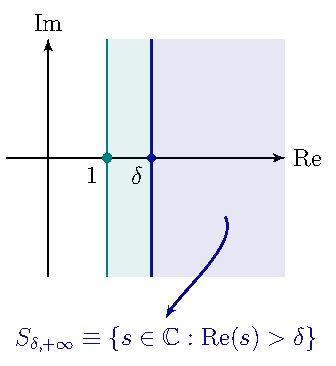
\includegraphics{Figuras/S delta infinito.pdf}
    \end{figure}
    %
    Seja $\delta>1$ e $S_{\delta, +\infty}$  
    o semi-plano dado por
    %
    \[
    S_{\delta, +\infty} 
    \equiv 
    \left\{ s\in\C :\ \Re(s) > \delta \right\}.
    \]
    %
    Para cada $n\in\N$ seja  
    $f_n: S_{\delta, +\infty}\to\C$
    a função holomorfa definida por
    %
    \[
    f_n(s) = \frac{1}{n^s} = \exp(-s\ln n).
    \]
    %
    Note que segue diretamente das definições 
    de $f_n$, $S_{\delta, +\infty}$ e de supremo que
    %
    \[
    \sup_{s\in S_{\delta,+\infty}} |f_n(s)| 
    = 
    \sup_{s\in S_{\delta,+\infty}}
    \exp(-\Re(s)\ln n) 
    \leq 
    \exp(-\delta\ln n).
    \]
    %
    Desta estimativa segue que 
    %
    \[
    \sum_{n=1}^{\infty} 
    \sup_{s\in S_{\delta,+\infty}}|f_n(s)|
    \leq 
    \sum_{n=1}^{\infty} \exp(-\delta\ln n)
    = 
    \sum_{n=1}^{\infty} \frac{1}{n^\delta}
    \]
    %
    e como $\delta > 1$, podemos garantir que 
    a série do lado direito da igualdade acima é convergente.
    Já que cada $f_n$ é holomorfa em $S_{\delta, +\infty}$, segue
    diretamente do Teste-M de Weierstrass que $\zeta$ define de fato uma holomorfa em
    $S_{\delta,+\infty}$. 
    Por fim,
    como $\delta > 1$ foi tomado arbitrariamente, segue que
    $\zeta$ é holomorfa em todo semi-plano $\Re(s) > 1$.
    
    Agora, vamos mostrar que $\zeta$ admite uma extensão meromorfa a $\C$, com apenas
    um polo simples em $s=1$ com resíduo 1. Como veremos, o argumento da extensão de
    $\zeta$ é bem mais delicado que o da extensão da função $\Gamma$. De fato,
    para realizarmos a extensão vamos precisar considerar, além da função $\Gamma$, 
    outra função especial:
    a função teta de Jacobi $\vartheta: \R\to\C$
    dada por
    %
    \begin{equation}
    \index{Função! Teta de Jacobi}
    \label{def-funcao-teta-jacobi}
        \vartheta(t) = \sum_{n=-\infty}^{\infty} e^{-\pi n^2t}.
    \end{equation}
    %
    Assim como $\Gamma$, a função $\vartheta$ também satisfaz uma equação funcional,
    a saber
    %
    \begin{equation}
    \label{eq-funcional-teta}
        \vartheta(t) = t^{-1/2}\vartheta\left( \frac{1}{t} \right), \, \forall t\neq 0.
    \end{equation}
    %
    Também vamos precisar das seguintes estimativas:
    %
    \begin{itemize}
        \item $\vartheta(t) \leq Ct^{-1/2}$, $0 < t \leq 1$;
        \item $|\vartheta(t) - 1| \leq \widetilde{C}e^{-\pi t}$, $t\geq 1$.
    \end{itemize}
    %
    Por comodidade, reunimos estes resultados nos dois lemas a seguir.
    %
    \begin{lema}
    \label{lema-eq-funcional}
        A função $\vartheta$ satisfaz a equação funcional
        %
        \[
        \vartheta(t) = t^{-1/2}\vartheta\left( \frac{1}{t} \right), \, \forall t\neq 0.
        \]
        %
    \end{lema}
    %
    \begin{proof}
        Para mostrar a validade da equação, vamos utilizar a transformada
        de Fourier de $f(x) = e^{-\pi x^2}$ e a Fórmula da Soma de Poisson 
        (Teorema \ref{teo-form-soma-poisson}). Como vimos em
        \eqref{eq-trans-fourier-gaussiana},
        %
        \[
        \widehat{f}(\xi) = \int_{-\infty}^{\infty} e^{-\pi x^2}e^{-2\pi ix\xi} \, d\xi 
                         = e^{-\pi \xi^2}.
        \]
        %
        Portanto, para cada $t>0$ fixado, podemos 
        obter a transformada de Fourier de $g(x) = e^{-\pi tx^2}$, 
        como segue
        %
        \begin{align*}
            \widehat{g}(\xi) &= 
            \int_{-\infty}^{\infty} e^{-\pi tx^2}e^{-2\pi ix\xi} \, dx 
            \\[0.3cm]
             &= \int_{-\infty}^{\infty} 
             e^{-\pi u^2}e^{-2\pi i\frac{u}{\sqrt{t}}\xi} \frac{1}{\sqrt{t}} \, du \\[0.3cm]
             &= \frac{1}{\sqrt{t}}
             \int_{-\infty}^{\infty} e^{-\pi u^2}e^{-2\pi iu\frac{\xi}{\sqrt{t}}} \, du \\[0.3cm]
             &= \frac{1}{\sqrt{t}}\exp\left( -\pi \frac{\xi^2}{t} \right),
        \end{align*}
        %
        onde na segunda igualdade acima usamos a mudança de variáveis
        $u = \sqrt{t}x$. 
        Agora, aplicando a Fórmula da Soma de Poisson obtemos
        %
        \begin{align*}
            \vartheta(t) = \sum_{n\in\Z} e^{-\pi tn^2}
                         = \sum_{n\in\Z} g(n) 
                         = \sum_{n\in\Z} \widehat{g}(n) 
                         = \frac{1}{\sqrt{t}}\sum_{n\in\Z} e^{-\pi n^2/t}
                         = \frac{1}{\sqrt{t}}\vartheta\left( \frac{1}{t} \right).
        \end{align*}
        %
    \end{proof}
    %
    \begin{lema}
    \label{lema-estimativas}
        A função $\vartheta$ satisfaz as estimativas
        %
        \begin{itemize}
            \item $\vartheta(t) \leq Ct^{-1/2}$, $0 < t \leq 1$;
            \item $|\vartheta(t) - 1| \leq \widetilde{C}e^{-\pi t}$, $t\geq 1$.
        \end{itemize}
        %
    \end{lema}
    %
    \begin{proof}
        Começamos com a primeira estimativa. Pela equação funcional \eqref{eq-funcional-teta},
        temos
        %
        \begin{align*}
            |\vartheta(t)| &= \frac{1}{\sqrt{t}}\left| \vartheta\left( \frac{1}{t} \right) \right| \\
                           &= \frac{1}{\sqrt{t}}\left| \sum_{n\in\Z} e^{-\pi n^2/t} \right| \\
                           &= \frac{1}{\sqrt{t}}\left| 1 + 2\sum_{n=1}^{\infty} e^{-\pi n^2/t} \right| \\
                           &\leq \frac{1}{\sqrt{t}}\left( 1 + 2\sum_{n=1}^{\infty} e^{-\pi n^2} \right) \\
                           &= Ct^{-1/2},
        \end{align*}
        %
        onde usamos que $e^{-\pi n^2/t} \leq e^{-\pi n^2}$ para $0 < t \leq 1$ e tomamos
        $C \equiv 1 + 2\sum_{n=1}^{\infty} e^{-\pi n^2}$.
        
        Para o segundo item, basta observar que
        %
        \begin{align*}
            |\vartheta(t) - 1| &= \left| \sum_{n\in\Z} e^{-\pi n^2t} - 1 \right| \\
                               &= \left| 1 + 2\sum_{n=1}^{\infty} e^{-\pi n^2t} - 1 \right| \\
                               &= 2\sum_{n=1}^{\infty} e^{-\pi n^2t} \\
                               &\leq 2\sum_{n=1}^{\infty} e^{-\pi nt} \\
                               &= 2\cdot\frac{e^{-\pi t}}{1 - e^{-\pi t}} \\
                               &\leq \left( \frac{2}{1 - e^{-\pi}} \right)e^{-\pi t} \\
                               &= \widetilde{C}e^{-\pi t}.
        \end{align*}
        %
    \end{proof}
    %
    Tendo estabelecido esses lemas, podemos começar a analisar as relações entre as funções
    $\Gamma$, $\zeta$ e $\vartheta$. 
    Um dos resultados mais importantes envolvendo a relação entre estas
    três funções é o Teorema \ref{teo-zeta-gamma-teta} abaixo. Antes de
    apresentar a prova deste teorema vamos precisar um lema auxiliar. 
    
    \begin{lema}
    \label{lema-aux-teo-zeta-gamma-teta}
    Para todo $s\in \C$ tal que $\Re(s)>1$, vale a identidade mostrada abaixo. 
    Além do mais, as séries e integrais que aparecem nesta expressão são todas convergentes.
    \begin{equation}
        \label{eq-aux1-lema-int-sum-teta}
        \sum_{n=1}^{\infty}\int_0^{\infty} e^{-\pi n^2u}u^{s/2 - 1} \, du
        =
        \int_0^{\infty}\sum_{n=1}^{\infty} e^{-\pi n^2u}u^{s/2 - 1} \, du
    \end{equation}
    \end{lema}
    \begin{proof}
        Vamos começar mostrando que a série que aparece no lado 
        esquerdo de \eqref{eq-aux1-lema-int-sum-teta} é absolutamente convergente para todo $s\in \C$ tal que $\Re(s)>1$. 
        
        Para provar esta convergência é necessário 
        obter uma expressão mais simples que 
        permita entender o comportamento assintótico da $n$-ésima parcela 
        desta soma quando $n\to\infty$. 
        Isto pode ser feito usando o Teorema da Mudança de Variáveis,
        fazendo $\pi n^2 u = t$, e a definição da função Gama
        como segue:
        %
        \begin{align}
        \label{eq-aux2-lema-int-sum-teta}
            \int_0^{\infty} e^{-\pi n^2u}u^{s/2 - 1} \, du 
            &= \int_0^{\infty} e^{-t}t^{s/2 - 1} \left( \frac{1}{\pi n^2} \right)^{s/2} \, dt 
            \nonumber\\[0.3cm]
            &= \pi^{-s/2}\frac{1}{n^s}\int_0^{\infty} e^{-t}t^{s/2 - 1} \, dt 
            \nonumber\\[0.3cm]
            &= \pi^{-s/2}\Gamma\left( \frac{s}{2} \right)\frac{1}{n^s}.
        \end{align}
        %
        Já que o lado direito da expressão acima é absolutamente somável, 
        quando $\Re(s)>1$, podemos concluir que a série que 
        aparece no lado esquerdo 
        de \eqref{eq-aux1-lema-int-sum-teta} é convergente.
        
        
        Sobre o lado direito da igualdade \eqref{eq-aux1-lema-int-sum-teta},
        primeiro observamos que a série que aparece nesta expressão,
        isto é, 
        \[
        \sum_{n=1}^{\infty} e^{-\pi n^2u}
        \]
        é convergente para todo $u>0$, 
        por uma aplicação direta do teste da raiz $n$-ésima. 
        Note que esta série não converge para $u=0$.
        
        Além do mais, segue do teste M de Weierstrass que para cada $s$ fixado a aplicação 
        \[
        u\longmapsto \sum_{n=1}^{\infty} e^{-\pi n^2u} u^{s/2-1}  
        \]
        é holomorfa no semiplano $\{u\in \C: \Re(u)>\delta\}$ para 
        todo $\delta>0$. Consequentemente, como $\delta>0$ é arbitrário segue que a aplicação acima define uma função complexa contínua em $(0,+\infty)$ e portanto Riemann integrável em cada um dos intervalos limitados e fechados desta semi-reta.
        
        O próximo passo na prova do lema é mostrar que para cada $s\in \C$ com $\Re(s)>1$ fixado,
        temos
        \[
        \lim_{N\to\infty}
        \int_0^{\infty}\sum_{n=N}^{\infty} e^{-\pi n^2u}u^{s/2 - 1} \, du
        =
        0.
        \]
        
        Para isto é suficiente mostrar que 
        \[
        \lim_{N\to\infty}
        \int_0^{\infty}\sum_{n=N}^{\infty} |e^{-\pi n^2u}u^{s/2 - 1}| \, du
        =
        0.
        \]
        Note que usando as mesmas cotas da prova do Teste da Integral (veja \eqref{eq-aux1-teste-integral}) temos para todo $u>0$ e $N>1$ a seguinte desigualdade:
        \begin{align}
        \label{eq-aux1-lema-int-soma-theta}
            \sum_{n=N}^{\infty} 
            |e^{-\pi n^2u}u^{s/2 - 1}|
            &=
            u^{\Re(s)/2 - 1} 
            \sum_{n=N}^{\infty} e^{-\pi n^2u}
            \nonumber\\[0.3cm]
            &\leqslant
            u^{\Re(s)/2 - 1}\
            \int_{N}^{\infty} 
            e^{-\pi u x^2}\, dx.
        \end{align}
        
        Usando coordenadas polares e o Teorema de Fubini (como no cálculo clássico da integral Gaussiana) podemos estimar a integral que aparece no lado direito da desigualdade acima. De fato, 
        \begin{align}
        \label{eq-aux2-lema-int-soma-theta}
        \left(
        \int_{N}^{\infty} e^{-\pi u x^2}\, dx
        \right)^2
        &=
        \int_{N}^{\infty}\int_{N}^{\infty}
        e^{-\pi u (x^2+y^2)}\, dx\,dy
        \nonumber\\[0.3cm]
        &=
        \iint_{[N,\infty)\times [N,\infty)}
        e^{-\pi u (x^2+y^2)}\, dx\,dy
        \nonumber\\[0.3cm]
        &\leqslant 
        \int_{0}^{\frac{\pi}{2}}
        \int_{N}^{\infty}
        e^{-\pi u r^2}\, r\,dr\,d\theta
        \nonumber\\[0.3cm]
        &=
        \frac{\pi}{2}\cdot\frac{1}{2\pi u} 
        e^{-\pi u N}
        \leqslant
        \frac{1}{u}e^{-\pi u N}.
        \end{align}
    %
    \begin{figure}[H]\centering
        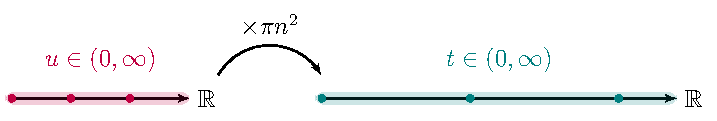
\includegraphics{Figuras/mudança de variável.pdf}
    \end{figure}
    %    
    Tomando a raiz quadrada nos dois lados da desigualdade acima e, em seguida, substituindo a cota obtida em \eqref{eq-aux1-lema-int-soma-theta} 
    ficamos com 
    \begin{align}
    \label{eq-aux3-lema-int-soma-theta}
    \sum_{n=N}^{\infty} 
    |e^{-\pi n^2u}u^{s/2 - 1}|
    \leqslant
    u^{\Re(s)/2 - 1}
    \, u^{-1/2}\, 
    e^{-\frac{\pi u N}{2}}
    =
    u^{\frac{1}{2}(\Re(s)-3)}
    e^{-\frac{\pi u N}{2}}.
    \end{align}

    Portanto, temos 
    \begin{align}
    \int_0^{\infty}\!\sum_{n=N}^{\infty} |e^{-\pi n^2u}u^{s/2 - 1}| \, du
    &\leqslant
    \int_0^{\infty}
    u^{\frac{1}{2}(\Re(s)-3)}
    e^{-\frac{\pi u N}{2}}
    \, du.
    \end{align}
    Usando a mudança de variáveis $t=\pi u N/2$ na integral que aparece no lado direito da desigualdade acima e também que $\Re(s)>1$, obtemos
    \begin{align*}
    \int_0^{\infty}\!\sum_{n=N}^{\infty} |e^{-\pi n^2u}u^{s/2 - 1}| \, du
    &\leqslant
    \frac{2}{\pi N}
    \left(\frac{2}{\pi N}\right)^{\frac{1}{2}(\Re(s)-3)}
    \int_0^{\infty}
    t^{\frac{1}{2}(\Re(s)-3)}
    e^{-t}
    \, dt
    \\[0.3cm]
    &=
    \left(\frac{2}{\pi N}\right)^{\frac{1}{2}(\Re(s)-1)}
    \int_0^{\infty}
    t^{\frac{1}{2}(\Re(s)-1)-1}
    e^{-t}
    \, dt
    \\[0.3cm]
    &=
    \left(\frac{2}{\pi N}\right)^{\frac{1}{2}(\Re(s)-1)}
    \Gamma\left(\frac{1}{2}\left(\Re(s)-1\right)\right).
    \end{align*}
    Como $\Re(s) > 1$, a desigualdade acima permite concluir que 
    \begin{align}
    \label{eq-aux4-lema-int-soma-theta}
    \lim_{N\to\infty}
    \int_0^{\infty}\sum_{n=N}^{\infty} e^{-\pi n^2u}u^{s/2 - 1} \, du
    =
    0.
    \end{align}
    
    Para finalizar, observe que temos das propriedades elementares
    de séries convergentes e da integral de Riemann 
    a seguinte igualdade
    \begin{align*}
    \int_0^{\infty}\sum_{n=1}^{\infty} e^{-\pi n^2u}u^{s/2 - 1} \, du  
    &=
    \int_0^{\infty}
    \left[ 
    \sum_{n=1}^{N-1} e^{-\pi n^2u}u^{s/2 - 1}
    +
    \sum_{n=N}^{\infty} e^{-\pi n^2u}u^{s/2 - 1} 
    \right]
    du
    \\[0.3cm]
    &=
    \sum_{n=1}^{N-1}
    \int_0^{\infty}
    e^{-\pi n^2u}u^{s/2 - 1}\, du
    +
    \int_{0}^{\infty}
    \sum_{n=N}^{\infty} e^{-\pi n^2u}u^{s/2 - 1}\, du.
    \end{align*}
    Tomando o limite quando $N\to\infty$ 
    em ambos lados da igualdade acima e 
    usando \eqref{eq-aux4-lema-int-soma-theta} finalizamos a prova do lema.
    \end{proof}
    %
    \begin{teorema}
    \label{teo-zeta-gamma-teta}
        Para todo $s\in\C$ com $\Re(s) > 1$, vale
        %
        \[
        \pi^{-s/2}\Gamma\left( \frac{s}{2} \right)\zeta(s) 
        = \frac{1}{2}\int_0^{\infty} u^{s/2 - 1}[\vartheta(u) - 1] \, du.
        \]
        %
    \end{teorema}
    %
    \begin{proof}
    A parte mais complicada da prova deste teorema já foi discutida no lema anterior e assim vamos precisar apenas juntar as peças.    
    
    De acordo com \eqref{eq-aux2-lema-int-sum-teta} 
    sabemos que para todo $\Re(s)>1$, 
    vale a seguinte igualdade %
        \[
            \int_0^{\infty} e^{-\pi n^2u}u^{s/2 - 1} \, du
            = \pi^{-s/2}\Gamma\left( \frac{s}{2} \right)\frac{1}{n^s}.
        \]
        %
        Somando, sobre $n\in\N$, ambos lados da identidade acima temos
        %
        \[
            \sum_{n\in\N} \int_0^{\infty} e^{-\pi n^2u}u^{s/2 - 1} \, du
            = 
            \displaystyle\pi^{-s/2}\Gamma\left( \frac{s}{2} \right)\sum_{n\in\N}\frac{1}{n^s} 
        \]
        Como estamos assumindo que $\Re(s)>1$ 
        podemos aplicar o Lema \ref{lema-aux-teo-zeta-gamma-teta}
        para permutar a ordem das soma e da integral
        que aparecem na igualdade acima, ficando com 
        \[
            \int_0^{\infty}
            \sum_{n\in\N} 
            e^{-\pi n^2u}u^{s/2 - 1} \, du
            = 
            \displaystyle\pi^{-s/2}\Gamma\left( \frac{s}{2} \right)\sum_{n\in\N}\frac{1}{n^s} 
        \]
Usando a definição da função $\vartheta$, segue da igualdade acima que 
%
        \[
        \int_0^{\infty} \frac{1}{2}[\vartheta(u) - 1] u^{s/2 - 1} \, du
        = 
        \displaystyle
        \pi^{-s/2}\Gamma\left( \frac{s}{2} \right)\zeta(s)
        \]
o que encerra a prova do teorema.
    \end{proof}
    
    \bigskip 
    
    
    %
    Esse último teorema merece alguns comentários. 
    Observe, primeiramente, que o lado esquerdo
    da identidade contém: 
    \begin{itemize}
        \item uma função inteira, $\pi^{s/2}$;
        
    \item uma função meromorfa em $\C$ com
    polos simples nos inteiros pares não positivos, $\Gamma(s/2)$;
    
    \item e uma função holomorfa em $\Re(s) > 1$.
    
    \end{itemize}
    
    Portanto a aplicação que leva 
    $s\longmapsto \xi(s)$ dada por
    %
    \begin{align}
    \label{def-fun-xi}
    \xi(s) = \pi^{-s/2}\Gamma\left( \frac{s}{2} \right)\zeta(s),
    \end{align}
    %
    define uma função holomorfa no semi-plano $\Re(s) > 1$.
    %
    \begin{teorema}
    \label{teo-form-reflexao-xi}
        A função $\xi$ definida em \eqref{def-fun-xi}
        admite uma continuação analítica à todo domínio $\C\setminus\{0,1\}$,
        que abuso de notação será também denotada por, 
        \[\xi:\C\setminus\{0,1\}\to\C.\]
        As suas singularidades em $s=0$ e $s=1$
        são polos simples e seus resíduos são dados por $\mathrm{res}(\xi,0)=-1$ e $\mathrm{res}(\xi,1)=1$.
        Ademais, ela satisfaz
        a seguinte equação funcional
        %
        \[
        \xi(s) = \xi(1-s), \, \forall s\in\C\setminus\{0,1\}.
        \]
        %
    \end{teorema}
    %
    \begin{proof}
        Por comodidade, consideramos a função auxiliar $\psi:\R_+\to\C$ dada por
        %
        \[
        \psi(u) = \frac{1}{2}[\vartheta(u) - 1].
        \]
        %
        A partir da equação funcional de $\vartheta$, deduzimos a seguinte equação funcional
        para $\psi$:
        %
        \begin{align*}
            \psi(u) &= \frac{1}{2}\left[\frac{1}{\sqrt{u}}\vartheta\left( \frac{1}{u} \right) - 1\right] \\
                    &= \frac{1}{2}\left[\frac{1}{\sqrt{u}}
                    \left( \vartheta\left( \frac{1}{u} \right) - 1 + 1 \right) - 1\right] \\
                    &= \frac{1}{2}\left[\frac{1}{\sqrt{u}}
                    \left( 2\psi\left( \frac{1}{u} \right) + 1 \right) - 1\right] \\
                    &= \frac{1}{\sqrt{u}}\psi\left( \frac{1}{u} \right) + \frac{1}{2\sqrt{u}} - \frac{1}{2}.
        \end{align*}
        %
        Agora, do Teorema \ref{teo-zeta-gamma-teta}, sabemos que
        %
        \begin{align*}
            \pi^{-s/2}\Gamma\left( \frac{s}{2} \right)\zeta(s) 
            = \int_0^{\infty} u^{s/2 - 1}\frac{1}{2}[\vartheta(u) - 1] \, du
            = \int_0^{\infty} u^{s/2 - 1}\psi(u) \, du.
        \end{align*}
        %
        Para calcular esta última integral, vamos dividi-la em duas parcelas e controlar
        cada uma delas:
        %
        \begin{align}
        \label{eq-aux1-teo-eq-func-zeta-completa}
        \int_0^{\infty} u^{s/2 - 1}\psi(u) \, du
        = \int_0^1 u^{s/2 - 1}\psi(u) \, du + \int_1^{\infty} u^{s/2 - 1}\psi(u) \, du.
        \end{align}
        
        %
        Para avaliar a primeira parcela do lado direito, usamos a equação funcional de $\psi$, o Teorema Fundamental do Cálculo e por último uma mudança de variáveis como segue:
        %
        \begin{align*}
            \int_0^1 u^{s/2 - 1}\psi(u) \, du 
            &= 
            \int_0^1 u^{s/2 - 1}
            \left[
                \frac{1}{\sqrt{u}}\psi\left(\frac{1}{u}\right) 
                + \frac{1}{2\sqrt{u}} - \frac{1}{2}
            \right] \, du 
            \\[0.3cm]
            &= 
            \int_0^1
            \left[
                u^{s/2 - 1}u^{-1/2}\psi\left(\frac{1}{u}\right) 
                + \frac{u^{s/2 - 3/2}}{2} - \frac{u^{s/2 - 1}}{2}
            \right] \, du
            \\[0.3cm]
            &= 
            \frac{u^{s/2 - 1/2}}{s-1}\Bigg|_0^1 - \frac{u^{s/2}}{s}\Bigg|_0^1 
            + \int_0^1 u^{s/2 - 1}u^{-1/2}\psi\left(\frac{1}{u}\right) \, du 
            \\[0.3cm]
            &= \frac{1}{s-1} - \frac{1}{s} + \int_0^1 u^{s/2 - 3/2}\psi\left(\frac{1}{u}\right) \, du 
            \\[0.3cm]
            &= \frac{1}{s-1} - \frac{1}{s} + \int_1^{\infty} v^{-s/2 - 1/2}\psi(v) \, dv.
        \end{align*}
        %
        Agora usamos esta expressão em 
        \eqref{eq-aux1-teo-eq-func-zeta-completa} e somamos as duas integrais de forma a obter a seguinte igualdade
        %
        \begin{align*}
            \int_0^{\infty} u^{s/2 - 1}\psi(u) \, du
            = \frac{1}{s-1} - \frac{1}{s} + 
            \int_1^{\infty} \left[u^{-s/2 - 1/2} + u^{s/2 - 1}\right]\psi(u) \, du.
        \end{align*}
        %
        Agora, vamos mostrar que a integral no lado direito define uma função holomorfa da variável complexa $s$.
        Para tanto, defina
        %
        \[
        g_n(s) = \int_1^n \left[ u^{s/2 - 1} + u^{-s/2 - 1/2} \right] \psi(u) \, du.
        \]
        %
        Já que o integrando acima define uma função contínua em $\C\times [1,n]$ podemos usar o Teorema de Fubini para integrar $g_n$ ao longo de  
        qualquer curva de Jordan suave por partes  
        $\y$ contida no plano complexo e desta forma concluir que
        %
        \begin{align*}
            \int_{\y} g_n(s) \, ds 
            &=\int_{\y} \left( 
            \int_1^n \left[ u^{s/2 - 1} + u^{-s/2 - 1/2} \right] \psi(u) \, du \right) \, ds 
            \\[0.3cm]
            &= \int_1^n \psi(u) \int_{\y} \left[ u^{s/2 - 1} + u^{-s/2 - 1/2} \right] \, ds \, du 
            \\[0.3cm]
            &= 0.
        \end{align*}
        %
        Vamos considerar agora a restrição de $g_n$ à faixa
        %
        \[
        S_{-M, M} = \{ s\in\C : -M \leq \Re(s)\leq M \}
        \]
        %
        e mostrar que estas restrições 
        convergem uniformemente para $
        g:S_{-M, M}\to\C$ dada por
        %
        \[
        g(s) 
        = 
        \int_1^{\infty} 
        \left[ 
        u^{s/2 - 1} + u^{-s/2 - 1/2} 
        \right] 
        \psi(u) \, du.
        \]
        
        
        %
        Já sabemos que $g$ está bem definida em $\Re(s) > 1$. Usando o Lema \ref{lema-conv-abs-cond-int-imp}
        sabemos que para mostrar que $g$ está bem
        definida em toda a faixa $S_{-M, M}$, basta mostrar que
        %
        \[
        \int_1^{\infty} \left| u^{s/2 - 1} + u^{-s/2 - 1/2} \right|\cdot|\psi(u)| \, du < +\infty,
        \qquad \forall s\in S_{-M, M}.
        \]
        %
        De fato, para $u\geq 1$ temos que
        %
        \[
        |u^{s/2 - 1} + u^{-s/2 - 1/2}| \leq 2u^{|\Re(s)|/2 - 1/2} \leq 2u^{M/2 - 1/2} \leq 2u^K,
        \]
        %
        sendo $K = M/2 - 1/2$. 
        Do Lema \ref{lema-estimativas}
        e da definição de $\psi$ temos a seguinte 
        equivalência para algumas constantes positivas
        $C_1$ e $C_2$
        %
        \[
        |\vartheta(u) - 1| 
        \leq 
        C_1\, e^{-\pi u} 
        \qquad\iff\qquad 
        |\psi(u)| 
        \leq 
        C_2\, e^{-\pi u},
        \qquad \forall u\geqslant 1.
        \]
        %
        Usando estas três últimas desigualdades e uma comparação básica entre exponenciais e polinômios 
        concluímos que
        %
        \begin{align*}
        \int_1^{\infty} 
        \left| u^{s/2 - 1} + u^{-s/2 - 1/2} \right|\cdot|\psi(u)| 
        \, du
        &\leqslant
        \int_1^{\infty} 2u^{K}\cdot C_2\, e^{\pi u} \, du
        \\
        &\leq 
        \int_1^{\infty} \left( 2u^K\ C_2\ 
        e^{-\pi u/2} \right)e^{-\pi u/2}\, du 
        \\
        &\leq 
        C_3\int_1^{\infty} e^{-\pi u/2} \, du \\
        &< +\infty.
        \end{align*}
        %
        Usando estimativas idênticas às acima, 
        podemos verificar que 
        %
        \begin{align*}
            \sup_{s\in S_{-M,M}} |g_n(s) - g(s)| 
            &\leq 
            \sup_{s\in S_{-M,M}}
            \int_n^{\infty} \left| u^{s/2 - 1} + u^{-s/2 - 1/2} \right|\cdot|\psi(u)| \, du 
            \\[0.3cm]
            &\leq 
            K_1\int_n^{\infty} e^{-\pi u/2} \, du 
            \\
            &= 
            K_2\, e^{-\pi n/2} 
            \xrightarrow{\ n\to\infty\ } 0.
        \end{align*}
        %
        Como para cada $n\in\N$ a função $g_n$ é analítica e que $g_n$ converge uniformemente para $g$,
        quando $n\to\infty$, na faixa $S_{-M, M}$, segue que
        $g$ é analítica em $S_{-M, M}$. 
        
        Por fim, como o parâmetro $M$ que determina a largura da faixa $S_{-M,M}$ é arbitrário, segue que a aplicação
        %
        \begin{equation}
        \label{eq-aux1-cont-analitica-xi}
        s 
        \longmapsto 
        \int_1^{\infty} \left[ u^{s/2 - 1} + u^{-s/2 - 1/2} \right] \psi(u) \, du
        \end{equation}
        %
        define uma função inteira.
        
        Considere então a extensão meromorfa de $\xi$ dada pelo lado direito da igualdade
        %
        \[
        \xi(s) = \frac{1}{s-1} - \frac{1}{s} + \int_1^{\infty} [u^{s/2 - 1} + u^{-s/2 - 1/2}]\psi(u) \, du.
        \]
        %
        Notando que a soma das duas primeiras parcelas e o integrando na igualdade acima são invariantes pela aplicação $s\longmapsto 1-s$ podemos verificar  imediatamente que $\xi(s) = \xi(1-s)$. De fato, 
        %
        \begin{align*}
            \xi(1-s) &= \frac{1}{1-s-1} - \frac{1}{1-s} 
            + \int_1^{\infty} [u^{1/2 - s/2 - 1} + u^{-1/2 + s/2 - 1/2}]\psi(u) \, du \\
            &= \frac{1}{s-1} - \frac{1}{s} + \int_1^{\infty} [u^{s/2 - 1} + u^{-s/2 - 1/2}]\psi(u) \, du \\
            &= \xi(s).
        \end{align*}
        %
    \end{proof}
    %
    Com esse teorema, podemos olhar agora para a função $\zeta$.
    %
    \begin{teorema}
    \label{teo-cont-zeta}
        A função $\zeta:\{ s\in\C : \Re(s) > 1 \} \to \C$ admite uma continuação meromorfa a todo $\C$,
        com apenas um polo simples em $s=1$ com resíduo $1$.
    \end{teorema}
    %
    \begin{proof}
        Já sabemos que para todo $s\in\C$ tal que $\Re(s) > 1$ vale
        %
        \[
        \xi(s) = \pi^{-s/2}\Gamma\left(\frac{s}{2}\right)\zeta(s).
        \]
        %
        Também sabemos que, nessa região, $\Gamma(s/2)\neq 0$. Portanto, é lícito escrever
        %
        \[
        \zeta(s) 
        = 
        \pi^{s/2}\frac{1}{\Gamma(s/2)}\xi(s), 
        \qquad \forall s\in\C, \, \Re(s) > 1.
        \]
        %
        Como $1/\Gamma$ é uma função inteira com zeros 
        de multiplicidade 1 nos inteiros pares não positivos,
        podemos afirmar 
        que existe uma função 
        $g:\C\to\C$ holomorfa com $g(0)\neq 0$ tal que
        %
        \[
        \frac{1}{\Gamma(s)} = s\, g(s) 
        \qquad\implies\qquad
        \frac{1}{\Gamma(s/2)} = \frac{s}{2}\cdot g\Big(\frac{s}{2}\Big).
        \]
        %
        Portanto,
        %
        \begin{align*}
            \zeta(s) &= 
            \pi^{s/2}\frac{1}{\Gamma(s/2)}\xi(s)
            \\[0.3cm]
            &=
            \pi^{s/2}\ \frac{s}{2}\ g\Big(\frac{s}{2}\Big)
            \left( \frac{1}{s-1} - \frac{1}{s} + h(s) \right) 
            \\[0.3cm]
            &= \frac{\pi^{s/2}}{2}\left( \frac{s}{s-1} - 1 + s\, h(s) \right)g\Big(\frac{s}{2}\Big),
        \end{align*}
        %
        sendo $h$ a função inteira que aparece em \eqref{eq-aux1-cont-analitica-xi} 
        ao longo 
        da prova do teorema anterior. 
        O lado direito da identidade acima
        é a extensão procurada, 
        haja vista que define uma função holomorfa em $\C\setminus\{1\}$.
        Resta, portanto, mostrar que $s=1$ é 
        polo simples e calcular seu resíduo. Para tanto,
        basta calcular
        %
        \begin{align*}
            \lim_{s\to 1} (s-1)\zeta(s) 
            &= \lim_{s\to 1} \frac{\pi^{s/2}}{2}\Big( s - (s-1) + (s-1)\,s\,h(s) \Big)g\Big(\frac{s}{2}\Big)\\[0.3cm]
            &= \frac{\pi^{1/2}}{2}\lim_{s\to 1} \left[ s\, g\Big(\frac{s}{2}\Big)\right] \\[0.3cm]
            &= \frac{\pi^{1/2}}{2}\lim_{s\to 1} \frac{2}{\Gamma(s/2)} \\[0.3cm]
            &= \frac{\pi^{1/2}}{2}\cdot\frac{2}{\Gamma(1/2)} \\[0.3cm]
            &= \frac{\pi^{1/2}}{2}\cdot\frac{2}{\pi^{1/2}} \\[0.3cm]
            &= 1.
        \end{align*}
        %
    \end{proof}
    %
    A seguir, vamos mostrar uma representação da função $\zeta$
    em termos de um produtório.
    %
    \begin{teorema}[A Fórmula de Produto de Euler]
    \label{teo-form-prod-euler}
    \index{Fórmula!do Produto de Euler}
        Para todo $s\in\C$ tal que $\Re(s) > 1$, temos
        %
        \[
        \prod_{p\in\mathbb{P}} 
        \left(1 - \frac{1}{p^s} \right)
        \zeta(s) 
        =
        1,
        \]
        %
        onde o produtório que aparece acima converge uniformemente nas
        partes compactas do semi-plano $\{Re(s)>1\}$ e é realizado sobre o conjunto de todos os números primos. Consequentemente, 
        se $\Re(s)>1$ temos $\zeta(s)\neq 0$ e 
        também vale a famosa fórmula de produto de Euler 
        \[
        \zeta(s) 
        =
        \prod_{p\in\mathbb{P}} 
        \left(1 - \frac{1}{p^s} \right)^{-1}.
        \]
    \end{teorema}
    %
    \begin{proof}
        Nesta prova, é de importância fundamental o fato de que a
        série de Dirichlet da função zeta de Riemann, ou seja,
        %
        \[
        \sum_{n=1}^{\infty} \frac{1}{n^s}
        \]
        %
        converge {\bf absolutamente} no semi-plano $\Re(s) > 1$.
        
        Para provar o teorema primeiro vamos mostrar, por indução em $n$, uma identidade auxiliar, que envolve certos produtos parciais. Em seguida, argumentamos que é possível 
        tomar o limite destes produtos parciais, quando $n$ tende a infinito e obter a fórmula desejada. 
        
        O primeiro passo da indução, mencionada acima, consiste em observar que para todo $s\in\C$ tal que $\Re(s)>1$ temos
        da propriedades elementares de séries absolutamente convergentes que
        %
        \begin{align}
        \label{eq:tirando-pares-form-prod}
            \frac{1}{2^s}\zeta(s) 
            &= \frac{1}{2^s}\left(
            1 + \frac{1}{2^s} + \frac{1}{2^s} 
            + \frac{1}{3^s} + \frac{1}{4^s}
            + \frac{1}{5^s} + \cdots
            \right)
            \nonumber\\
            &= \frac{1}{2^s} + \frac{1}{4^s} + \frac{1}{6^s}
            + \frac{1}{8^s} + \frac{1}{10^s} + \cdots.
        \end{align}
        %
        Daí, subtraindo \eqref{eq:tirando-pares-form-prod} da expressão
        em série de Dirichlet de $\zeta$, ficamos com
        %
        \begin{equation}
        \label{eq:zeta-sem-pares}
            \left( 1 - \frac{1}{2^s} \right)\zeta(s) 
            = 1 + \frac{1}{3^s} + \frac{1}{5^s} 
            + \frac{1}{7^s} + \frac{1}{9^s} + \cdots.
        \end{equation}
        %
        Antes de prosseguir com o argumento, é importante frisar um
        ponto: a priori, se $A$ é um conjunto infinito enumerável qualquer e $(a_n)_{n\in A}$ é uma coleção arbitrária de números complexos, indexada em $A$, então a soma dos $a_n$'s sobre $A$, isto é,
        %
        \[
        \sum_{n\in A} a_n,
        \]
        %
        pode não estar bem definida. 
        Isto ocorre, por exemplo, quando a família das 
        somas sobre os subconjuntos finitos de $A$, 
        forma um conjunto de números complexos 
        com mais de um ponto de acumulação. 
        Em outras palavras, dependendo da ordem em que realizamos a
        soma podemos construir somas parciais que convergem para 
        distintos limites ou mesmo que nem sequer convergem.
        Este fenômeno é comum quando lidamos, por exemplo, 
        com séries condicionalmente convergentes.
        
    
        Por outro lado, quando lidamos com uma família de números complexos absolutamente somável, então a ordem
        em que realizamos a soma não é relevante e, 
        nesse caso, o símbolo acima está bem definido.
        
        
        Feita esta ressalva, observamos que todas as somas (finitas e infinitas) que aparecem nos argumentos abaixo 
        são somas absolutamente convergentes. 
        O que permite usar, sem ambiguidade, a notação acima.
        
        Antes de voltar ao argumento de indução vamos introduzir mais algumas notações. Dado um número primo $p$ denotamos o conjunto 
        dos múltiplos de $p$ por 
        %
        \[
        p\N \equiv  \{ p, 2p, 3p, \dots \}.
        \]
        %
        E usaremos a notação 
        %
        \[
        \N(2, 3, \dots, p_n) 
        = \{ 2, 3, 4, \dots \} 
        \setminus \bigcup_{p\in\{2, 3, \dots, p_n\}} p\N,
        \]
        %
        onde $p_n$ o $n$-ésimo primo, para denotar o 
        conjunto de todos os números naturais maiores ou iguais a dois
        que não são múltiplos de $2,3,5,7,11,\ldots p_n$. 
        
        Utilizando esta notação observe que podemos reescrever \eqref{eq:zeta-sem-pares} como 
        %
        \[
        \sum_{n\in\N(2)} \frac{1}{n^s}.
        \]
        %
        Procedendo analogamente, temos que
        %
        \[
        \frac{1}{3^s}\left( 1 - \frac{1}{2^s} \right)\zeta(s)
        = \frac{1}{3^s} + \frac{1}{9^s} + \frac{1}{15^s} + \cdots
        \]
        %
        e, portanto,
        %
        \[
        \left(1 - \frac{1}{3^s}\right)\left(1 - \frac{1}{2^s}\right)\zeta(s)
        = 1 + \frac{1}{5^s} + \frac{1}{7^s} + \frac{1}{11^s} + \cdots
        = 1 + \sum_{n\in\N(2,3)} \frac{1}{n^s}.
        \]
        %
        Segue então por indução em $n$ que
        %
        \begin{align*}
            \left(1 - \frac{1}{p_n^s}\right)
            \cdots
            \left(1 - \frac{1}{3^s}\right)
            \left(1 - \frac{1}{2^s}\right)\zeta(s)
            &= 1 + \sum_{n\in\N(2,3, \dots, p_n)} \frac{1}{n^s} 
            \\[0.5cm]
            \big\Downarrow
            \\[0.5cm]
            \left|
            \prod_{j=1}^n \left(1 - \frac{1}{p_j^s}\right)\zeta(s) - 1
            \right|
            = \left|
            \sum_{j\in\N(2,3, \dots, p_n)} \frac{1}{j^s}
            \right|
            &\leq \sum_{j=p_n}^{\infty} \left|\frac{1}{j^s}\right|,
            \,\quad \forall n\geq 1.
        \end{align*}
        %
        Como a cauda da série de Dirichlet 
        de $\zeta$ converge para $0$,
        segue que
        %
        \[
        \left[
        \lim_{n\to\infty} \prod_{j=1}^n \left(1 - \frac{1}{p_j^s}\right)
        \right]\zeta(s)
        = 1
        \qquad \iff \qquad
        \prod_{p\in\mathbb{P}} \left(1 - \frac{1}{p^s}\right)\zeta(s)
        = 1.
        \]
        %
        
        Como consequência da igualdade acima podemos afirmar que $\zeta(s)\neq 0$ no semi-plano
        $\Re(s) > 1$. 
        
        
        Por fim, lembrando que se uma sequência
        de números complexos $(b_n)_{n\in\N}$ 
        é tal que $b_n\to b\neq 0$,
        então temos que $1/b_n \to 1/b$. 
        Desta propriedade elementar de sequências convergentes e da identidade acima podemos concluir finalmente que 
        %
        \[
        \zeta(s) 
        = \prod_{p\in\mathbb{P}} \left(1 - \frac{1}{p^s}\right)^{-1}.
        \]
        %
    \end{proof}
    %
    
    \subsection{Regiões Livres de Zeros da Função Zeta de Riemann}
    
    Agora, vamos analisar as regiões nas quais a função zeta não se anula.
    O último teorema nos garante que no semi-plano $\Re(s)>1$, $\zeta(s) \neq 0$.
    Da equação funcional para $\zeta$, sabemos que os inteiros pares não positivos,
    $\{0, -2, -4, -6, \dots\}$ são todos zeros dessa função, geralmente chamados
    \textbf{zeros triviais} de $\zeta$.
    %
    \begin{figure}[H]\centering
        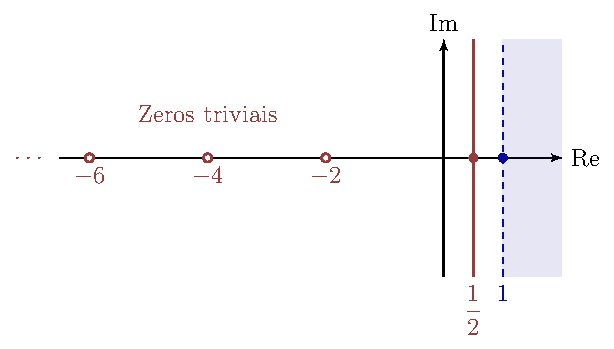
\includegraphics{Figuras/zeros triviais.pdf}
    \end{figure}
    %
    Usando a simetria de $\zeta$ em torno da reta $\Re(s) = 1/2$, vamos argumentar que,
    a menos dos zeros triviais, $\zeta(s)\neq 0$ para todo $s\in\C$ com $\Re(s)<0$.
    
    De fato, como
    %
    \[
    \xi(s) = \pi^{-s/2}\Gamma\left(\frac{s}{2}\right)\zeta(s)
    \]
    %
    para todo $s\in\C$ com $\Re(s)>1$, temos que $\xi$ não se anula nesse semi-plano,
    pois nenhum dos fatores se anula. Daí, segue da equação funcional
    %
    \[
    \xi(s) = \xi(1-s)
    \]
    %
    que $\xi$ também não se anula no semi-plano $\Re(s) < 0$, ou seja, que $\xi(1-s)\neq 0$
    para todo $s\in\C$ com $\Re(s)>1$. Ora, mas
    %
    \[
    \xi(1-s) = \pi^{-(1-s)/2}\Gamma\left(\frac{1-s}{2}\right)\zeta(1-s).
    \]
    %
    Note que $\pi^{-(1-s)/2}\neq 0$ e $\Gamma((1-s)/2)\neq 0$. Portanto, devemos
    necessariamente ter $\zeta(1-s)\neq 0$, ou seja, $\zeta$ não se anula no
    semi-plano $\Re(s) < 0$.
    %
    \begin{figure}[H]\centering
        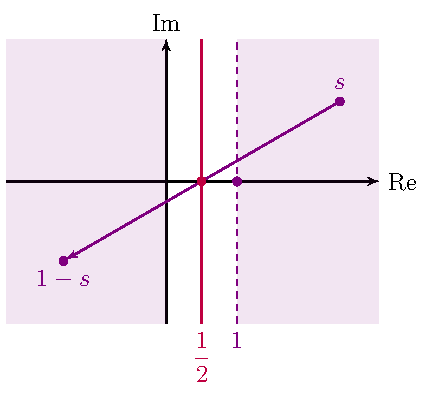
\includegraphics{Figuras/espelho de s.pdf}
    \end{figure}
    %
    \begin{center}
        \red{Falar das quádruplas de zeros}
        
        \red{Falar de $\overline{\zeta(\overline{s})}$}
    \end{center}
    %
    
    
    \subsubsection*{Algumas propriedades adicionais da função Gama}
    %
    Vamos tratar de mais algumas propriedades da função $\Gamma$ que nos
    serão úteis mais à frente, a saber: a ordem de crescimento de $1/\Gamma$
    e sua expressão em termos de uma fórmula de produto.
    %
    \begin{teorema}
    \label{teo-ordem-cresc-inv-gama}
        A função $1/\Gamma$ é tal que
        %
        \[
        \left| \frac{1}{\Gamma(s)} \right| \leq C_1e^{C_2|s|\ln|s|} \, \forall s\in \C
        \]
        %
        para um par de constantes $C_1,C_2\in\R$,
        ou seja, a ordem de crescimento de $1/\Gamma$ é 1 no sentido de que
        para todo $\e>0$ existe $C(\e)>0$ tal que
        %
        \[
        \left| \frac{1}{\Gamma(s)} \right| \leq C(\e)e^{C_2|s|^{1+\e}} \, \forall s\in C.
        \]
        %
    \end{teorema}
    %
    \begin{proof}
        Nesta demonstração, vamos precisar usar dois fatos importantes obtidos previamente,
        a saber, a equação funcional de $\Gamma$:
        %
        \[
        \Gamma(s)\Gamma(1-s) = \frac{\pi}{\sen(\pi s)}, \, \forall s\in\C\setminus\Z
        \]
        %
        e a extensão de $\Gamma$:
        %
        \[
        \Gamma(s) = \sum_{n=0}^{\infty} \frac{(-1)^n}{n!(n+s)} 
                    + \int_0^{\infty} e^{-t}t^{s-1} \, dt, \, 
                    \forall s\in\C\setminus\{0, -1, -2, \dots\}.
        \]
        %
        Com essas duas identidades, podemos escrever
        %
        \begin{align}
        \label{eq-expressao-inv-gama}
            \frac{1}{\Gamma(s)} &= \Gamma(1-s)\frac{\sen(\pi s)}{\pi} \nonumber \\ 
                                &= \left( \sum_{n=0}^{\infty} \frac{(-1)^n}{n!(n+1-s)} \right)
                                \frac{\sen(\pi s)}{\pi}
                                + \left( \int_0^{\infty} e^{-t}t^{-s} \, dt \right)
                                \frac{\sen(\pi s)}{\pi}, \, \forall s\in\C\setminus\Z.
        \end{align}
        %
        Com isso, dividiremos a prova em duas etapas. Primeiro, vamos estimar a parcela integral
        da identidade acima e, após isso, vamos estimar a parcela em série.
        
        Para a primeira etapa, começamos mostrando que
        %
        \begin{equation}
        \label{eq-cota-int-parte-real}
            \int_1^{\infty} e^{-t} t^{\sigma - 1} \, dt \leq e^{(\sigma + 1)\ln(\sigma + 1)},
        \end{equation}
        %
        sendo $\Re(s) = \sigma \geq 0$. De fato, escolha $n\in\N$ tal que 
        $\sigma \leq n\leq \sigma+1$. Então, usando o fato de que $0< 1/t \leq 1$ e também
        a monotonicidade do logaritmo e da exponencial, temos
        %
        \begin{align*}
            \int_1^{\infty} e^{-t}t^{\sigma - 1} \, dt 
            &\leq \int_1^{\infty} e^{-t}t^{\sigma} \, dt \\
            &\leq \int_1^{\infty} e^{-t} t^n \, dt \\
            &= \Gamma(n+1) \\
            &= n! \\
            &\leq n^n \\
            &= e^{n\ln n} \\
            &\leq e^{(\sigma + 1)\ln(\sigma + 1)}.
        \end{align*}
        %
        Essa desigualdade nos permite concluir que
        %
        \[
        \left| \int_1^{\infty} e^{-t} t^s \, dt \right| \leq e^{(|\sigma|+1)\ln(|\sigma|+1)}, \, 
        \forall s\in\C.
        \]
        %
        Para majorar a segunda parcela de \eqref{eq-expressao-inv-gama}, vamos majorar
        $e^{(|\sigma|+1)\ln(|\sigma|+1)}$. Essa majoração será dividida em duas partes.
        
        Para $0 < |s| < 1$, podemos escrever
        %
        \begin{align*}
            e^{(|\sigma|+1)\ln(|\sigma|+1)} &\leq e^{(|s|+1)\ln(|s|+1)} \\
                                            &= e^{|s|\ln(|s|+1)}e^{\ln(|s|+1)} \\
                                            &\leq 2\exp\left[ |s|\ln\left( |s|(1 + 1/|s|) \right) \right] \\
                                            &\leq 2e^{|s|\ln|s|}e^{|s|\ln(1 + 1/|s|)}.
        \end{align*}
        %
        Observe que, pela Regra de L'Hôpital,
        %
        \begin{align*}
            \lim_{s\to 0} \left[ |s|\ln\left( 1 + \frac{1}{|s|} \right) \right]
            &= \lim_{s\to 0} \frac{\ln(1 + 1/|s|)}{1/|s|} \\
            &= \lim_{x\to 0^+} \frac{\ln(1 + 1/x)}{1/x} \\
            &= \lim_{x\to 0^+} (1 + 1/x)^{-1}(-1/x^2)/(-1/x^2) \\
            &= 0.
        \end{align*}
        %
        Portanto, dado $\e=1$ existe $0<\delta<1$ tal que se $|s|<\delta$ então
        %
        \[
        \left| \frac{\ln(1 + 1/|s|)}{1/|s|} \right| < 1 \implies |\ln(1 + 1/|s|)| \leq 2/|s| 
                                                        \implies |s|\ln(1+1/|s|) \leq 2.
        \]
        %
        Voltando à estimativa, temos que para $0<|s|<1$ vale que
        %
        \begin{align*}
            e^{(|\sigma|+1)\ln(|\sigma|+1)} &\leq 2e^2e^{|s|\ln|s|}.
        \end{align*}
        %
        Agora, para $1\leq|s|$, temos
        %
        \begin{align*}
            e^{(|\sigma|+1)\ln(|\sigma|+1)} &\leq e^{(|s|+1)\ln(|s|+1)} \\
                                            &\leq e^{2|s|\ln(2|s|)} \\
                                            &= e^{2|s|(\ln|s| + \ln 2)} \\
                                            &\leq e^{2|s|\ln|s|}e^{2|s|}.
        \end{align*}
        %
        %
        \begin{center}
            \red{aqui eu não consegui uma cota uniforme em $s$...}
        \end{center}
        %
        Ademais, sabemos que $|\sen(\pi s)| \leq e^{\pi |s|}$ pela Fórmula de Euler. Portanto,
        a segunda parcela de \eqref{eq-expressao-inv-gama} é majorada por
        %
        \begin{equation}
            \left| \left( \int_0^{\infty} e^{-t}t^{-s} \, dt \right)\frac{\sen(\pi s)}{\pi} \right|
            \leq
            C_1(s)e^{C_2|s|\ln|s|},
        \end{equation}
        %
        sendo
        %
        \[
        \begin{cases}
            C_1(s) = \frac{2}{\pi}e^{\pi + 2}, \, 0 < |s| < 1 \\
            C_1(s) = \frac{1}{\pi}e^{(\pi + 2)|s|}, \, 1\leq |s|
        \end{cases} \qquad \text{ e } \qquad
        \begin{cases}
            C_2 = 1, \, 0 < |s| < 1 \\
            C_2 = 2, \, 1\leq |s|
        \end{cases}.
        \]
        %
        
        Agora, precisamos majorar a parcela que envolve a série em \eqref{eq-expressao-inv-gama}.
        Para tanto, vamos dividir nossa análise em dois casos: $|\Im(s)| > 1$ e $|\Im(s)|\leq 1$.
        
        Se $|\Im(s)| > 1$, então $|n+1-s| \geq 1$, como ilustra o diagrama abaixo.
        %
        \begin{figure}[H]\centering
            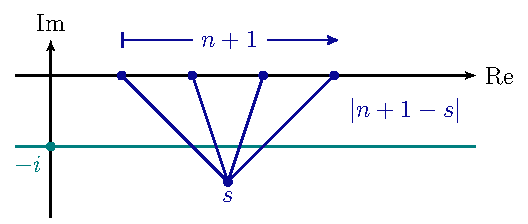
\includegraphics{Figuras/Im(s)>1.pdf}
        \end{figure}
        %
        Daí, segue pela desigualdade triangular que
        %
        \[
        \left| \sum_{n=0}^{\infty} \frac{(-1)^n}{n!(n+1-s)} \right| 
        \leq \sum_{n=0}^{\infty} \frac{1}{n!|n+1-s|} 
        \leq \sum_{n=0}^{\infty} \frac{1}{n!}
        = e.
        \]
        %
        Portanto, como $|\sen(\pi s)| \leq e^{\pi |s|}$ temos que para todo $s\in\C$ com $|\Im(s)|>1$
        vale
        %
        \[
        \left| \left(\sum_{n=0}^{\infty} \frac{(-1)^n}{n!(n+1-s)}\right)\frac{\sen(\pi s)}{\pi} \right|
        \leq \frac{e}{\pi} e^{\pi |s|}
        \red{\leq C_4e^{C_5|s|\ln|s|}},
        \]
        %
        sendo $C_4 = $ e $C_5 = $ ...
        
        Agora, se $|\Im(s)| \leq 1$, escolhemos $k\in\Z$ tal que
        %
        \[
        k - \frac{1}{2} \leq \Re(s) < k + \frac{1}{2}.
        \]
        %
        Isso reduz nossa análise a retângulos, como o ilustrado abaixo.
        %
        \begin{figure}[H]\centering
            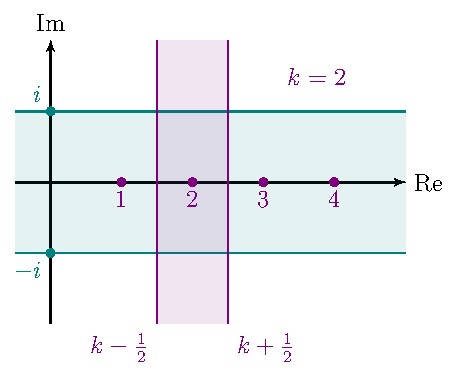
\includegraphics{Figuras/K>=1.pdf}
        \end{figure}
        %
        Para terminar, dividimos a análise novamente em dois sub-casos: $k\geq 1$ e $k\leq 0$.
        
        \paragraph{Caso i): $k\geq 1$.} Nesse caso, podemos escrever
        %
        \begin{align*}
            \left(\sum_{n=0}^{\infty} \frac{(-1)^n}{n!(n+1-s)}\right)\frac{\sen(\pi s)}{\pi}
            = \frac{(-1)^{k-1}\sen(\pi s)}{(k-1)!(k-s)\pi} +
            \left(\sum_{\substack{n\in\N \\ n\neq k}}^{\infty} 
            \frac{(-1)^n}{n!(n+1-s)}\right)\frac{\sen(\pi s)}{\pi}.
        \end{align*}
        %
        Temos que
        %
        \[
        \left|\lim_{s\to k} \frac{\sen(\pi s)}{(k-s)\pi}\right| 
        = \left|\lim_{s\to k} \frac{\pi\cos(\pi s)}{-\pi}\right|
        = 1.
        \]
        %
        Ademais, se $n\neq k$ então $|n+1-s| \geq 1/2$ e, portanto,
        %
        \begin{align*}
            \left|\left(\sum_{\substack{n\in\N \\ n\neq k}}^{\infty} 
            \frac{(-1)^n}{n!(n+1-s)}\right)\frac{\sen(\pi s)}{\pi}\right|
            \leq 2\sum_{\substack{n\in\N \\ n\neq k}} \frac{1}{n!}e^{\pi |s|}
            \leq C_3e^{\pi |s|},
        \end{align*}
        %
        sendo $C_3 = 2e$.
        %
        \paragraph{Caso ii): $k\leq 0$.} Nesse caso, temos $\Re(s) < 1/2$ já que estamos
        supondo que 
        %
        \[
        k - \frac{1}{2} \leq \Re(s) < k + \frac{1}{2}.
        \]
        %
        Portanto,
        %
        \[
        |n+1-s| \geq |n+1 - i\Im(s) - \Re(s)| \geq |n+1 - \Re(s)| \geq \frac{1}{2},
        \]
        %
        conforme ilustra o diagrama abaixo. 
        %
        \begin{figure}[H]\centering
            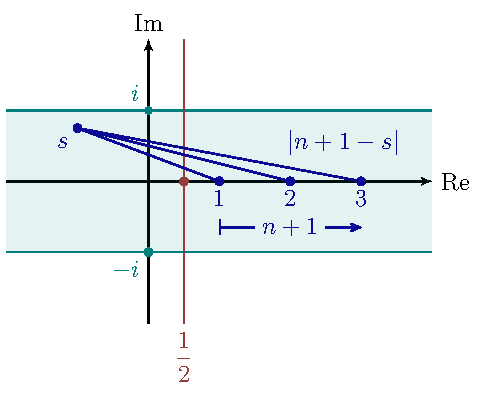
\includegraphics{Figuras/K<=0.pdf}
        \end{figure}
        %
        Logo, temos a estimativa
        %
        \[
        \left|\left(\sum_{n=0}^{\infty} \frac{(-1)^n}{n!(n+1-s)}\right)\frac{\sen(\pi s)}{\pi}\right|
        \leq C_3e^{\pi |s|},
        \]
        %
        sendo $C_3 = 2e$ novamente.
        
        Juntando todas as estimativas obtidas, obtemos finalmente
        %
        \begin{align*}
            \left| \frac{1}{\Gamma(s)} \right| 
            &\leq \left|\left(\sum_{n=0}^{\infty} \frac{(-1)^n}{n!(n+1-s)}\right)\frac{\sen(\pi s)}{\pi}\right|
            + \left| \left( \int_1^{\infty} e^{-t} t^{-s} \, dt \right)\frac{\sen(\pi s)}{\pi} \right| \\[0.3cm]
            &\leq C_3e^{\pi |s|} + C_1(s)e^{C_1|s|\ln|s|} \\[0.3cm]
            &\leq 4C_3(e^{-1/e})e^{\pi |s|} + C_1(s)e^{C_1|s|\ln|s|} \\[0.3cm]
            &\leq 4C_3e^{|s|\ln|s|} + C_1(s)e^{C_1|s|\ln|s|} \\[0.3cm]
            &\leq K_1(s)e^{K_2|s|\ln|s|},
        \end{align*}
        %
        onde a constante $e^{-1/e}$ aparece por ser o valor mínimo da função $e^{x\ln x}, x>0$. De fato,
        derivando essa expressão e igualando a derivada a zero, temos
        %
        \[
        (e^{x\ln x})' = e^{x\ln x}(1 + \ln x) = 0 \iff x = 1/e.
        \]
        %
        Derivando novamente, temos que
        %
        \[
        (e^{x\ln x})'' = e^{x\ln x}(1 + \ln x)^2 + e^{x\ln x}\frac{1}{x}
        \]
        %
        e, em $x = 1/e$, a segunda derivada vale $e^{1 - 1/e} > 0$, de modo que $x = -1/e$
        é, de fato, ponto de mínimo.
    \end{proof}
    %
    
    \medskip
    
    Agora, vamos demonstrar uma belíssima fórmula de produto para $1/\Gamma$.
    %
    \begin{teorema}
    \label{teo-form-prod-inv-gama}
        Para todo $s\in\C$ temos
        %
        \[
        \frac{1}{\Gamma(s)} = e^{\y s}s\prod_{n=1}^{\infty} \left( 1 + \frac{s}{n} \right)e^{-s/n},
        \]
        %
        sendo
        %
        \[
        \y \equiv \lim_{N\to\infty} \sum_{j=1}^N \frac{1}{j} - \ln N
        \]
        %
        a constante de Euler-Mascheroni.
        \index{Constante de Euler-Mascheroni}
    \end{teorema}
    %
    \begin{proof}
        A demonstração é uma aplicação quase direta do Teorema de Hadamard, uma vez que provamos
        no teorema anterior que $1/\Gamma$ tem ordem de crescimento $1$.
        
        Antes, entretanto, vamos mostrar a existência do limite que define $\y$. Para tanto,
        observe que
        %
        \begin{align*}
            \sum_{j=1}^N \frac{1}{j} - \ln N 
            = \sum_{j=1}^N \frac{1}{j} - \int_1^N \frac{1}{x} \, dx
            = \frac{1}{N} + \sum_{j=1}^{N-1} \int_j^{j+1} \left(\frac{1}{j} - \frac{1}{x}\right) \, dx.
        \end{align*}
        %
        Pelo Teorema do Valor Médio aplicado à função $f(y) = 1/y$, sabemos que
        %
        \[
        \left| \frac{1}{j} - \frac{1}{x} \right| \leq \frac{1}{j^2}, \, \forall n\leq x\leq n+1.
        \]
        %
        Portanto,
        %
        \[
        \sum_{j=1}^N \frac{1}{j} - \ln N = \frac{1}{N} + \sum_{j=1}^{N-1} a_j,
        \]
        %
        sendo
        %
        \[
        |a_j| = \left| \int_j^{j+1} \left(\frac{1}{j} - \frac{1}{x}\right) \, dx \right| \leq \frac{1}{j^2}.
        \]
        %
        Logo, sabemos que
        %
        \[
        \sum_{j=1}^{\infty} a_j \leq \sum_{j=1}^{\infty} \frac{1}{j^2} = \frac{\pi^2}{6},
        \]
        %
        de modo que existe
        %
        \[
        \lim_{N\to\infty} \sum_{j=1}^N \frac{1}{j} - \ln N = \sum_{j=1}^{\infty} a_j.
        \]
        %
        
        Feito isto, basta aplicarmos o Teorema de Hadamard a $1/\Gamma$ para obter constantes
        $A,B\in\C$ tais que
        %
        \[
        \frac{1}{\Gamma(s)} = e^{As + B}s\prod_{n=1}^{\infty} \left(1 + \frac{s}{n}\right)e^{-s/n}, \,
        \forall s\in\C.
        \]
        %
        Podemos reescrever essa identidade como
        %
        \[
        1 = e^{As + B}s\Gamma(s)\prod_{n=1}^{\infty} \left(1 + \frac{s}{n}\right)e^{-s/n}.
        \]
        %
        Tomando o limite quando $s\to 0$ e lembrando que $\lim_{s\to 0}s\Gamma(s) = 1$, segue que
        %
        \[
        e^B = 1 \iff B = 0.
        \]
        %
        Por outro lado, tomando $s=1$ na identidade temos
        %
        \begin{align*}
            1 = \frac{1}{\Gamma(1)} &= e^A \prod_{n=1}^{\infty} \left(1 + \frac{1}{n}\right)e^{-1/n} \\
                                &= e^A \lim_{N\to\infty}\prod_{n=1}^{N} \left(1 + \frac{1}{n}\right)e^{-1/n} \\
                                &= e^A \lim_{N\to\infty}\prod_{n=1}^{N} \exp(\ln(1+1/n) - 1/n) \\
                                &= e^A \lim_{N\to\infty} \exp\left[ -\sum_{n=1}^N \frac{1}{n} +
                                                \sum_{n=1}^N \ln(1 + 1/n) \right] \\
                                &= e^A \lim_{N\to\infty} \exp\left[ -\sum_{n=1}^N \frac{1}{n} +
                                                \ln\left( \prod_{n=1}^N (1 + 1/n) \right) \right] \\
                                &= e^A \lim_{N\to\infty} \exp\left[ -\sum_{n=1}^N \frac{1}{n} +
                                                \ln\left( \prod_{n=1}^N \frac{n+1}{n} \right) \right] \\
                                &= e^A \lim_{N\to\infty} \exp\left[ -\sum_{n=1}^N \frac{1}{n} +
                                                \ln(N+1) \right] \\
                                &= e^Ae^{-\y},
        \end{align*}
        %
        donde segue que $A = \y + 2\pi ik, k\in\Z$. Ora, mas como $\Gamma(s)\in\R, \, \forall s\in\R$,
        segue que $k = 0$ e $A = \y$, completando a demonstração.
    \end{proof}
    %
    
    \medskip
    
    Agora, vamos voltar a tratar da função $\zeta$. Mostramos
    anteriormente que essa função não se anula fora da faixa
    $0 \leq \Re(s) \leq 1$. Vamos, agora, mostrar que
    $\zeta$ não se anula na reta $\Re(s) = 1$ (isso implicará,
    pela simetria da função, que ela não se anula na reta 
    $\Re(s) = 0$ e, portanto, que todos os zeros não triviais
    da $\zeta$ estão no interior da faixa $0<\Re(s)<1$.
    
    Para provar o resultado, vamos precisar de três lemas
    auxiliares.
    %
    \begin{lema}
    \label{lema-log-zeta}
        Para todo $s\in\C$ tal que $\Re(s)>1$, vale a identidade
        %
        \[
        \log\zeta(s) = \sum_{p,m} \frac{p^{-ms}}{m} 
                     = \sum_{n=1}^{\infty} c_nn^{-s},
        \]
        %
        onde $p$ percorre o conjunto dos números primos, 
        $m$ percorre o conjunto dos números naturais,
        $c_n\geq 0$ para todo $n$ e a convergência das séries
        é absoluta.
    \end{lema}
    %
    \begin{proof}
        Frisamos, novamente, que a notação $\log\zeta(s)$ \textbf{não} denota uma composta
        entre o ramo principal do logaritmo e a função $\zeta$, mas sim uma nova função, que
        é chamada de logaritmo da $\zeta$ no sentido do Lema \ref{lema-ramo-log}. 
        Para demonstrar o resultado, vamos primeiramente assumir que $s\in\R$ e $s>1$ e provar
        a identidade para esse caso. Em seguida, usaremos extensão analítica para verificar que a
        identidade vale em todo o semi-plano $\Re(s)>1$.
        
        Então, supondo $s>1$, podemos representar o logaritmo natural através da seguinte série 
        de potências
        %
        \[
        \ln\left( \frac{1}{1-x} \right) = \sum_{m=1}^{\infty} \frac{x^m}{m},
        \]
        %
        que é válida para $0\leq x < 1$ e converge absolutamente nesse intervalo. 
        Daí, recordando que $\zeta(s)\in\R_+$ para $s\in\R$
        e usando a representação em produto para $\zeta$, segue que
        %
        \[
        \ln(\zeta(s)) = \ln\left( \prod_{p\in\mathbb{P}} \frac{1}{1 - p^{-s}} \right)
                      = \sum_{p\in\mathbb{P}} \ln\left( \frac{1}{1 - p^{-s}} \right)
                      = \sum_{p,m} \frac{p^{-ms}}{m}.
        \]
        %
        Agora, tomando $c_n = 1/m$ se $n = p^m$ e $c_n = 0$ caso contrário, podemos reescrever
        %
        \[
        \ln(\zeta(s)) = \sum_{n=1}^{\infty} c_n n^{-s}.
        \]
        %
        Até o momento, mostramos que essa expressão é válida para $s\in(1, +\infty)$.
        Ora, mas o lado direito é analítico no semi-plano $\Re(s)>1$, pelo mesmo argumento que 
        usamos para mostrar que $\zeta$ admitia uma representação em série de Dirichlet nesse
        semi-plano. Além disso, sabemos que a função zeta não se anula em $\Re(s)>1$, de modo que
        existe $\log\zeta(s)$ pelo Lema \ref{lema-ramo-log}.
        
        Sabemos que esse ramo do logaritmo para $\zeta$ coincide com o somatório acima no intervalo
        $(1, +\infty)$, que contém ponto de acumulação. Portanto, pelo 
        Corolário \ref{cor-unicidade-ext-analiticas}, podemos representar $\log\zeta(s)$
        por
        %
        \[
        \log\zeta(s) = \sum_{n=1}^{\infty} c_n n^{-s},
        \]
        %
        para todo $s\in\C$ com $\Re(s)>1$.
    \end{proof}
    %
    \begin{lema}
    \label{lema-des-cosseno}
        Para todo $\theta\in\R$, vale a desigualdade
        %
        \[
        3 + 4\cos\theta + \cos 2\theta \geq 0.
        \]
        %
    \end{lema}
    %
    \begin{proof}
        Basta notar que
        %
        \[
        3 + 4\cos\theta + \cos 2\theta 
        = 3 + 4\cos\theta + 2\cos^2\theta - 1
        = 2(1 + \cos\theta)^2 \geq 0.
        \]
        %
    \end{proof}
    %
    O último lema que precisaremos para demonstrar o 
    teorema desejado é consequência dessa desigualdade.
    %
    \begin{lema}
    \label{lema-log-produto-zetas}
        Para todos $\sigma>1$ e $t\in\R$, vale a desigualdade
        %
        \[
        \ln|\zeta^3(\sigma)\zeta^4(\sigma + it)\zeta(\sigma + 2it)|
        \geq 0.
        \]
        %
    \end{lema}
    %
    \begin{proof}
        Seja $s = \sigma + it$. Note que
        %
        \[
        \Re(n^{-s})
        = \Re(e^{-(\sigma + it)\ln n})
        = \Re(e^{-\sigma\ln n}e^{-it\ln n})
        = e^{-\sigma\ln n}\cos(t\ln n)
        = n^{-\sigma}\cos(t\ln n).
        \]
        %
        Usando esse fato e o Lema \ref{lema-log-zeta}, temos
        %
        \begin{align*}
            \ln|\zeta^3(\sigma)\zeta^4(\sigma + it)\zeta(\sigma + 2it)|
            &= \ln|\zeta^3(\sigma)| + \ln|\zeta^4(\sigma + it)|
                                    + \ln|\zeta(\sigma + 2it)| \\
            &= 3\ln|\zeta(\sigma)| + 4\ln|\zeta(\sigma + it)| 
                                   + \ln|\zeta(\sigma + 2it)| \\
            &= 3\Re(\log(\zeta(\sigma))) + 4\Re(\log(\zeta(\sigma + it)))
                                         + \Re(\log(\zeta(\sigma + 2it))) \\
            &= \sum_{n=1}^{\infty} c_n \left[\Re(n^{-\sigma}) 
                                        + \Re(n^{-\sigma - it})
                                        + \Re(n^{-\sigma} - 2it) \right] \\
            &= \sum_{n=1}^{\infty} c_n n^{-\sigma}\left[3 + 4\cos\theta_n
                                                        + \cos 2\theta_n \right],
        \end{align*}
        %
        sendo $\theta_n = t\ln n$ e $c_n\geq 0$ como definidos na prova
        do Lema \ref{lema-log-zeta}. Pelo Lema \ref{lema-des-cosseno}, segue que
        %
        \[
        \sum_{n=1}^{\infty} c_n n^{-\sigma}\left[3 + 4\cos\theta_n
                                                        + \cos 2\theta_n \right]
        \geq 0,
        \]
        %
        e temos o resultado desejado.
    \end{proof}
    %
    
    \medskip
    
    
    Podemos agora enunciar precisamente e demonstrar o teorema desejado.
    %
    \begin{teorema}
    \label{teo-zeta-nao-nula-re1}
        A função $\zeta$ não se anula na reta $\Re(s) = 1$, ou seja,
        $\zeta(1 + it) \neq 0$ para todo $t\in\R$.
    \end{teorema}
    %
    \begin{proof}
        Suponha, por absurdo, que $\zeta(1 + it_0) = 0$ para algum 
        $t_0\in\R^*$. Como $\zeta$ é holomorfa em $1 + it_0$, existe
        uma vizinhança desse ponto tal que
        %
        \[
        \zeta(s) = (s - (1 + it_0))^n g(s),
        \]
        %
        onde $g(s)$ é uma função holomorfa e que não se anula em $1 + it_0$
        na vizinhança. 
        %
        \begin{center}
            {\bf DIAGRAMA DA VIZINHANÇA}
        \end{center}
        %
        Daí, para $2 > \sigma > 1$ temos
        %
        \[
        |\zeta(\sigma + it_0)|^4 = |\sigma-1|^{4n}|g(1 + it_0)|^4
                                 \leq C_1(\sigma-1)^4,
        \]
        %
        sendo $C_1 = |g(1+it_0)|^4$. Ademais, como $s=1$ é polo simples
        de $\zeta$, sabemos que
        %
        \[
        |\zeta(\sigma)|^3 = \frac{C_2}{(\sigma - 1)^3},
        \]
        %
        para alguma constante positiva $C_2$. Por último, como $\zeta$ 
        também é holomorfa em $\sigma + 2it_0$, segue que
        $|\zeta(\sigma + 2it_0)|$ é limitado na vizinhança que estamos
        considerando por, digamos, $C_3 > 0$. Portanto,
        %
        \[
        |\zeta(\sigma)^3\zeta^4(\sigma + it_0)\zeta(\sigma + 2it_0)|
        \leq C_1C_2C_3(\sigma - 1) \xrightarrow{\sigma\to 1} 0,
        \]
        %
        ou seja,
        %
        \[
        \ln|\zeta(\sigma)^3\zeta^4(\sigma + it_0)\zeta(\sigma + 2it_0)| 
        \xrightarrow{\sigma\to 1} -\infty,
        \]
        %
        contrariando o Lema \ref{lema-log-produto-zetas}. Portanto,
        $\zeta$ não se anula na reta $\Re(s) = 1$, como afirmado.
    \end{proof}
    %